\renewcommand{\algorithmicrequire}{\textbf{Input:}}
\newcommand{\deflet}{\textbf{let}}
\newcommand{\mystate}[1]{\STATE \textbf{let} {{}#1}}
\newcommand{\mystop}[1]{\STATE \textbf{stop} \myss{\myangle{{{}#1}}, s'}}
\newcommand{\mystopp}[1]{\STATE \textbf{stop} \myss{\myangle{{{}#1}}}}
\newcommand{\myss}[1]{${{}#1}$}
\newcommand{\myangle}[1]{\langle {{}#1} \rangle}
\newcommand{\myif}[1]{\IF{\myss{{{}#1}}}}
\newcommand{\myelse}[1]{\ELSIF{\myss{{{}#1}}}}


\newcommand{\State}{\STATE}
\newcommand{\If}{\IF}
\newcommand{\Else}{\ELSE}
\newcommand{\EndIf}{\ENDIF}
\newcommand{\Switch}{\SWITCH}
\newcommand{\EndSwitch}{\ENDSWITCH}
\newcommand{\Case}{\CASE}
\newcommand{\EndCase}{\ENDCASE}
\newcommand{\Return}{\RETURN}
\newcommand{\For}{\FOR}
\newcommand{\EndFor}{\ENDFOR}
\newcommand{\ElsIf}{\ELSIF}

\newcommand{\Append}[2]{\STATE \textbf{let} #2 := #2 + $^{\an{}}$ #1}
\newcommand{\LetNDST}[4]{\LetND{#1}{#2} \textbf{such that} #3 \textbf{if possible; otherwise} #4}


\newcommand{\SWITCH}[1]{\STATE \textbf{switch} #1\ \textbf{do} \begin{ALC@g}}
\newcommand{\ENDSWITCH}{\end{ALC@g}\STATE \textbf{end switch}}
\newcommand{\CASE}[1]{\STATE \textbf{case} #1\textbf{:} \begin{ALC@g}}
\newcommand{\ENDCASE}{\end{ALC@g}}
\newcommand{\CASELINE}[1]{\STATE \textbf{case} #1\textbf{:} }
\newcommand{\DEFAULT}{\STATE \textbf{default:} \begin{ALC@g}}
\newcommand{\ENDDEFAULT}{\end{ALC@g}}
\newcommand{\DEFAULTLINE}[1]{\STATE \textbf{default:} }
\newcommand{\Function}[1]{\STATE \textbf{function} \myss{{{}#1}}}
\newcommand{\EndFunction}{\STATE \textbf{end function}}

\newcommand{\Let}[2]{\STATE \textbf{let} #1 := #2 }
\newcommand{\LetND}[2]{\STATE \textbf{let} #1 $\leftarrow$ #2 }

\setcounter{section}{0}
\renewcommand{\thesection}{\Alph{section}}

\appendix

\onecolumn

\section{The Concepts of Web Model}

%所有和SPRESSO的不同点放在同一个章节中一起说明。

Our formal security analysis of UPPRESSO is based on 
the general Dolev-Yao web model in SPRESSO~\cite{SPRESSO}. 
This web model is designed independently of a specific web application and closely mimics published (de-facto) standards and specifications for the web, for instance, the HTTP/1.1 and HTML5 standards and associated (proposed) standards. 
So far, the web model has been employed to analyze both trace-based authentication and indistinguishability/privacy properties for web applications.
Therefore, we formalize UPPRESSO in the web model to prove the authentication and privacy properties for UPPRESSO.

To facilitate the definition of UPPRESSO, however, 
we have some difference from SPRESSO. 
In particular, we remove some processes and 
add some function symbols for asymmetric encryption/decryption.
In this section, we present the model of the web infrastructure, along with the following changes and additions compared to SPRESSO:
\begin{itemize}
\item For constants $C$, we add the $\mathbb{P}$ as the set of points on the chosen elliptic curve over a finite field, which has been described in section~\ref{sec:UPPRESSO}.
\item We add the function symbols $\mathsf{multiply}(\cdot, \cdot)$, $\mathsf{reverse}(\cdot)$, and $\mathsf{checkvalid}(\cdot)$, representing the Elliptic Curve calculations.
\item We remove the DNS servers and messages in UPPRESSO. In UPPRESSO, however, we only have one centralized IdP server, and 
all RPs know the relevant information of the IdP in advance.
So all DNS requests are generated spontaneously by the browser, 
not introduced by our scripts.
\end{itemize}






\begin{comment}

\subsection{Functions Symbols}

Since our model is using ECC(Elliptic Curve Cryptography) to encrypt/decrypt the data,
we add the following symbols to the signature $\Sigma$ for the terms and messages:

\begin{itemize}
  \item $\mathbb{E}$ is an elliptic curve over a finite field $\mathbb{F}_q$, $G$ is a base point(or generator) of $\mathbb{E}$ and the order of $G$ is a prime number n.
  \item $[t]P$ means using asymmetric key $t$ to encrypt the point $P=[p]G$ on the elliptic curve where $p$ is the actual plaintext.
  \item $[t^{-1}]C$ means using the reverse of $t$ to decrypt the point $C=[c]G=[tm]G$ on the elliptic curve where $c$ is the cipertext.  
  \item $\str{isValid}(P)$ checks whether $P$ is a valid point on the elliptic curve. That is to say whether $P=[m]G$ for the base point $G$ and some nonce $m$.
\end{itemize}

\subsection{DNS servers}

%如果是自己编写的脚本引入了DNS请求,那就需要在模型中考虑DNS服务器,UPPRESSO可以不需要考虑。

In SPRESSO, when receiving an e-mail address, 
RP needs to send DNS requests to DNS servers manually 
to fetch the information of the IdP server. 
Since there may be various DNS servers in SPRESSO, 
DNS server security issues need to be given special consideration.
As a result, DNS servers are added into the formal model of SPRESSO.

In UPPRESSO, however, we only have one centralized IdP server, and 
all RPs know the relevant information of the IdP in advance.
So all DNS requests are generated spontaneously by the browser, 
not introduced by our scripts.
Therefore, we remove DNS servers from the formal model of UPPRESSO.

\end{comment}


\subsection{Communication Model}
We follow the SPRESSO to describe the basic concepts of the DY-style communication model.

\subsubsection{Terms, Messages and Events}

The signature $\Sigma$ for the terms and
messages in this work can be described as the following sets of symbols:
\begin{itemize}
\item constants $C = \addresses\,\cup\, \mathbb{S}\cup\mathbb{P}\cup  \{\True,\bot,\notdef\}$ where the four sets are pairwise disjoint,
$\addresses$ is interpreted to be a set of (IP) addresses,
and $\mathbb{S}$ is interpreted to be the set of ASCII strings
  (including the empty string $\varepsilon$),
and $\mathbb{P}$ is interpreted to be the set of points on the chosen elliptic curve over a finite field where $G \in \mathbb{P}$ is the base point (or generator),
\item function symbols for public keys, (a)symmetric
  en\-cryp\-tion/de\-cryp\-tion, signatures, elliptic curve multiplication, reversing elliptic curve multiplication scalar, and checking point is valid on the chosen elliptic curve: $\mathsf{pub}(\cdot)$,
  $\enc{\cdot}{\cdot}$, $\dec{\cdot}{\cdot}$, $\encs{\cdot}{\cdot}$,
  $\decs{\cdot}{\cdot}$, $\sig{\cdot}{\cdot}$,
  $\checksig{\cdot}{\cdot}$,  $\unsig{\cdot}$,
  $\mathsf{multiply}(\cdot, \cdot)$,$\mathsf{reverse}(\cdot)$,
  and $\mathsf{checkvalid}(\cdot)$,
\item $n$-ary sequences $\an{}, \an{\cdot}, \an{\cdot,\cdot},
  \an{\cdot,\cdot,\cdot},$ etc., and
\item projection symbols $\pi_i(\cdot)$ for all $i \in \mathbb{N}$.
\end{itemize}

The equational theory associated with $\Sigma$ is shown as follows:
\begin{align*}
\dec{\enc x{\pub(y)}}{y} &= x\\
\decs{\encs x{y}}{y} &= x\\
\mathsf{multiply}(x, \mathsf{multiply}(y, P)) &= \mathsf{multiply}(y, \mathsf{multiply}(x, P))\\
\mathsf{multiply}(\mathsf{reverse}(x), \mathsf{multiply}(x, P)) &= P \text{\;\;if\ } P \in \mathbb{P}\\
\checksigThree{\sig{x}{y}}{x}{\pub(y)} &= \True\\
\mathsf{checkvalid}(\mathsf{multiply}(x, P)) &= \True  \text{\;\;if\ } P \in \mathbb{P}\\
\mathsf{checkvalid}(P) &= \bot  \text{\;\;if\ } P \not\in \mathbb{P}\\
\pi_i(\an{x_1,\dots,x_n}) &= x_i \text{\;\;if\ } 1 \leq i \leq n \\
\proj{j}{\an{x_1,\dots,x_n}} &= \notdef \text{\;\;if\ } j
\not\in \{1,\dots,n\}
\end{align*}

\begin{definition}[Terms]\label{def:terms}
  We denote the set of variables $X$ and an infinite set of nonces $\nonces$. For $N\subseteq\nonces$, the set of \textbf{terms} over $\Sigma\cup N\cup X$, $\gterms_N(X)$ can be defined as usual: 
  (1) If $t\in N\cup X$, then $t \in \gterms_N(X)$ is a term. 
  (2) If $f \in \Sigma$ is an $n$-ary function symbol in $\Sigma$ for some $n\ge 0$ and  $t_1,\ldots,t_n \in \gterms_N(X)$, then $f(t_1,\ldots,t_n) \in \gterms_N(X)$ is a term.
  (3) If for some $n\ge 0$ and  $t_1,\ldots,t_n \in \gterms_N(X)$, then n-ary sequence <$t_1,\ldots,t_n$> $\in \gterms_N(X)$ is a term. 
  (4) If the n-ary sequence <$t_1,\ldots,t_n$> $\in \gterms_N(X)$, then projection symbol $\pi_i(\an{x_1,\dots,x_n}) \in \gterms_N(X)$ is a term.
\end{definition}

\begin{definition}[Messages and Protomessages]\label{def:messages}
  The set $\messages$ of messages (over $\nonces$) is defined to be
  the set of terms without variables (ground terms), i.e., $\messages :=\gterms_{\nonces}$.
  The set of protomessages, $\messages^\nu$ is defined to be the set of terms with only the predefined set of variables $V_{\text{process}} = \{\nu_1, \nu_2, \dots\}$ (called placeholders), i.e., $\messages^\nu := \gterms_N(V_{\text{process}})$.
\end{definition}

\begin{definition}[Normal Form]
  Let $t$ be a term. The \emph{normal form} of $t$ is acquired by reducing the function symbols from left to right as far as possible  using the equational theory. For a term $t$, we denote its normal form as $t\nf$.
\end{definition}

\begin{definition}[Pattern Matching]
  Let $\mi{pattern} \in \terms(\{*\})$ be a term containing the
  wildcard (variable $*$). We say that a term $t$ \emph{matches}
  $\mi{pattern}$ iff $t$ can be acquired from $\mi{pattern}$ by
  replacing each occurrence of the wildcard with an arbitrary term
  (which may be different for each instance of the wildcard). We write
  $t \sim \mi{pattern}$.

  For a term $t'$ we write $t'|\, \mi{pattern}$ to denote the term
  that is acquired from $t'$ by removing all immediate subterms of
  $t'$ that do not match $\mi{pattern}$.
\end{definition}


  For example, for a pattern $p = \an{\top,*}$ we have that $\an{\top,42} \sim p$, $\an{\bot,42} \not\sim p$, and \[\an{\an{\bot,\top},\an{\top,23},\an{\str{a},\str{b}},\an{\top,\bot}} |\, p = \an{\an{\top,23},\an{\top,\bot}}\ .\]


\begin{definition}[Variable Replacement]
  Let $N\subseteq \nonces$, $\tau \in \gterms_N(\{x_1,\ldots,x_n\})$,
  and $t_1,\ldots,t_n\in \gterms_N$. By
  $\tau[t_1\!/\!x_1,\ldots,t_n\!/\!x_n]$ we denote the term obtained
  from $\tau$ by replacing all occurrences of $x_i$ in $\tau$ by
  $t_i$, for all $i\in \{1,\ldots,n\}$.
\end{definition}


\begin{definition}[Events and Protoevents]
  An \emph{event (over $\addresses$ and $\messages$)} is a term of the
  form $\an{a, f, m}$, for $a$, $f\in \addresses$ and $m \in
  \messages$, where $a$ is interpreted to be the receiver address and
  $f$ is the sender address. We denote by $\events$ the set of all
  events. Events over $\addresses$ and $\messages^\nu$ are called
  \emph{protoevents} and are denoted $\events^\nu$. By
  $2^{\events\an{}}$ (or $2^{\events^\nu\an{}}$, respectively) we
  denote the set of all sequences of (proto)events, including the
  empty sequence (e.g., $\an{}$, $\an{\an{a, f, m}, \an{a', f', m'},
    \dots}$, etc.). 
\end{definition}

\subsubsection{Atomic Processes, Systems and Runs}

\begin{definition}[Generic Atomic Processes]
The atomic process is the modelling web nodes, in the form p=($I^p$, $Z^p$, $R^p$, $s_0^p$). The definitions of these notations is described as below.
\begin{itemize}
\item $I^p$ is the set of addresses that the process listens to, where $I^p \subseteq \addresses$.
\item  $Z^p$ is the set of \textbf{states} that describes the process. The state is the formal \textbf{term}, where $Z^p \subseteq \terms(V_{\text{process}})$. For any new state $s$ and any sequence of nonces  $(\eta_1, \eta_2, \dots)$ we demand that $s[\eta_1/\nu_1,  \eta_2/\nu_2, \dots] \in Z^p$.
\item $R^p$ is the set of \textbf{relations} $R$ between the input event $e$, state $z \in Z^p$ and an output events sequence $E$, the new state $z' \in Z^p$. It means that, at one time point, while the process is on state $s$ and receive the event $e$, it would transition to state $s'$ and send the events $E$ to other process. There is $R^p\subseteq (\events \times Z^p) \times (2^{\events^\nu\an{}}
  \times \terms(V_{\text{process}}))$. 
\item $s_0^p$ is an initial state.
\end{itemize}
\end{definition}

\begin{definition}[Systems]
A \emph{system} $\process$ is a  (possibly infinite) set of processes \aps.
\end{definition}

\begin{definition}[Configurations]
 The configuration of system represents the instantaneous state of the system at the exact moment.
  A \emph{configuration of a system $\process$} is a tuple $(S, E, N)$
  where the state of the system $S$ maps every atomic process  $p\in \process$ to its current state $S(p)\in Z^p$, the sequence of  waiting events $E$ is an infinite sequence $(e_1, e_2, \dots)$ of events waiting to be delivered, and $N$ is an infinite sequence of nonces  $(n_1, n_2, \dots)$.
\end{definition}

\begin{definition}[Concatenating sequences]
  For a term $a = \an{a_1, \dots, a_i}$ and a sequence $b = (b_1, b_2,
  \dots)$, we define the \emph{concatenation} as $a \cdot b := (a_1,
  \dots, a_i, b_1, b_2, \dots)$.
  
\end{definition}

\begin{definition}[Subtracting from Sequences]
  For a sequence $X$ and a set or sequence $Y$ we define $X \setminus
  Y$ to be the sequence $X$ where for each element in $Y$, a
  non-deterministically chosen occurence of that element in $X$ is
  removed.
\end{definition}

\begin{definition}[Processing Steps]\label{def:processing-step}
  The processing step is the system migrating from configurations ($S, E, N$) to ($S', E', N'$) by processing an event $e \in E$.
  A \emph{processing step of the system $\process$} is of the form
  \[(S,E,N) \xrightarrow[p \rightarrow E_{\text{out}}]{e_\text{in}
    \rightarrow p} (S', E', N')\]
  where
  \begin{enumerate}
  \item $(S,E,N)$ and $(S',E',N')$ are configurations of $\process$,
  \item $e_\text{in} = \an{a, f, m} \in E$ is an event,
  \item $p \in \process$ is a process,
  \item $E_{\text{out}}$ is a sequence (term) of events
  \end{enumerate}
  such that there exists 
  \begin{enumerate}
  \item a sequence (term)
    $E^\nu_{\text{out}} \subseteq 2^{\events^\nu\an{}}$ of protoevents,
  \item a term $s^\nu \in \gterms_{\nonces}(V_{\text{process}})$, 
  \item a sequence $(v_1, v_2, \dots, v_i)$ of all placeholders appearing in $E^\nu_{\text{out}}$ (ordered lexicographically),
  \item a sequence $N^\nu = (\eta_1, \eta_2, \dots, \eta_i)$ of the first $i$ elements in $N$ 
  \end{enumerate}
  with
  \begin{enumerate}
  \item $((e_{\text{in}}, S(p)), (E^\nu_{\text{out}}, s^\nu)) \in R^p$
    and $a \in I^p$,
  \item $E_{\text{out}} = E^\nu_{\text{out}}[m_1/v_1, \dots, m_i/v_i]$
  \item $S'(p) = s^\nu[m_1/v_1, \dots, m_i/v_i]$ and $S'(p') = S(p')$ for all $p' \neq p$
  \item $E' = E_{\text{out}} \cdot (E \setminus \{e_{\text{in}}\})$ 
  \item $N' = N \setminus N^\nu$ 
  \end{enumerate}
\end{definition} 

\begin{definition}[Runs]
  Let $\process$ be a system, $E^0$ be sequence of events, and $N^0$ be
  a sequence of nonces. A \emph{run $\rho$ of a system $\process$
    initiated by $E^0$ with nonces $N^0$} is a finite sequence of
  configurations $((S^0, E^0, N^0),\dots,(S^n, E^n, N^n))$ or an infinite sequence
  of configurations $((S^0, E^0, N^0),\dots)$ such that $S^0(p) = s_0^p$ for
  all $p \in \process$ and $(S^i, E^i, N^i) \xrightarrow{} (S^{i+1},
  E^{i+1}, N^{i+1})$ for all $0 \leq i < n$ (finite run) or for all $i \geq 0$  
  (infinite run).

  We denote the state $S^n(p)$ of a process $p$ at the end of a run $\rho$ by $\rho(p)$.
\end{definition}

\subsubsection{Atomic Dolev-Yao Processes}  

We next define
atomic Dolev-Yao processes, for which we require that the
messages and states that they output can be computed (more
formally, derived) from the current input event and
state. For this purpose, we first define what it means to
derive a message from given messages.




\begin{definition}[Deriving Terms]
  Let $M$ be a set of ground terms. We say that \emph{a
    term $m$ can be derived from $M$ with placeholders $V$} if there
  exist $n\ge 0$, $m_1,\ldots,m_n\in M$, and $\tau\in
  \gterms_{\emptyset}(\{x_1,\ldots,x_n\} \cup V)$ such that $m\equiv
  \tau[m_1/x_1,\ldots,m_n/x_n]$. We denote by $d_V(M)$ the set of all
  messages that can be derived from $M$ with variables $V$.
\end{definition}
For example, $a\in d_{\{\}}(\{\enc{\an{a,b,c}}{\pub(k)}, k\})$.

\begin{definition}[Atomic Dolev-Yao Process] \label{def:adyp} An \emph{atomic Dolev-Yao process
    (or simply, a DY process)} is a tuple $p = (I^p, Z^p,$ $R^p,
  s^p_0)$ such that $(I^p, Z^p, R^p, s^p_0)$ is an atomic process and
  (1) $Z^p \subseteq \gterms_{\nonces}$ (and hence, $s^p_0\in
  \gterms_{\nonces}$), and (2) for all events $e \in \events$,
  sequences of protoevents $E$, $s\in \gterms_{\nonces}$, $s'\in
  \gterms_{\nonces}(V_{\text{process}})$, with $((e, s), (E, s')) \in R^p$ it holds
  true that $E$, $s' \in d_{V_{\text{process}}}(\{e,s\})$.
\end{definition}

\begin{definition}[Atomic Attacker Process]\label{def:atomicattacker}
  An \emph{(atomic) attacker process for a set of sender addresses
    $A\subseteq \addresses$} is an atomic DY process $p = (I, Z, R,
  s_0)$ such that for all events $e$, and $s\in \gterms_{\nonces}$ we
  have that $((e, s), (E,s')) \in R$ iff $s'=\an{e, E, s}$ and
  $E=\an{\an{a_1, f_1, m_1}, \dots, \an{a_n, f_n, m_n}}$ with $n \in
  \mathbb{N}$, $a_1,\dots,a_n\in \addresses$, $f_0,\dots,f_n\in A$,
  $m_1,\dots,m_n\in d_{V_{\text{process}}}(\{e,s\})$.
\end{definition}


\subsubsection{Scripting Processes}

\begin{definition}[Scripting Processes]
 A scripting process is the modelling JavaScript code, as a relation $R$, representing the server-defined functions, while the input and output are handled by the browser. There is, $R\subseteq \terms \times
  \terms(V_{\text{script}})$ such that for all $s \in \terms$, $s' \in \terms(V_{\text{script}})$ with $(s, s') \in R$ it follows that $s'\in d_{V_{\text{script}}}(s)$.
\end{definition}

\begin{definition}[Attacker Script]
  The attacker script $\Rasp$ outputs everything that is derivable
  from the input, i.e., $\Rasp=\{(s, s')\mid s\in \terms, s'\in
  d_{V_{\text{script}}}(s)\}$.
\end{definition}


\subsection{Web Systems Model}
\label{app:websystemmodel}


The architecture of the web and its applications are represented through an model known as a web system. This system encompasses a set of DY processes, which may be infinite in number, to depict various components such as web browsers, servers, and potential adversaries capable of compromising these elements.
It also contains a set of scripting processes, including the honest and malicious processes.

\begin{definition}[Web Systems]
We can formulate the web infrastructure as a web system of form $\mathcal{WS}$=($\mathcal{W}$, $\mathcal{S}$, $\mathtt{script}$, $E^0$), where $\mathcal{W}$ is the set of atomic processes containing both honest and malicious processes, $\mathcal{S}$ is the set of scripting processes including honest and malicious scripts, $\mathtt{script}$ is the set of concrete script codes related to specific scripting processes in $\mathcal{S}$, and $E^0$ is the set of events acceptable to the processes in $\mathcal{W}$.
\end{definition}

In the following sections, we will formulate UPPRESSO system based on the web system model. Based on the UPPRESSO web system model, we will give the formal analysis of security and privacy.  


\section{The Formal Model of Basic Messages}
We now provide some more details about data and message formats that are needed for the formal treatment of the web model and the analysis of UPPRESSO presented in the rest of the appendix.

\subsection{Data Format}
\begin{definition}[Sequence]
A sequence is the term of the form $t=\an{t_1, t_2, \dots, t_n}$, where the elements in the sequence are ordered. Here we define the following notations of sequence:
\begin{itemize}
\item There is a set $s$, $t \subsetPairing s$ means that $t_1,\dots,t_n \in s$. 
\item $\left. x \inPairing t\right. \iff \exists
  i: \left. t_i = x\right.$.
\item $t \plusPairing y$ represents the sequence
  $\an{t_1,\dots,t_n,y}$.  
\item For a finite set $M = \{m_1, \dots,m_n\}$,
  $\an{M} = \an{m_1,\dots,m_n}$. 
\end{itemize}
\end{definition}

\begin{definition}[Dictionary]
A dictionary is a term of the form $d = \an{\an{k_1, v_1}, \dots, \an{k_n, v_n}}$, where the keys $k_1, \dots, k_n$ are unique. We define the following operations of dictionary:
\begin{itemize}
\item $d[k_i]=v_i$.
\item $d[k]=\an{} \text{\;\;if\ } k \not\in \an{k_1, \dots, k_n}$.
\item $d-k_i = \an{\an{k_1, v_1}, \dots, \an{k_{i-1}, v_{i-1}}, \an{k_{i+1}, v_{i+1}}, \dots, \an{k_n, v_n}}$.
\item $d+\an{k_x, v_y} = \an{\an{k_1, v_1}, \dots, \an{k_n, v_n}, \an{k_x, v_x}}$.
\end{itemize}
\end{definition}


\begin{definition}[Pointer]
A pointer $\ptr{p}$ is the sequence of non-negative integers, which points the exact element in a term. For example, there is the term $\tau=\an{a, \an{b, \an{c, d}}}$, if $\ptr{p}=\an{2,1}$, then $\tau.\ptr{p} = \pi_1(\pi_2(\tau)) = b$.
\end{definition}


\subsection{Model of Basic Messages}

\begin{definition}[URLs]
URL is a term \myss{\myangle{\mathtt{URL}, protocol,host,path,parameters}}, where \myss{\mathtt{URL}} is the type, \myss{protocol} is chosen in \myss{\{\mathtt{S}}, \myss{\mathtt{P}\}} as \myss{\mathtt{S}} stands for HTTPS and \myss{\mathtt{P}} stands for HTTP. The \myss{host, path}, and \myss{parameters} are the same as in HTTP messages.
\end{definition}

\begin{definition}[Origins]
An Origin is a term \myss{\myangle{host, protocol}} that stands for the specific domain used by the HTTP CORS policy, where \myss{host} and \myss{protocol} are the same as in URL.
\end{definition}

\begin{definition}[Cookies]
A \emph{cookie} is a term of the form
  $\an{\mi{name}, \mi{content}}$ where $\mi{name} \in
  \terms$, and $\mi{content}$ is a term of the form
  $\an{\mi{value}, \mi{secure}, \mi{session},
    \mi{httpOnly}}$ where $\mi{value} \in \terms$,
  $\mi{secure}$, $\mi{session}$, $\mi{httpOnly} \in
  \{\True, \bot\}$. We write $\cookies$ for the set of all
  cookies and $\cookies^\nu$ for the set of all cookies
  where names and values are defined over $\terms(V)$.
\end{definition}

\begin{definition}[HTTP Messages]
An HTTP request message is the term of the form

$$ \langle \mathtt{HTTPReq}, nonce, method, host, path, parameters, headers, body\rangle $$

An HTTP response message is the term of the form
\begin{equation*}
    \myangle{\mathtt{HTTPResp}, nonce, status, headers, body}
\end{equation*}

The details are defined as follows:
\begin{itemize}
 \item \myss{\mathtt{HTTPReq}} and \myss{\mathtt{HTTPResp}} denote the types of messages.
 \item \myss{nonce} is a random number that maps the response to the corresponding request.
 \item \myss{method} is one of the HTTP methods, such as \myss{\mathtt{GET}} and \myss{\mathtt{POST}}.
 \item \myss{host} is the constant string domain of visited server.
 \item \myss{path} is the constant string representing the concrete resource of the server.
 \item \myss{parameters} contains the parameters carried by the url as the form \myss{\myangle{\myangle{name, value}, \myangle{name, value}, \dotsc}}, for example, the \myss{parameters} in the url \myss{http://www.example.com?type=confirm}  is \myss{\myangle{\myangle{type, confirm}}}.
 \item \myss{headers} is the header content of each HTTP messages as the form \myss{\myangle{\myangle{name, value}, \myangle{name, value}, \dotsc}}, such as \myss{\langle\myangle{Referer, http://www.example.com},} \myss{\myangle{Cookies, c}\rangle}.
 \item \myss{body} is the body content carried by HTTP \myss{\mathtt{POST}} request or HTTP response in the form \myss{\myangle{\myangle{name, value}, \myangle{name, value}, \dotsc}}.
  \item \myss{status} is the HTTP status code defined by HTTP standard.
\end{itemize}

\end{definition}


\begin{definition}[POSTMESSAGEs]
PostMessage is used in the browser for transmitting messages between scripts from different origins. We define the postMessage as the form \myss{\myangle{\mathtt{POSTMESSAGE}, target, Content, Origin}}, where \myss{\mathtt{POSTMESSAGE}} is the type, \myss{target} is the constant nonce which stands for the receiver, \myss{Content} is the message transmitted and \myss{Origin} restricts the receiver's origin.
\end{definition}

\begin{definition}[XMLHTTPREQUESTs]
XMLHTTPRequest is the HTTP message transmitted  by scripts in the browser. That is, the XMLHTTPRequest is converted from the HTTP message by the browser. The XMLHTTPRequest in the form \myss{\myangle{\mathtt{XMLHTTPREQUEST}, URL, methods, Body, nonce}} can be converted into HTTP request message by the browser, and \myss{\myangle{\mathtt{XMLHTTPREQUEST}, Body, nonce}}  is converted from HTTP response message.
\end{definition}


\section{Model of Browser}
\label{app:browser}
A browser is the essential role (atom process) in the web system. Different from the servers, a browser follows the roughly same rules to communicate with other entities. We give the description of the browser in this  section for the further construction of UPPRESSO web system.

We firstly introduce the windows and documents of the browser model.


\begin{definition}(Window).
A window \myss{w} is a term of the form \myss{w = \myangle{nonce, documents, opener}}, representing the the concrete browser window in the system. The \myss{nonce} is the window reference to identify each windows, where $\mi{nonce} \in \nonces$. 
The \myss{documents} is defined below.
The \myss{opener} represents the window in which this window is created ($\mi{opener} \in \nonces \cup \{\bot\}$), for instance, while a user clicks the href in document \myss{d} and it creates a new window \myss{w}, there is \myss{w.opener \equiv d.nonce}. We write $\comp{w}{activedocument}$ to denote
    the active document inside window $w$ if it exists and
    $\an{}$ else.
\end{definition}

\begin{definition}(Document).
A document \myss{d} is a term of the form

$$\langle nonce, location, referrer, script, scriptstate, scriptinputs, subwindows, active \rangle $$

where document is the HTML content in the window.  
The \myss{nonce} locates the document, where $\mi{nonce} \in \nonces$. 
\myss{Location} is the URL where the document is loaded, where $\mi{location} \in \urls$. 
\myss{Referrer} is same as the Referer header defined in HTTP standard, where $\mi{referrer} \in \urls \cup \{\bot\}$. 
The \myss{script} is the scripting process downloaded from each servers, where $\mi{script} \in \terms$. 
\myss{scriptstate} is define by the script, different in each scripts, where $\mi{scriptstate} \in \terms$. 
The \myss{scriptinputs} is the message transmitted into the scripting process, where $\mi{scriptinputs} \in \terms$. 
The \myss{subwindows} is the set of document's created windows, where $\mi{subwindows} \subsetPairing \windows$. 
\myss{active} represents whether this document is active or not, where $\mi{active} \in \{\True, \bot\}$.
We write $\documents$ for the set of all documents.
we denote the origin of the document $d.\str{origin} := \an{d.\str{location}.\str{host}, d.\str{location}.\str{protocol}}$.
\end{definition}

A browser atomic process is of the form $b = (I^b, Z^b, R^b, s_0^b)$.
Now we can define the set of states of the web browser.
\begin{definition}
The
  \emph{set of states $Z^b$ of a web browser atomic process}
  $p$ consists of the terms of the form
  \begin{align*} \langle\mi{windows}, \mi{ids},
    \mi{secrets}, \mi{cookies}, \mi{localStorage},
    \mi{sessionStorage}, \mi{keyMapping}, \mi{sts},
    \mi{pendingRequests}, \mi{isCorrupted}\rangle
  \end{align*} where
  \begin{itemize}
  \item $\mi{windows} \subsetPairing \windows$,
  \item $\mi{ids} \subsetPairing \terms$,
  \item $\mi{secrets} \in \dict{\origins}{\nonces}$,
  \item $\mi{cookies}$ is a dictionary over $\dns$ and
    dictionaries of $\cookies$,
  \item $\mi{localStorage} \in \dict{\origins}{\terms}$,
  \item $\mi{sessionStorage} \in \dict{\mi{OR}}{\terms}$ for $\mi{OR} := \left\{\an{o,r}
    \middle|\, o \in \origins,\, r \in \nonces\right\}$,
  \item $\mi{keyMapping} \in \dict{\dns}{\terms}$,
  \item $\mi{sts} \subsetPairing \dns$,
  \item $\mi{pendingRequests} \in$ $\terms$,
  \item and $\mi{isCorrupted} \in \{\bot, \fullcorrupt,$ $
    \closecorrupt\}$.
  \end{itemize} 
\end{definition}


\begin{definition} For two window terms $w$ and $w'$ we
  write $w \windowChildOf w'$ if \\
  \[w \inPairing \comp{\comp{w'}{activedocument}}{subwindows}\text{\ .}\]
We write
  $\windowChildOfX$ for the transitive closure.
\end{definition}

In the following description of the web browser relation
$R^p$ we will use the helper functions
$\mathsf{Subwindows}$, $\mathsf{Docs}$, $\mathsf{Clean}$,
$\mathsf{CookieMerge}$ and $\mathsf{AddCookie}$. 

Given a browser state $s$, $\mathsf{Subwindows}(s)$ denotes
the set of all pointers to windows in
the window list $\comp{s}{windows}$, their active
documents, and (recursively) the subwindows of these
documents. We exclude subwindows of inactive documents and
their subwindows. With $\mathsf{Docs}(s)$ we denote the set
of pointers to all active documents in the set of windows
referenced by $\mathsf{Subwindows}(s)$.
\begin{definition} 
  For a browser state $s$ we denote by
  $\mathsf{Subwindows}(s)$ the minimal set of
  pointers that satisfies the
  following conditions: (1) For all windows $w \inPairing
  \comp{s}{windows}$ there is a $\ptr{p} \in
  \mathsf{Subwindows}(s)$ such that $\compn{s}{\ptr{p}} =
  w$. (2) For all $\ptr{p} \in \mathsf{Subwindows}(s)$, the
  active document $d$ of the window $\compn{s}{\ptr{p}}$
  and every subwindow $w$ of $d$ there is a pointer
  $\ptr{p'} \in \mathsf{Subwindows}(s)$ such that
  $\compn{s}{\ptr{p'}} = w$.

  Given a browser state $s$, the set $\mathsf{Docs}(s)$ of
  pointers to active documents is the minimal set such that
  for every $\ptr{p} \in \mathsf{Subwindows}(s)$, there is
  a pointer $\ptr{p'} \in \mathsf{Docs}(s)$ with
  $\compn{s}{\ptr{p'}} =
  \comp{\compn{s}{\ptr{p}}}{activedocument}$.
\end{definition}

By $\mathsf{Subwindows}^+(s)$ and $\mathsf{Docs}^+(s)$ we
denote the respective sets that also include the inactive
documents and their subwindows.

The function $\mathsf{Clean}$ will be used to determine
which information about windows and documents the script
running in the document $d$ has access to.
\begin{definition} Let $s$ be a browser state and $d$ a
  document.  By $\mathsf{Clean}(s, d)$ we denote the term
  that equals $\comp{s}{windows}$ but with all inactive
  documents removed (including their subwindows etc.) and
  all subterms that represent non-same-origin documents
  w.r.t.~$d$ replaced by a limited document $d'$ with the
  same nonce and the same subwindow list. Note that
  non-same-origin documents on all levels are replaced by
  their corresponding limited document.
\end{definition}

The function $\mathsf{CookieMerge}$ merges two sequences of
cookies together: When used in the browser,
$\mi{oldcookies}$ is the sequence of existing cookies for
some origin, $\mi{newcookies}$ is a sequence of new cookies
that was output by some script. The sequences are merged
into a set of cookies using an algorithm that is based on
the \emph{Storage Mechanism} algorithm described in
RFC6265.
\begin{definition} \label{def:cookiemerge} For a sequence
  of cookies (with pairwise different names)
  $\mi{oldcookies}$ and a sequence of cookies
  $\mi{newcookies}$, the set
  $\mathsf{CookieMerge}(\mi{oldcookies}, \mi{newcookies})$
  is defined by the following algorithm: From
  $\mi{newcookies}$ remove all cookies $c$ that have
  $c.\str{content}.\str{httpOnly} \equiv \True$. For any
  $c$, $c' \inPairing \mi{newcookies}$, $\comp{c}{name}
  \equiv \comp{c'}{name}$, remove the cookie that appears
  left of the other in $\mi{newcookies}$. Let $m$ be the
  set of cookies that have a name that either appears in
  $\mi{oldcookies}$ or in $\mi{newcookies}$, but not in
  both. For all pairs of cookies $(c_\text{old},
  c_\text{new})$ with $c_\text{old} \inPairing
  \mi{oldcookies}$, $c_\text{new} \inPairing
  \mi{newcookies}$, $\comp{c_\text{old}}{name} \equiv
  \comp{c_\text{new}}{name}$, add $c_\text{new}$ to $m$ if
  $\comp{\comp{c_\text{old}}{content}}{httpOnly} \equiv
  \bot$ and add $c_\text{old}$ to $m$ otherwise. The result
  of $\mathsf{CookieMerge}(\mi{oldcookies},
  \mi{newcookies})$ is $m$.
\end{definition}

The function $\mathsf{AddCookie}$ adds a cookie $c$
received in an HTTP response to the sequence of cookies
contained in the sequence $\mi{oldcookies}$. It is again
based on the algorithm described in RFC6265 but simplified
for the use in the browser model.
\begin{definition} \label{def:addcookie} For a sequence of cookies (with pairwise different
  names) $\mi{oldcookies}$ and a cookie $c$, the sequence
  $\mathsf{AddCookie}(\mi{oldcookies}, c)$ is defined by the
  following algorithm: Let $m := \mi{oldcookies}$. Remove
  any $c'$ from $m$ that has $\comp{c}{name} \equiv
  \comp{c'}{name}$. Append $c$ to $m$ and return $m$.
\end{definition}

The function $\mathsf{NavigableWindows}$ returns a set of
windows that a document is allowed to navigate. We closely
follow \cite{html5}, Section~5.1.4 for this definition.
\begin{definition} The set $\mathsf{NavigableWindows}(\ptr{w}, s')$
  is the set $\ptr{W} \subseteq
  \mathsf{Subwindows}(s')$ of pointers to windows that the
  active document in $\ptr{w}$ is allowed to navigate. The
  set $\ptr{W}$ is defined to be the minimal set such that
  for every $\ptr{w'}
  \in \mathsf{Subwindows}(s')$ the following is true: %
\begin{itemize}
\item If
  $\comp{\comp{\compn{s'}{\ptr{w}'}}{activedocument}}{origin}
  \equiv
  \comp{\comp{\compn{s'}{\ptr{w}}}{activedocument}}{origin}$
  (i.e., the active documents in $\ptr{w}$ and $\ptr{w'}$ are
  same-origin), then $\ptr{w'} \in \ptr{W}$, and
\item If ${\compn{s'}{\ptr{w}} \childof
    \compn{s'}{\ptr{w'}}}$ $\wedge$ $\nexists\, \ptr{w}''
  \in \mathsf{Subwindows}(s')$ with $\compn{s'}{\ptr{w}'}
  \childof \compn{s'}{\ptr{w}''}$ ($\ptr{w'}$ is a
  top-level window and $\ptr{w}$ is an ancestor window of
  $\ptr{w'}$), then $\ptr{w'} \in \ptr{W}$, and
\item If $\exists\, \ptr{p} \in \mathsf{Subwindows}(s')$
  such that $\compn{s'}{\ptr{w}'} \windowChildOfX
  \compn{s'}{\ptr{p}}$ \\$\wedge$
  $\comp{\comp{\compn{s'}{\ptr{p}}}{activedocument}}{origin}
  =
  \comp{\comp{\compn{s'}{\ptr{w}}}{activedocument}}{origin}$
  ($\ptr{w'}$ is not a top-level window but there is an
  ancestor window $\ptr{p}$ of $\ptr{w'}$ with an active
  document that has the same origin as the active document
  in $\ptr{w}$), then $\ptr{w'} \in \ptr{W}$, and
\item If $\exists\, \ptr{p} \in \mathsf{Subwindows}(s')$ such
  that $\comp{\compn{s'}{\ptr{w'}}}{opener} =
  \comp{\compn{s'}{\ptr{p}}}{nonce}$ $\wedge$ $\ptr{p} \in
  \ptr{W}$ ($\ptr{w'}$ is a top-level window---it has an
  opener---and $\ptr{w}$ is allowed to navigate the opener
  window of $\ptr{w'}$, $\ptr{p}$), then $\ptr{w'} \in
  \ptr{W}$. 
\end{itemize}
\end{definition}

Then we will describe the relation $R^b$ of the standard browser atomic process.  
We define the (($\an{a, f, m}, s$), ($M, s'$)) $\in R^b$, where ($\an{a, f, m}, s$) is the input of the non-deterministic algorithm presented below, and ($M, s'$) is the output.

In several places throughout the algorithms presented next we use placeholders to generate "fresh" nonces as described in our communication model. Figure~\ref{fig:browser-placeholder-list} shows a list of all placeholders used.


\begin{figure}[htb]
  \centering
  \begin{tabular}{|@{\hspace{1ex}}l@{\hspace{1ex}}|@{\hspace{1ex}}l@{\hspace{1ex}}|}\hline 
    \hfill Placeholder\hfill  &  Usage  \\\hline\hline
    $\nu_1$ & Algorithm~\ref{alg:browsermain}, new window nonces  \\\hline
    $\nu_2$ & Algorithm~\ref{alg:browsermain}, new HTTP request nonce   \\\hline
    $\nu_3$ & Algorithm~\ref{alg:browsermain}, lookup key for pending HTTP requests entry  \\\hline
    $\nu_4$ & Algorithm~\ref{alg:runscript}, new HTTP request nonce (multiple lines)  \\\hline
    $\nu_5$ & Algorithm~\ref{alg:runscript}, new subwindow nonce  \\\hline
    $\nu_6$ & Algorithm~\ref{alg:processresponse}, new HTTP request nonce  \\\hline
    $\nu_7$ & Algorithm~\ref{alg:processresponse}, new document nonce   \\\hline
    $\nu_8$ & Algorithm~\ref{alg:getnavigablewindow}, new window nonce  \\\hline
    $\nu_{9}, \dots$ & Algorithm~\ref{alg:runscript}, replacement for placeholders in scripting process output   \\\hline
  \end{tabular}
  \caption{List of placeholders used in browser algorithms.}
  \label{fig:browser-placeholder-list}
\end{figure}

Before we define the algorithm of the browser, we give the following definitions of the function used in the algorithm.

\begin{definition}($\mathsf{GETNAVIGABLEWINDOW}$)
This function is called by the browser to determine the window that is actually navigated when a script  provides a window reference for navigation. If window is the string $\wBlank$, a new window is created and a pointer to that window is returned. The function is described below.
\end{definition}

\captionof{algorithm}{\label{alg:getnavigablewindow}
  Determine window for navigation.}
\begin{algorithmic}[1]
  \Function{\mathsf{GETNAVIGABLEWINDOW}(\ptr{w}, \mi{window}, \mi{noreferrer}, s')}
    \myif{\mi{window} \equiv \wBlank} 
      \myif{\mi{noreferrer} \equiv \bot}
        \mystate{\myss{w' :=\an{\nu_9, \an{}, \comp{\compn{s'}{\ptr{w}}}{nonce} }}}
      \ELSE
        \mystate{\myss{w' := \an{\nu_9, \an{}, \bot}}}
      \ENDIF
      \Append{$w'$}{$\comp{s'}{windows}$} \textbf{and} let
      $\ptr{w}'$ be a pointer to this new element in $s'$
      \RETURN{$\ptr{w}'$}
    \ENDIF
    \mystate{$\ptr{w}' \leftarrow \mathsf{NavigableWindows}(\ptr{w},
      s')$} \textbf{such that} $\comp{\compn{s'}{\ptr{w}'}}{nonce} \equiv
      \mi{window}$ \textbf{if possible; otherwise return} $\ptr{w}$ 
    \RETURN{$\ptr{w'}$}
  \EndFunction
\end{algorithmic} \setlength{\parindent}{1em}

\begin{definition}($\mathsf{GETWINDOW}$)
This function takes a window reference as input
and checks whether the active documents in both windows are
same-origin. Finally it takes a pointer to the same-origin window as output. he function is described below.
\end{definition}

\captionof{algorithm}{\label{alg:getwindow} Determine same-origin window.}
\begin{algorithmic}[1]
  \Function{\mathsf{GETWINDOW}({\ptr{w}, \mi{window}, s')}}
    \mystate{$\ptr{w}' \leftarrow \mathsf{Subwindows}(s')$} \textbf{such that} $\comp{\compn{s'}{\ptr{w}'}}{nonce} \equiv \mi{window}$ \textbf{if possible; other return} $\ptr{w}$
    \IF{
      $\comp{\comp{\compn{s'}{\ptr{w}'}}{activedocument}}{origin}
      \equiv
      \comp{\comp{\compn{s'}{\ptr{w}}}{activedocument}}{origin}$
    }
      \RETURN{$\ptr{w}'$}
    \ENDIF
    \RETURN{$\ptr{w}$}
  \EndFunction
\end{algorithmic} \setlength{\parindent}{1em}




\begin{definition}($\mathsf{CANCELNAV}$)
The function is used to stop any pending requests for a specific window.  It removes any requests with the given window reference $n$.
\end{definition}

\captionof{algorithm}{\label{alg:cancelnav} Cancel pending requests for given window.}
\begin{algorithmic}[1]
  \Function{\mathsf{CANCELNAV}(n, s')}
    \State \textbf{remove all} $\an{n, \mi{req}, \mi{key}, \mi{f}}$ \textbf{ from } $\comp{s'}{pendingRequests}$ \textbf{for any} $\mi{req}$, $\mi{key}$, $\mi{f}$
    \Return{$s'$}
  \EndFunction
\end{algorithmic} \setlength{\parindent}{1em}




\begin{definition}($\mathsf{RUNSCRIPT}$)
The function $\mathsf{RUNSCRIPT}$ performs a script execution step of the script in the document $\compn{s'}{\ptr{d}}$ (which is part of the window $\compn{s'}{\ptr{w}}$). A new script and document state is chosen according to the relation defined by the script and the new script and document state is saved. Afterwards, the $\mi{command}$ that the script issued is interpreted. 
\end{definition}


\captionof{algorithm}{\label{alg:runscript} Execute a script.}
\begin{algorithmic}[1]
  \Function{\mathsf{RUNSCRIPT}(\ptr{w}, \ptr{d}, s')}
    \Let{$\mi{tree}$}{$\mathsf{Clean}(s', \compn{s'}{\ptr{d}})$} \label{line:clean-tree}

    \Let{$\mi{cookies}$}{$\langle\{\an{\comp{c}{name}, \comp{\comp{c}{content}}{value}} | c \inPairing \comp{s'}{cookies}\left[  \comp{\comp{\compn{s'}{\ptr{d}}}{origin}}{host}  \right]$
     \breakalgohook{1} $\wedge\,\comp{\comp{c}{content}}{httpOnly} = \bot$ \breakalgohook{1} $\wedge\,\left(\comp{\comp{c}{content}}{secure} \implies \left(\comp{\comp{\compn{s'}{\ptr{d}}}{origin}}{protocol} \equiv \https\right)\right) \}\rangle$} \label{line:assemble-cookies-for-script}
    \LetND{$\mi{tlw}$}{$\comp{s'}{windows}$ \textbf{such that} $\mi{tlw}$ is the top-level window containing $\ptr{d}$} 
    \Let{$\mi{sessionStorage}$}{$\comp{s'}{sessionStorage}\left[\an{\comp{\compn{s'}{\ptr{d}}}{origin}, \comp{\mi{tlw}}{nonce}}\right]$} %
    \Let{$\mi{localStorage}$}{$\comp{s'}{localStorage}\left[\comp{\compn{s'}{\ptr{d}}}{origin}\right]$}
    \Let{$\mi{secret}$}{$\comp{s'}{secrets}\left[\comp{\compn{s'}{\ptr{d}}}{origin}\right]$} \label{line:browser-secrets}
    \LetND{$R$}{$\mathsf{script}^{-1}(\comp{\compn{s'}{\ptr{d}}}{script})$} %
    \Let{$\mi{in}$}{$\langle\mi{tree}$, $\comp{\compn{s'}{\ptr{d}}}{nonce}, \comp{\compn{s'}{\ptr{d}}}{scriptstate}$, $\comp{\compn{s'}{\ptr{d}}}{scriptinputs}$, $\mi{cookies}$,  $\mi{localStorage}$, $\mi{sessionStorage}$, $\comp{s'}{ids}$, $\mi{secret}\rangle$}\label{line:browser-scriptinputs}
    \LetND{$\mi{state}'$}{$\terms(V)$, \breakalgohook{1}
      $\mi{cookies}' \gets \mathsf{Cookies}^\nu$, \breakalgohook{1}
      $\mi{localStorage}' \gets \terms(V)$,\breakalgohook{1}
      $\mi{sessionStorage}' \gets \terms(V)$,\breakalgohook{1}
      $\mi{command} \gets \terms(V)$, \breakalgohook{1} 
      $\mi{out}^\lambda := \an{\mi{state}', \mi{cookies}', \mi{localStorage}',$ $\mi{sessionStorage}', \mi{command}}$
      \breakalgohook{1} \textbf{such that} $(\mi{in}, \mi{out}^\lambda) \in R$}  \label{line:trigger-script} 
    \Let{$\mi{out}$}{$\mi{out}^\lambda[\nu_{10}/\lambda_1, \nu_{11}/\lambda_2, \dots]$}

    \Let{$\comp{s'}{cookies}\left[\comp{\comp{\compn{s'}{\ptr{d}}}{origin}}{host}\right]$}{$\langle\mathsf{CookieMerge}(\comp{s'}{cookies}\left[\comp{\comp{\compn{s'}{\ptr{d}}}{origin}}{host}\right]$, $\mi{cookies}')\rangle$} \label{line:cookiemerge}
    \Let{$\comp{s'}{localStorage}\left[\comp{\compn{s'}{\ptr{d}}}{origin}\right]$}{$\mi{localStorage}'$}
    \Let{$\comp{s'}{sessionStorage}\left[\an{\comp{\compn{s'}{\ptr{d}}}{origin}, \comp{\mi{tlw}}{nonce}}\right]$}{$\mi{sessionStorage}'$}
    \Let{$\comp{\compn{s'}{\ptr{d}}}{scriptstate}$}{$state'$}
    \SWITCH{$\mi{command}$}
      \CASE{$\an{\tHref, \mi{url},
          \mi{hrefwindow}, \mi{noreferrer}}$} 
      \Let{$\ptr{w}'$}{$\mathsf{GETNAVIGABLEWINDOW}$($\ptr{w}$,
        $\mi{hrefwindow}$, $\mi{noreferrer}$, $s'$)} 
      \Let{$\mi{req}$}{$\hreq{ nonce=\nu_4, 
          method=\mGet, host=\comp{\mi{url}}{host},
          path=\comp{\mi{url}}{path},
          headers=\an{},
          parameters=\comp{\mi{url}}{parameters}, body=\an{}
        }$}
      \IF{$\mi{noreferrer} \equiv \bot$}
        \Let{$\mi{referrer}$}{$\comp{\compn{s'}{\ptr{d}}}{location}$}
      \ELSE
        \Let{$\mi{referrer}$}{$\bot$}
      \ENDIF
      \Let{$s'$}{$\mathsf{CANCELNAV}(\comp{\compn{s'}{\ptr{w}'}}{nonce}, s')$}
      \STATE \textsf{SEND}($\comp{\compn{s'}{\ptr{w}'}}{nonce}$, $\mi{req}$, $\comp{\mi{url}}{protocol}$, $\bot$, $\mi{referrer}$, $s'$) \label{line:send-href}
      \ENDCASE
      \CASE{$\an{\tIframe, \mi{url}, \mi{window}}$}
        \Let{$\ptr{w}'$}{$\mathsf{GETWINDOW}(\ptr{w}, \mi{window}, s')$}
        \Let{$\mi{req}$}{$\hreq{
            nonce=\nu_4,
            method=\mGet,
            host=\comp{\mi{url}}{host},
            path=\comp{\mi{url}}{path},
            headers=\an{},
            parameters=\comp{\mi{url}}{parameters},
            body=\an{}
          }$}
        \Let{$\mi{referrer}$}{$s'.\ptr{w}'.\str{activedocument}.\str{location}$}
        \Let{$w'$}{$\an{\nu_5, \an{}, \bot}$}
        \Let{$\comp{\comp{\compn{s'}{\ptr{w}'}}{activedocument}}{subwindows}$}{ $\comp{\comp{\compn{s'}{\ptr{w}'}}{activedocument}}{subwindows} \plusPairing w'$}
        \STATE \textsf{SEND}($\nu_5$, $\mi{req}$, $\comp{\mi{url}}{protocol}$, $\bot$, $\mi{referrer}$, $s'$) \label{line:send-iframe}
      \ENDCASE
      \CASE{$\an{\tForm, \mi{url}, \mi{method}, \mi{data}, \mi{hrefwindow}}$}
        \IF{$\mi{method} \not\in \{\mGet, \mPost\}$} 
          \STATE \textbf{stop} $\an{}$, $s'$
        \ENDIF
        \Let{$\ptr{w}'$}{$\mathsf{GETNAVIGABLEWINDOW}$($\ptr{w}$, $\mi{hrefwindow}$, $\bot$, $s'$)}
        \IF{$\mi{method} = \mGet$}
          \Let{$\mi{body}$}{$\an{}$}
          \Let{$\mi{parameters}$}{$\mi{data}$}
          \Let{$\mi{origin}$}{$\bot$}
        \ELSE
          \Let{$\mi{body}$}{$\mi{data}$}
          \Let{$\mi{parameters}$}{$\comp{\mi{url}}{parameters}$}
          \Let{$\mi{origin}$}{$\comp{\compn{s'}{\ptr{d}}}{origin}$}
        \ENDIF
        \Let{$\mi{req}$}{$\hreq{
            nonce=\nu_4,
            method=\mi{method},
            host=\comp{\mi{url}}{host},
            path=\comp{\mi{url}}{path},
            headers=\an{},
            parameters=\mi{parameters},
            xbody=\mi{body}
          }$}
        \Let{$\mi{referrer}$}{$\comp{\compn{s'}{\ptr{d}}}{location}$}
        \Let{$s'$}{$\mathsf{CANCELNAV}(\comp{\compn{s'}{\ptr{w}'}}{nonce}, s')$}
        \STATE \textsf{SEND}($\comp{\compn{s'}{\ptr{w}'}}{nonce}$, $\mi{req}$, $\comp{\mi{url}}{protocol}$, $\mi{origin}$, $\mi{referrer}$, $s'$) \label{line:send-form}
      \ENDCASE
      \CASE{$\an{\tSetScript, \mi{window}, \mi{script}}$}
        \Let{$\ptr{w}'$}{$\mathsf{GETWINDOW}(\ptr{w}, \mi{window}, s')$}
        \Let{$\comp{\comp{\compn{s'}{\ptr{w}'}}{activedocument}}{script}$}{$\mi{script}$}
        \STATE \textbf{stop} $\an{}$, $s'$
      \ENDCASE
      \CASE{$\an{\tSetScriptState, \mi{window}, \mi{scriptstate}}$}
        \Let{$\ptr{w}'$}{$\mathsf{GETWINDOW}(\ptr{w}, \mi{window}, s')$}
        \Let{$\comp{\comp{\compn{s'}{\ptr{w}'}}{activedocument}}{scriptstate}$}{$\mi{scriptstate}$}
        \STATE \textbf{stop} $\an{}$, $s'$
      \ENDCASE
      \CASE{$\an{\tXMLHTTPRequest, \mi{url}, \mi{method}, \mi{data}, \mi{xhrreference}}$}
        \IF{$\mi{method} \in \{\mConnect, \mTrace, \mTrack\} \wedge \mi{xhrreference} \not\in \{\nonces, \bot\}$} 
          \STATE \textbf{stop} $\an{}$, $s'$
        \ENDIF
        \IF{$\comp{\mi{url}}{host} \not\equiv \comp{\comp{\compn{s'}{\ptr{d}}}{origin}}{host}$  $\vee$ $\comp{\mi{url}}{protocol} \not\equiv \comp{\comp{\compn{s'}{\ptr{d}}}{origin}}{protocol}$} 
          \STATE \textbf{stop} $\an{}$, $s'$
        \ENDIF
        \IF{$\mi{method} \in \{\mGet, \mHead\}$}
          \Let{$\mi{data}$}{$\an{}$}
          \Let{$\mi{origin}$}{$\bot$}
        \ELSE
          \Let{$\mi{origin}$}{$\comp{\compn{s'}{\ptr{d}}}{origin}$}
        \ENDIF
        \Let{$\mi{req}$}{$\hreq{
            nonce=\nu_4,
            method=\mi{method},
            host=\comp{\mi{url}}{host},
            path=\comp{\mi{url}}{path},
            headers={},
            parameters=\comp{\mi{url}}{parameters},
            xbody=\mi{data}
          }$}
        \Let{$\mi{referrer}$}{$\comp{\compn{s'}{\ptr{d}}}{location}$}
        \STATE \textsf{SEND}($\an{\comp{\compn{s'}{\ptr{d}}}{nonce}, \mi{xhrreference}}$, $\mi{req}$, $\comp{\mi{url}}{protocol}$, $\mi{origin}$, $\mi{referrer}$, $s'$)\label{line:send-xhr}
      \ENDCASE
      \CASE{$\an{\tBack, \mi{window}}$} 
      \Let{$\ptr{w}'$}{$\mathsf{GETNAVIGABLEWINDOW}$($\ptr{w}$,
        $\mi{window}$, $\bot$, $s'$)} 
        \IF{$\exists\, \ptr{j} \in
        \mathbb{N}, \ptr{j} > 1$ \textbf{such that}
        $\comp{\compn{\comp{\compn{s'}{\ptr{w'}}}{documents}}{\ptr{j}}}{active}
        \equiv \True$} %
      \Let{$\comp{\compn{\comp{\compn{s'}{\ptr{w'}}}{documents}}{\ptr{j}}}{active}$}{$\bot$}
      \Let{$\comp{\compn{\comp{\compn{s'}{\ptr{w'}}}{documents}}{(\ptr{j}-1)}}{active}$}{$\True$}
      \Let{$s'$}{$\mathsf{CANCELNAV}(\comp{\compn{s'}{\ptr{w}'}}{nonce},
        s')$}
        \EndIf
        \State \textbf{stop} $\an{}$, $s'$
      \EndCase
      \Case{$\an{\tForward, \mi{window}}$}
        \Let{$\ptr{w}'$}{$\mathsf{GETNAVIGABLEWINDOW}$($\ptr{w}$, $\mi{window}$, $\bot$, $s'$)}
        \If{$\exists\, \ptr{j} \in \mathbb{N} $ \textbf{such that} $\comp{\compn{\comp{\compn{s'}{\ptr{w'}}}{documents}}{\ptr{j}}}{active} \equiv \True$  $\wedge$  $\compn{\comp{\compn{s'}{\ptr{w'}}}{documents}}{(\ptr{j}+1)} \in \mathsf{Documents}$} %
          \Let{$\comp{\compn{\comp{\compn{s'}{\ptr{w'}}}{documents}}{\ptr{j}}}{active}$}{$\bot$}
          \Let{$\comp{\compn{\comp{\compn{s'}{\ptr{w'}}}{documents}}{(\ptr{j}+1)}}{active}$}{$\True$}
          \Let{$s'$}{$\mathsf{CANCELNAV}(\comp{\compn{s'}{\ptr{w}'}}{nonce}, s')$}
        \EndIf
        \State \textbf{stop} $\an{}$, $s'$
      \EndCase
      \Case{$\an{\tClose, \mi{window}}$}
        \Let{$\ptr{w}'$}{$\mathsf{GETNAVIGABLEWINDOW}$($\ptr{w}$, $\mi{window}$, $\bot$, $s'$)}
        \State \textbf{remove} $\compn{s'}{\ptr{w'}}$ from the sequence containing it 
        \State \textbf{stop} $\an{}$, $s'$
      \EndCase

      \Case{$\an{\tPostMessage, \mi{window}, \mi{message}, \mi{origin}}$}
        \LetND{$\ptr{w}'$}{$\mathsf{Subwindows}(s')$ \textbf{such that} $\comp{\compn{s'}{\ptr{w}'}}{nonce} \equiv \mi{window}$} %
        \If{$\exists \ptr{j} \in \mathbb{N}$ \textbf{such that} $\comp{\compn{\comp{\compn{s'}{\ptr{w'}}}{documents}}{\ptr{j}}}{active} \equiv \True$ \breakalgohook{3} $\wedge  (\mi{origin} \not\equiv \bot \implies \comp{\compn{\comp{\compn{s'}{\ptr{w'}}}{documents}}{\ptr{j}}}{origin} \equiv \mi{origin})$}    \label{line:append-pm-to-scriptinputs-condition} %
        \Let{$\comp{\compn{\comp{\compn{s'}{\ptr{w'}}}{documents}}{\ptr{j}}}{scriptinputs}$\breakalgohook{4}}{ $\comp{\compn{\comp{\compn{s'}{\ptr{w'}}}{documents}}{\ptr{j}}}{scriptinputs}$ \breakalgohook{4} $\plusPairing$
         $\an{\tPostMessage, \comp{\compn{s'}{\ptr{w}}}{nonce}, \comp{\compn{s'}{\ptr{d}}}{origin}, \mi{message}}$} \label{line:append-pm-to-scriptinputs}
        \EndIf
        \State \textbf{stop} $\an{}$, $s'$
      \EndCase
      \Case{else}
        \State \textbf{stop} $\an{}$, $s'$
      \EndCase
    \EndSwitch
  \EndFunction
\end{algorithmic} \setlength{\parindent}{1em}



\begin{definition}($\mathsf{PROCESSRESPONSE}$)
This function is used to process the HTTP response received by the browser, which is related with the HTTP request sent earlier. The function is described as follows. 
\end{definition}

\captionof{algorithm}{\label{alg:processresponse} Process an HTTP response.}
\begin{algorithmic}[1]
\Function{\mathsf{PROCESSRESPONSE}(\mi{response}, \mi{reference}, \mi{request}, \mi{protocol}, s')}
  \If{$\mathtt{Set{\mhyphen}Cookie} \in
    \comp{\mi{response}}{headers}$}
    \For{\textbf{each} $c \inPairing \comp{\mi{response}}{headers}\left[\mathtt{Set{\mhyphen}Cookie}\right]$, $c \in \mathsf{Cookies}$}
      \Let{$\comp{s'}{cookies}\left[\comp{\comp{\mi{request}}{url}}{host}\right]$}{$\mathsf{AddCookie}(\comp{s'}{cookies}\left[\comp{\comp{\mi{request}}{url}}{host}\right], c)$} \label{line:set-cookie}
    \EndFor
  \EndIf  
  \If{$\mathtt{Strict{\mhyphen}Transport{\mhyphen}Security} \in \comp{\mi{response}}{headers}$ $\wedge$ $\mi{protocol} \equiv \https$}
    \Append{$\comp{\mi{request}}{host}$}{$\comp{s'}{sts}$}
  \EndIf
  \If{$\str{Referer} \in \comp{request}{headers}$}
    \Let{$\mi{referrer}$}{$\comp{request}{headers}[\str{Referer}]$}
  \Else
    \Let{$\mi{referrer}$}{$\bot$}
  \EndIf

  \If{$\mathtt{Location} \in \comp{\mi{response}}{headers} \wedge \comp{\mi{response}}{status} \in \{303, 307\}$} \label{line:location-header} 
    \Let{$\mi{url}$}{$\comp{\mi{response}}{headers}\left[\mathtt{Location}\right]$}
    \Let{$\mi{method}'$}{$\comp{\mi{request}}{method}$} 
    \Let{$\mi{body}'$}{$\comp{\mi{request}}{body}$} 
    \If{$\str{Origin} \in \comp{request}{headers}$}
      \Let{$\mi{origin}$}{$\an{\comp{request}{headers}[\str{Origin}], \an{\comp{request}{host}, \mi{protocol}}}$}
    \Else
      \Let{$\mi{origin}$}{$\bot$}
    \EndIf
    \If{$\comp{\mi{response}}{status} \equiv 303 \wedge \comp{\mi{request}}{method} \not\in \{\mGet, \mHead\}$}
      \Let {$\mi{method}'$}{$\mGet$}
      \Let{$\mi{body}'$}{$\an{}$}
    \EndIf
    \If{$\nexists\, \ptr{w} \in \mathsf{Subwindows}(s')$ \textbf{such that} $\comp{\compn{s'}{\ptr{w}}}{nonce} \equiv \mi{reference}$} 
      \State \textbf{stop} $\an{}$, $s$
    \EndIf
    \Let{$\mi{req}$}{$\hreq{
            nonce=\nu_6,
            method=\mi{method'},
            host=\comp{\mi{url}}{host},
            path=\comp{\mi{url}}{path},
            headers=\an{},
            parameters=\comp{\mi{url}}{parameters},
            xbody=\mi{body}'
          }$}
    \State \textsf{SEND}($\mi{reference}$, $\mi{req}$, $\comp{\mi{url}}{protocol}$, $\mi{origin}$, $\mi{referrer}$, $s'$)\label{line:send-redirect}
  \EndIf

  \If{$\exists\, \ptr{w} \in \mathsf{Subwindows}(s')$ \textbf{such that} $\comp{\compn{s'}{\ptr{w}}}{nonce} \equiv \mi{reference}$} 
    \Let{$\mi{location}$}{$\an{\cUrl, \mi{protocol}, \comp{\mi{request}}{host}, \comp{\mi{request}}{path}, \comp{\mi{request}}{parameters}}$}
    \If{$\mi{response}.\str{body} \not\sim \an{*,*}$}
      \State \textbf{stop} $\{\}$, $s'$
    \EndIf
    \Let{$\mi{script}$}{$\proj{1}{\comp{\mi{response}}{body}}$}
    \Let{$\mi{scriptstate}$}{$\proj{2}{\comp{\mi{response}}{body}}$}
    \Let{$d$}{$\an{\nu_7, \mi{location}, \mi{referrer}, \mi{script}, \mi{scriptstate}, \an{}, \an{}, \True}$} \label{line:take-script} \label{line:set-origin-of-document}
    \If{$\comp{\compn{s'}{\ptr{w}}}{documents} \equiv \an{}$}
      \Let{$\comp{\compn{s'}{\ptr{w}}}{documents}$}{$\an{d}$}
    \Else
      \LetND{$\ptr{i}$}{$\mathbb{N}$ \textbf{such that} $\comp{\compn{\comp{\compn{s'}{\ptr{w}}}{documents}}{\ptr{i}}}{active} \equiv \True$} %
      \Let{$\comp{\compn{\comp{\compn{s'}{\ptr{w}}}{documents}}{\ptr{i}}}{active}$}{$\bot$}
      \State \textbf{remove} $\compn{\comp{\compn{s'}{\ptr{w}}}{documents}}{(\ptr{i}+1)}$ and all following documents  from $\comp{\compn{s'}{\ptr{w}}}{documents}$
      \Append{$d$}{$\comp{\compn{s'}{\ptr{w}}}{documents}$}
    \EndIf
    \State \textbf{stop} $\{\}$, $s'$
  \ElsIf{$\exists\, \ptr{w} \in \mathsf{Subwindows}(s')$, $\ptr{d}$ \textbf{such that} $\comp{\compn{s'}{\ptr{d}}}{nonce} \equiv \proj{1}{\mi{reference}} $ \breakalgohook{1}  $\wedge$  $\compn{s'}{\ptr{d}} = \comp{\compn{s'}{\ptr{w}}}{activedocument}$} \label{line:process-xhr-response} 
    \Append{$\an{\tXMLHTTPRequest, \comp{\mi{response}}{body}, \proj{2}{\mi{reference}}}$}{$\comp{\compn{s'}{\ptr{d}}}{scriptinputs}$}
%
  \EndIf
\EndFunction
\end{algorithmic} \setlength{\parindent}{1em}



Now we can give the non-deterministic algorithm of the browser atomic process.

\captionof{algorithm}{\label{alg:browsermain} Main Algorithm}
\begin{algorithmic}[1]
%
\REQUIRE \myss{\myangle{a, b, m}, s}
  \Let{$s'$}{$s$}

  \If{$\comp{s}{isCorrupted} \not\equiv \bot$}
    \Let{$\comp{s'}{pendingRequests}$}{$\an{m, \comp{s}{pendingRequests}}$} 
    \LetND{$m'$}{$d_{V}(s')$} %
    \LetND{$a'$}{$\addresses$} %
    \State \textbf{stop} $\an{\an{a',a,m'}}$, $s'$
  \EndIf
  \If{$m \equiv \trigger$} 
    \LetND{$\mi{switch}$}{$\{1,2,3\}$} \label{line:browser-switch} %
    \If{$\mi{switch} \equiv 1$} 
      \LetNDST{$\ptr{w}$}{$\mathsf{Subwindows}(s')$}{$\comp{\compn{s'}{\ptr{w}}}{documents} \neq \an{}$}{\textbf{stop} $\an{}$, $s'$} \label{line:browser-trigger-window}%
      \Let{$\ptr{d}$}{$\ptr{w} \plusPairing \str{activedocument}$}
      \State \textsf{RUNSCRIPT}($\ptr{w}$, $\ptr{d}$, $s'$)
    \ElsIf{$\mi{switch} \equiv 2$} 
      \Let{$w'$}{$\an{\nu_1, \an{}, \bot}$}
      \Append{$w'$}{$\comp{s'}{windows}$}
      \LetND{$\mi{protocol}$}{$\{\http, \https\}$} \label{line:browser-choose-url} %
      \LetND{$\mi{host}$}{$\dns$} %
      \LetND{$\mi{path}$}{$\mathbb{S}$} %
      \LetND{$\mi{parameters}$}{$\dict{\mathbb{S}}{\mathbb{S}}$} %
      \Let{$\mi{req}$}{$\hreq{
          nonce=\nu_2,
          method=\mGet,
          host=\mi{host},
          path=\mi{path},
          headers=\an{},
          parameters=\mi{parameters},
          body=\an{}
        }$}
      \Let{ $\mi{cookies}$}{$\langle\{\an{\comp{c}{name}, \comp{\comp{c}{content}}{value}} | c\inPairing \comp{s'}{cookies}\left[\comp{\mi{req}}{host}\right]$} \label{line:assemble-cookies-for-request} \breakalgohook{1} $\wedge \left(\comp{\comp{c}{content}}{secure} \implies \left(\mi{protocol} = \https\right)\right) \}\rangle$ \label{line:cookie-rules-http}
    \Let{$\comp{\mi{req}}{headers}[\str{Cookie}]$}{$\mi{cookies}$}
    \If{$\mi{protocol} \equiv \https$}
        \Append{$\langle\mi{\nu_1}$, $\mi{req}$, $\nu_3$, $host\rangle$}{$\comp{s'}{pendingRequests}$} \label{line:add-to-pendingrequests-https}
        \Let{$\mi{req}$}{$\enc{\an{\mi{req},\nu_3}}{\comp{s'}{keyMapping}\left[\comp{\mi{req}}{host}\right]}$} \label{line:select-enc-key}
      \Else
        \Append{$\langle\mi{\nu_1}$, $\mi{req}$, $\bot$, $host\rangle$}{$\comp{s'}{pendingRequests}$}         
	\EndIf        
     \mystop{host, a, req}
     
    \ElsIf{$\mi{switch} \equiv 3$} 
      \LetNDST{$\ptr{w}$}{$\mathsf{Subwindows}(s')$}{$\comp{\compn{s'}{\ptr{w}}}{documents} \neq \an{}$}{\textbf{stop} $\an{}$, $s'$} \label{line:browser-reload-window}%
      \Let{$\mi{url}$}{$s'.\ptr{w}.\str{activedocument}.\str{location}$}
      \Let{$\mi{req}$}{$\hreq{ nonce=\nu_2, 
          method=\mGet, host=\comp{\mi{url}}{host},
          path=\comp{\mi{url}}{path},
          headers=\an{},
          parameters=\comp{\mi{url}}{parameters}, body=\an{}
        }$}
      \Let{$\mi{referrer}$}{$s'.\ptr{w}.\str{activedocument}.\str{referrer}$}
      \Let{$s'$}{$\mathsf{CANCELNAV}(\comp{\compn{s'}{\ptr{w}}}{nonce}, s')$}
      \Let{ $\mi{cookies}$}{$\langle\{\an{\comp{c}{name}, \comp{\comp{c}{content}}{value}} | c\inPairing \comp{s'}{cookies}\left[\comp{\mi{req}}{host}\right]$} \label{line:assemble-cookies-for-request} \breakalgohook{1} $\wedge \left(\comp{\comp{c}{content}}{secure} \implies \left(\mi{protocol} = \https\right)\right) \}\rangle$ \label{line:cookie-rules-http}
    \Let{$\comp{\mi{req}}{headers}[\str{Cookie}]$}{$\mi{cookies}$}
	\Let{$\comp{\mi{req}}{headers}[\str{Referer}]$}{$\mi{referrer}$}
	\If{$\mi{protocol} \equiv \https$}
        \Append{$\langle\mi{\comp{\compn{s'}{\ptr{w}}}{nonce}}$, $\mi{req}$, $\nu_3$, $host\rangle$}{$\comp{s'}{pendingRequests}$} \label{line:add-to-pendingrequests-https}
        \Let{$\mi{req}$}{$\enc{\an{\mi{req},\nu_3}}{\comp{s'}{keyMapping}\left[\comp{\mi{req}}{host}\right]}$} \label{line:select-enc-key}
      \Else
        \Append{$\langle\mi{\comp{\compn{s'}{\ptr{w}}}{nonce}}$, $\mi{req}$, $\bot$, $host\rangle$}{$\comp{s'}{pendingRequests}$} \label{line:add-to-pendingrequests}
      \EndIf
      \mystop{host, a, req}
    \EndIf
  \ElsIf{$m \equiv \fullcorrupt$} 
    \Let{$\comp{s'}{isCorrupted}$}{$\fullcorrupt$}
    \State \textbf{stop} $\an{}$, $s'$
  \ElsIf{$m \equiv \closecorrupt$} 
    \Let{$\comp{s'}{secrets}$}{$\an{}$}  
    \Let{$\comp{s'}{windows}$}{$\an{}$}
    \Let{$\comp{s'}{pendingRequests}$}{$\an{}$}
    \Let{$\comp{s'}{sessionStorage}$}{$\an{}$}
    \State \textbf{let} $\comp{s'}{cookies} \subsetPairing \cookies$ \textbf{such that}  $(c \inPairing \comp{s'}{cookies}) {\iff} (c \inPairing \comp{s}{cookies} \wedge \comp{\comp{c}{content}}{session} \equiv \bot$)
    %
    \Let{$\comp{s'}{isCorrupted}$}{$\closecorrupt$}
%
    \State \textbf{stop} $\an{}$, $s'$
  \ElsIf{$\exists\, \an{\mi{reference}, \mi{request}, \mi{key}, f}$
      $\inPairing \comp{s'}{pendingRequests}$ \breakalgohook{0}
      \textbf{such that} $\proj{1}{\decs{m}{\mi{key}}} \equiv \cHttpResp$ } %
    \Let{$m'$}{$\decs{m}{\mi{key}}$}
    \If{$\comp{m'}{nonce} \not\equiv \comp{\mi{request}}{nonce}$}
      \State \textbf{stop} $\an{}$, $s$
    \EndIf
    \State \textbf{remove} $\an{\mi{reference}, \mi{request}, \mi{key}, f}$ \textbf{from} $\comp{s'}{pendingRequests}$
    \State \textsf{PROCESSRESPONSE}($m'$, $\mi{reference}$, $\mi{request}$, $\https$, $s'$)
  %
  \ElsIf{$\proj{1}{m} \equiv \cHttpResp$ $\wedge$ $\exists\, \an{\mi{reference}, \mi{request}, \bot, f}$ $\inPairing \comp{s'}{pendingRequests}$ \textbf{such that} $\comp{m'}{nonce} \equiv \comp{\mi{request}}{key}$ } %
    \State \textbf{remove} $\an{\mi{reference}, \mi{request}, \bot, f}$ \textbf{from} $\comp{s'}{pendingRequests}$
    \State \textsf{PROCESSRESPONSE}($m$, $\mi{reference}$, $\mi{request}$, $\http$, $s'$)
  
  \EndIf
  \State \textbf{stop} $\an{}$, $s$

%
\end{algorithmic} \setlength{\parindent}{1em}



\section{Formal Model of UPPRESSO Web System}
\label{app:model-uppresso}
We here present the full details of our formal model of UPPRESSO. For our analysis regarding our authentication and privacy properties below, we will further restrict this generic model to suit the setting of respective analysis.\par

UPPRESSO is modelled as the web system (defined in Appendix~\ref{app:websystemmodel}). 
A web system UPPRESSO $\uppressowebsystem=(\bidsystem, \scriptset, \mathsf{script}, E^0)$ is of the form described as follows.

\subsection{Outline}\label{app:outlineuppressomodel}
The $\bidsystem=\mathsf{Hon}\cup \mathsf{Web} \cup \mathsf{Net}$ consists of 
a finite set of honest processes in $\mathsf{Hon}$ (a finite set of browsers in $\mathsf{B}$, a finite set of relying party servers in $\mathsf{RP}$ and the IdP server $\mathsf{idp}$, where $\mathsf{Hon} := \fAP{B} \cup \fAP{RP} \cup \fAP{idp}$), a finite attacker processes in  $\mathsf{Web}$, and a finite set of network attacker processes in $\mathsf{Net}$.
Figure~\ref{fig:scripts-in-w} shows the set of scripts $\scriptset$ 
and their respectice string representations that are defined by the 
mapping $\mathsf{script}$. 
The scripts are defined in detail in Appendix~\ref{app:uppresso-scripts}
The set $E^0$ contains only the trigger events.

\begin{figure}[htb]
    \centering
    \begin{tabular}{|@{\hspace{1ex}}l@{\hspace{1ex}}|@{\hspace{1ex}}l@{\hspace{1ex}}|}\hline 
      \hfill $s \in \scriptset$\hfill  &\hfill $\mathsf{script}(s)$\hfill  \\\hline\hline
      $\Rasp$ & $\str{att\_script}$  \\\hline
      $\mi{script\_rp}$ & $\str{script\_rp}$  \\\hline
      $\mi{script\_idp}$ &  $\str{script\_idp}$  \\\hline
    \end{tabular}
    
    \caption{List of scripts in $\scriptset$ and their respective string
      representations.}
    \label{fig:scripts-in-w}
  \end{figure}
  
  This outlines $\uppressowebsystem$. We will define the DY processes in 
  $\uppressowebsystem$ and their addresses, domain names, and secrets in more detail. 
  
  
  \subsection{Addresses and Domain Names}
  The set $\addresses$ contains the IP addresses of every entity in $\bidsystem$. The set $\dns$ contains a finite set of domains for identity provider, every relying party in $\fAP{RP}$ , every web attacker in $\fAP{Web}$, and every network attacker in $\fAP{Net}$.
  
  
  By $\mapAddresstoAP$ and $\mapDomain$ we denote the assignments from
  atomic processes to sets of $\addresses$ and $\dns$, respectively.
  
  %为ID_U设置单独的合集,因为只有ID_U是对IdP之外的成员未知。
  \subsection{Keys and Secrets} 
  The set $\nonces$ of nonces is partitioned into four sets as follows.
  \begin{align*}
  \def\hereMaxHeightPhantom{\vphantom{K_{\text{p}}^\bidsystem}}
  \nonces = 
  \underbrace{N\hereMaxHeightPhantom}_{\text{infinite sequence}} 
  \dot\cup \underbrace{K_{\text{SSL}}\hereMaxHeightPhantom}_{\text{finite}} 
  \dot\cup \underbrace{K_{\text{sign}}\hereMaxHeightPhantom}_{\text{finite}}
  \dot\cup \underbrace{ID_U\hereMaxHeightPhantom}_{\text{finite}}  
  \dot\cup \underbrace{\RPSecrets\hereMaxHeightPhantom}_{\text{finite}}\ .
  \end{align*}
  
  The set $N$ contains the nonces that are available for each DY process
  in $\bidsystem$ (it can be used to create a run of $\bidsystem$). 
  
  The set $K_\text{SSL}$ contains the keys that will be used for SSL
  encryption. Let $\mapTLSKey\colon \dns \to K_\text{SSL}$ be an injective
  mapping that assigns a (different) private key to every domain.
  
  The set $K_\text{sign}$ contains all the valid keys that will be used by IdP for signing IDToken. 
  
  The set $\mathsf{ID_U}$ contains all valid user ID maintained by IdP. 
  
  The set $\RPSecrets$ is the set of passwords (secrets) 
  the browsers share with the identity providers. 
  
  %用户的id表示:<id, username, idp-domain, <acct1, rp1-domain>, <acct2, rp2-domain>, <acct3, rp3-domain>, ...>
  %RP的id表示:,<id, rp-commonname, idp-domain>
  
  %def1.用户的id表示:<id, username, idp-domain>
  %def2.用户的account:<<acct1, rp1-domain>, <acct2, rp2-domain>, <acct3, rp3-domain>, ...>
  %def3.RP的id表示,<id, rp-commonname, idp-domain>
  
  %直接使用password,这部分只是用来说明用户identity,不涉及RP,只需要定义几个用户identity转换的function即可
  \subsection{Identities}\label{app:uppresso-identities}
	The browser is authenticated by the IdP with a $username$, here we define the finite set of usernames $\mathsf{Username}$, that contains all the username in the system.
	Now we give the following functions that used by IdP to authenticates  browser and retrieves the related $ID_U$.
	\begin{itemize}
	\item By $\NToS:\mathsf{Username} \to \RPSecrets$ we denote the mapping that assigns secrets to all usernames.
	\item $\mapPLItoOwner: \RPSecrets \to \fAP{B}$ denotes the 
  mapping that assigns to each secret a browser that 
  \emph{owns} this secret,
  	\item $\mapIDtoOwner: \mathsf{Username} \to \fAP{B}$ denotes the mapping that assigns usernames to all browsers.
  	\item $\mathsf{IDUOfUsername}: \mathsf{Username} \to \mathsf{ID_U}$ denotes the mapping the assigns usernames to the user's unique ID maintained by IdP. 
	\end{itemize}		
	
  
 
  
 
  
  %是否足够描述semi-honest的状态?
  %\subsection{Curiosity}
  %同样,也会有人给idp发送命令,让他进入curiosity状态
  %进入curiosity状态之后,就可以开始把历史上所有的信息,开始用来推导各种事情。
  %或者IdP始终honest-but-curious的状态,在安全性证明时不考虑curious的状态。
  %IdP 不存在corruption状态,而且始终处于Curiosity状态,不用说明
  
  \subsection{Corruption}
  RPs can become corrupted: If they receive the message
  $\corrupt$, they start collecting all incoming messages in their state
  and (upon triggering) send out all messages that are derivable from
  their state and collected input messages, just like the attacker
  process. We say that an RP is \emph{honest} if the according
  part of their state ($s.\str{corrupt}$) is $\bot$, and that they are
  corrupted otherwise. 
  
  
  \subsection{TLS Key Mapping}\label{app:common-data-structures}
  Before we define the atomic DY processes in more detail, we first
  define the common data structure that holds the mapping of domain
  names to public TLS keys: For an atomic DY process $p$ we define
  \[\mi{tlskeys}^p = \an{\left\{\an{d, \mapTLSKey(d)} \mid d \in \mapDomain(p)\right\}}.\]
 
\begin{comment} 
  \subsection{Processes in $\bidsystem$ (Overview)}
  
  We first provide an overview of the processes in $\bidsystem$. All
  processes in $\websystem$ contain in their initial states all public
  keys and the private keys of their respective domains (if any). We
  define $I^p=\mapAddresstoAP(p)$ for all $p\in \mathsf{Hon} \cup \mathsf{Web}$.
  
  %两个attacker是否足够描述corrupt的程度?
  \subsubsection{Web Attackers.}  Each $\mi{wa} \in \mathsf{Web}$  is a
  web attacker who uses only his own addresses for sending and listening. 
  
  \subsubsection{Network Attackers.}  Each $\mi{na} \in \mathsf{Net}$  is a
  network attacker who uses all addresses for sending and listening. 
  
  \subsubsection{Browsers.} Each $b \in \fAP{B}$ is a web browser. 
  The initial state contains all secrets owned by $b$, stored under the origin of the
  respective IdP. See Appendix~\ref{app:browsers-uppresso} for details.
  
  \subsubsection{Relying Parties.} 
  A relying party $r \in \fAP{RP}$ is a web server. RP knows four distinct paths: 
  $\mathtt{/script}$, where it serves $\str{script\_rp}$ to open a new window 
  and facilitate the login flow.
  $\mathtt{/loginSSO}$, where it only accepts GET requests and sends 
  redirect response to redirect the browser to the IdP to download $\str{script\_IdP}$
  $\mathtt{/startNegotiation}$, where it only accepts POST requests logically sent 
  from $\str{script\_rp}$ using postMessge and checks whether the data $t\in K_\text{id}$.
  If the request valid, it send back a certificate.
  $\mathtt{/uploadToken}$ running in the browser. It checks the ID token and, 
  if the data is deemed ``valid'', it issues a service token (again, for details, see below). 
  Intuitively, a client having such a token can use the service of the RP 
  (for a specific identity record along with the token). 
  Just like IdPs, RPs can become corrupted.
  
  \subsubsection{Identity Providers.} Each IdP is a web server, 
  users can authenticate to the IdP with their credentials. 
  IdP tracks the state of the users with sessions. 
  Authenticated users can receive IDTokens from the IdP. 
  %When receiving a special message ($\corrupt$) IdPs can become corrupted. 
  %Similar to the definition of corruption for the browser,
  %IdPs then start sending out all messages that are derivable from their state.
  
  %\subsubsection{DNS.} Each $\mi{dns} \in \fAP{DNS}$ is a DNS server.
  %Their state contains the allocation of domain names to IP addresses.
  
\end{comment}

  
  \subsection{Web Attackers}\label{app:webattackers-uppresso}
  Each $\mi{wa} \in \fAP{Web}$ is a web attacker. 
  The initial state of each $\mi{wa}$ is 
  $s_0^\mi{wa} = \an{\mi{attdoms}, \mi{tlskeys}, \mi{signkeys}}$, 
  where $\mi{attdoms}$ is a sequence of all domains along with 
  the corresponding private keys owned by $\mi{wa}$, 
  $\mi{tlskeys}$ is a sequence of all domains and 
  the corresponding public keys, and 
  $\mi{signkeys}$ contains the public signing key for the IdP. 
  %All other parties use the attacker as a DNS server.
  
  \subsection{Network Attackers}\label{app:networkattackers-uppresso}
  As mentioned, each network attacker $\mi{na}$ is modeled to 
  be a network attacker. We allow it to listen to/spoof all 
  available IP addresses, and hence, define 
  $I^\mi{na} = \addresses$. 
  The initial state is $s_0^\mi{na} = 
  \an{\mi{attdoms}, \mi{tlskeys}, \mi{signkeys}}$, 
  where $\mi{attdoms}$ is a sequence of all domains along with 
  the corresponding private keys owned by the attacker 
  $\mi{na}$, $\mi{tlskeys}$ is a sequence of all domains 
  and the corresponding public keys, and 
  $\mi{signkeys}$ contains the public signing key for the IdP. 
  
  \subsection{Browsers}\label{app:browsers-uppresso} 
  Each $b \in \fAP{B}$ is a web browser with 
  $I^b := \mapAddresstoAP(b)$ being its addresses.
  
  To define the inital state, first let $U^b := 
  \mapIDtoOwner^{-1}(b)$ be the set of all usernames of $b$, 
  %$\mi{ID}^{b,d} := \{i \mid \exists\, x,n:\ i = \an{id, n, d} \in \mi{ID}^b\}$ 
  %be the set of IDs of $b$ for a domain $d$, and 
  %$\mi{SecretDomains}^b := \{d \mid \mi{ID}^{b,d} \neq \emptyset \}$ 
  %be the set of all domains that $b$ owns identities for.
  Then, the initial state $s_0^b$ is defined as follows: the key mapping
  maps every domain to its public (tls) key, according to the mapping
  $\mapTLSKey$;
  $\mi{ids}$ is $\an{U^b}$; $\mi{sts}$ is empty.
  
  \subsection{Relying Parties} \label{app:relying-parties-uppresso}
   
  In a typical flow with one client, $r$ will first receive an HTTP GET
  request for the path $\str{/script}$. In this case, $r$ returns the script
  $\str{script\_rp}$ (see below).
  
  After the user loaded the script in his browser, $r$ will receive an 
  HTTP GET request for the path $\str{/loginSSO}$ sent from the new window opened
  by $\str{script\_rp}$. In this request, $r$ will send back a redirect response  
  for downloading $\str{script\_IdP}$ from IdP.
  
  When the IdP document in the browser generates a number $t$,
  $r$ will receive the third request for the path $\str{/startNegotiate}$.
  $r$ will verify $t$ and if valid, $r$ will create the corresponding 
  login session with a $\mi{loginSessionToken}$ as the identifier. After that,
  $r$ will use $t$ to generate $PID_{rp}$ and bind it with the login session.
  After all these are down, $r$ send its certificate signed by the specific IdP that browser selected.
  
  Finally, $r$ receives a last request in the login flow. This POST request 
  contains the IDToken. To conclude the login, $r$ looks up the user's login session, 
  compare the $\mi{IDToken}.\str{PID_{rp}}$ with the $\mi{PID_{rp}}$ in the login session, and checks 
  whether $\mi{IDToken}.\str{PID_{ver}}$ is a correct signature. If successful, $r$ calculates the 
  service token and returns it, which is also stored in the state of $r$.
  
  If $r$ receives a corrupt message, it becomes corrupt and acts like
  the attacker from then on.
  
  We now provide the formal definition of $r$ as an atomic DY process
  $(I^r, Z^r, R^r, s^r_0)$. As mentioned, we define $I^r =
  \mapAddresstoAP(r)$. Next, we define the set $Z^r$ of states of
  $r$ and the initial state $s^r_0$ of $r$.
  

  
  \begin{sloppypar}
    \begin{definition}\label{def:relying-parties}
      A \emph{state $s\in Z^r$ of an RP} is a term of the form
      $\langle\mi{keyMapping}$, 
      $\mi{tlskeys}$, 
      $\mi{loginSessions}$, 
      $\mi{serviceTokens}$, 
      $\mi{corrupt}$, 
      $\mi{IdPConfig}$, 
      $\mi{rp}\rangle$ where 
      $\mi{keyMapping} \in \dict{\mathbb{S}}{\nonces}$,
      $\mi{tlskeys}=\mi{tlskeys}^r$,
      $\mi{serviceTokens} \in \dict{\nonces}{\nonces}$,
      $\mi{loginSessions} \in \dict{\nonces}{\terms}$ 
      is a dictionary of login session records,
      $\mi{corrupt} \in \an{\bot,\top}$,
      $\mi{IdPConfig} \in \dict{\terms}{\terms}$ 
      is the configuration retrieved from IdP server,
      $\mi{rp} \in \nonces$ is the identity of the RP.
  
      The \emph{initial state $s^r_0$ of $r$} is a state of 
      $r$ with $s^r_0.\str{serviceTokens} = 
      s^r_0.\str{loginSessions} = \an{}$,
      $s^r_0.\str{corrupt} = \bot$, 
      $s^r_0.\str{keyMapping}$ 
      is the same as the keymapping for browsers above,
      $s^r_0.\str{IdPConfig} = \an{\mi{pubkey},\mi{scriptUrl},\mi{Cert_{rp}}}$ and
      $s^r_0.\str{rp} = [r]G$ with $r\in N$.
    \end{definition}
  \end{sloppypar}
  
  We now specify the relation $R^r$. We describe this relation by a non-deterministic algorithm. 
  
  \captionof{algorithm}{\label{alg:rp} Relation of a Relying Party $R^r$}
  \begin{algorithmic}[1]
    \REQUIRE \myss{\myangle{a, b, m}, s}
    \mystate{\myss{s':=s}}
    \myif{s'.\str{corrupt} \not\equiv \bot \vee m \equiv \corrupt}
      \mystate{\myss{s'.\str{corrupt} := \an{\an{a, f, m}, s'.\str{corrupt}}}}
      \mystate{\myss{m' := d_{V}(s')}\label{line:usage-of-signkey-corrupt-uppresso}}
      \mystate{\myss{a' := \addresses}}
      \mystop{a',a,m'}
    \ENDIF
    \mystate{\myss{m_{dec},k,k',\mi{inDomain}} \textbf{such that} \breakalgohook{0}
      \myss{\an{m_{\text{dec}}, k} \equiv \dec{m}{k'} \wedge \an{inDomain,k'} \in s'.\str{sslkeys}}\breakalgohook{0}
      \textbf{if possible; otherwise stop} \myss{\myangle{}, s'}}
    \mystate{\myss{n, method, path, parameters, headers, body} \textbf{such that} \breakalgohook{0}
      \myss{\myangle{\mathtt{HTTPReq},n,method,path,parameters,headers,body} \equiv m_{dec}}\breakalgohook{0}
      \textbf{if possible; otherwise stop} \myss{\myangle{}, s'}}
    \myif{path \equiv /script}\label{line:rp-http-form}
      \mystate{\myss{m':=\encs{\myangle{\mathtt{HTTPResp},n,200, \myangle{}, \str{script\_rp}}}{k}}}
      \mystop{b, a, m'}
    \myelse{path \equiv /loginSSO}\label{line:rp-loginSSO}
      \mystate{\myss{m':=\encs{\myangle{\mathtt{HTTPResp},n,302,\myangle{\myangle{\mathtt{Location}, s'.\str{IdPConfig}.\mi{scriptUrl}}}, \myangle{}}}{k}}}
      \mystop{b, a, m'}
    \myelse{path \equiv /startNegotiation}\label{line:rp-startNegotiation}
      \mystate{\myss{\mi{loginSessionToken} := \nu_1}}
     %\mystate{\myss{cookie := headers[Cookie]}}
     %\mystate{\myss{session := s'.SessionList[cookie]}}
      \mystate{\myss{\mi{t} := body[t]}}\label{line:gen-t}
     %\mystate{\myss{t^{-1}:= \mathtt{Inverse}(t)}}
      \mystate{\myss{\mi{ID_{rp}} := s'.\str{rp}}}
      \mystate{\myss{\mi{PID_{rp}} := [\mi{t}]\mi{ID_{rp}}}}
      \mystate{\myss{\mi{state} := \str{expectToken}}}
      \mystate{\myss{\mi{Cert_{rp}} := s'.\str{IdPConfig}.\mi{Cert_{RP}}}}
      \mystate{\myss{s'.\str{loginSessions}[\mi{loginSessionToken}] := \an{\mi{t}, \mi{PID_{rp}}, \mi{state}}}}\label{alg:rp:store-t}
     %\mystate{\myss{session[t] := t}}
     %\mystate{\myss{session[t^{-1}] := t^{-1}}}
     %\mystate{\myss{session[state] := expectToken}}
      \mystate{\myss{\mi{setCookie} := \myangle{\cSetCookie, \myangle{\myangle{\str{sessionid}, \mi{loginSessionToken}, \True, \True, \True}}}}}
      \mystate{\myss{m' := \encs{\myangle{\mathtt{HTTPResp}, n, 200, \myangle{\mi{setCookie}}, \myangle{\mathtt{Cert_{RP}}, \mi{Cert_{rp}}}}}{k}}}
      \mystop{b, a, m'}
    \myelse{path \equiv /uploadToken \wedge method \equiv \str{POST}}\label{line:rp-uploadToken}
      \mystate{\myss{\mi{cookie} := headers[\str{Cookie}]}}
      \myif{\mi{headers}[\str{Origin}] \not\equiv \an{\mi{inDomain}, \https} \vee \mi{cookie}[\str{sessionid}] \equiv \myangle{}}
        \mystop{}\label{line:alg-rp-stop1}
      \ENDIF
      \mystate{\myss{\mi{loginSession} := s'.\str{loginSessions}[\mi{cookie}[\str{sessionid}]]}}
      %\mystate{\myss{cookie := headers[Cookie]}}
      %\myif{\mi{loginSessions} \equiv \an{}}
      %  \mystop{}
      %\ENDIF
      %\mystate{\myss{session := s'.SessionList[cookie]}}
      %\myif{session[state] \not\equiv expectToken}
      \myif{\mi{loginSession}.\str{state} \not\equiv expectToken}
        \mystate{\myss{m' := \encs{\myangle{\mathtt{HTTPResp}, n, 200, \myangle{}, \mathtt{Fail}}}{k}}}
        \mystop{b, a, m'}\label{line:alg-rp-stop2}
      \ENDIF
      \mystate{\myss{\mi{IDToken} := body[\str{IDToken}]}}
      %\myif{\mi{IDToken}.\str{PID_{rp}} \not\equiv \mi{loginSessions}.\str{PID_{rp}}}
      %  \mystate{\myss{m' := \encs{\myangle{\mathtt{HTTPResp}, n, 200, \myangle{}, \mathtt{Fail}}}{k}}}
      %  \mystop{b, a, m'}\label{line:alg-rp-stop3}
      %\ENDIF
      \myif{loginSession.\str{PID_{rp}}  \not \equiv  \mi{IDToken}.\str{PID_{rp}} \wedge \checksigThree{\mi{IDToken}.\str{ver}}{\an{\mi{IDToken}.\str{PID_{rp}}, \mi{IDToken}.\str{PID_{u}}}}{s'.\str{IdPConfig}.\mi{pubkey}} \equiv \bot}\label{line:rp-check-sig}
        \mystate{\myss{m' := \encs{\myangle{\mathtt{HTTPResp}, n, 200, \myangle{}, \mathtt{Fail}}}{k}}}
        \mystop{b, a, m'}\label{line:alg-rp-stop4}
      \ENDIF
     \mystate{\myss{s'.\str{loginSessions} := s'.\str{loginSessions} - body[\mi{loginSessionToken}]}}
      \mystate{\myss{\mi{PID_u} := \mi{IDToken}.\str{PID_{u}}}}\label{line:rp-get-pidu}
      \mystate{\myss{\mi{Acct} := [\mi{loginSessions}.\str{t}]\mi{PID_u}}}\label{line:rp-gen-acct}
     %\mystate{\myss{Acct := \mathtt{Multiply}(PID_U, t^{-1})}}
     %\myif{Acct \not\in \mathtt{ListOfUser}()}
       %\mystate{\myss{\mathtt{AddUser}(Acct)}}
     %\ENDIF
     %\mystate{\myss{session[user] := Acct}}
      \mystate{\myss{\mi{nonce} := \nu_2}}\label{line:rp-create-nonce}
      \mystate{\myss{s'.\str{serviceTokens} := s'.\str{serviceTokens} + ^{\myangle{}}\myangle{\mi{nonce}, \mi{Acct}}}}\label{line:add-service-token}\label{alg:rp:store-acct}
     %\mystate{\myss{s'.serviceTokens := s'.serviceTokens + ^{\myangle{}}\myangle{IDToken, Acct}}}
      \mystate{\myss{\mi{setCookie} := \myangle{\cSetCookie, \myangle{\myangle{\str{sessionid}, \an{\mi{nonce}, \mi{Acct}}, \True, \True, \True}}}}}\label{line:rp-nonce-response}
      \mystate{\myss{m' := \encs{\myangle{\mathtt{HTTPResp}, n, 200, \myangle{\mi{setCookie}}, \mathtt{LoginSuccess}}}{k}}}\label{line:rp-token-response}
      \mystop{b, a, m'}
    \ENDIF
    \mystop{}
  \end{algorithmic}\setlength{\parindent}{1em}
  
  \subsection{Identity Providers} \label{app:idps}
  $\mathsf{IdP}$ react to four types of requests:
  
  First, they provide the $\str{script\_idp}$, where a $t$ 
  will be chosen and following requests to $\mathsf{IdP}$ 
  will be sent. $\mathsf{IdP}$ will transfer the data
  to RP by the communicating between two scripts $\str{script\_idp}$ 
  and $\str{script\_rp}$ using $\tPostMessage$.
  
  Second, they provide $\mi{IDToken}$ when receiving $\mi{PID_{rp}}$ and this 
  $\mi{PID_{rp}}$ has already first. If not, IdPs will redirect to the login dialog.
  
  After the user enter his username and password(secret) in the login dialog, a login
  request will send to $\str{/authentication}$. IdPs will check the parameters and 
  set the login session.
  
  The last type of requests IdPs react to is authorize requests with $\mi{PID_{rp}}$ and attribute
  scopes as parameters. After receving consent from browsers, IdPs will calculate 
  $\mi{PID_{u}}$ and construct $\mi{IDToken}$.
  
  The identity provider $\mathsf{IdP}$ is a web server 
  modeled as an atomic process $(I^i, Z^i, R^i, s^i_0)$ with 
  the addresses $I^i := \mapAddresstoAP(\mathsf{IdP})$. 
 In the following, we 
  will first define the (initial) state of IdP formally and 
  afterwards present the definition of the relation $R$.
  
  To define the initial state, we will need a term that 
  represents the "user database" of the IdP. We will 
  call this term $\mi{userset}$.   
  We define $\mi{userset}$ as $\mi{userset} = \an{\{\an{\mi{username}, \mathsf{IDUOfUsername}(\mi{username}), \NToS(\mi{username})}\, |\, username \in \mathsf{Username}\}}$.
  
  \begin{definition}\label{def:initial-state-idp}
    A \emph{state $s^i\in Z^i$ of the IdP} is a term of the form
    $\langle\mi{tlskeys}$, $\mi{users}$, $\mi{signkey}$,
    $\mi{sessions}$, $\mi{corrupt}\rangle$ where 
    $\mi{tlskeys} = \mi{tlskeys} $, 
    $\mi{users} = \mi{userset}$, 
    $\mi{signkey} \in K_{\text{sign}}$,
    $\mi{sessions}\in\dict{\nonces}{\terms}$, $\mi{corrupt} \in \an{\bot,\top}$.
  
    An \emph{initial state $s^i_0$ of IdP} is a state of the form 
    $\an{\mi{tlskeys}, \mi{userset}, \mi{signkey}, \an{}, \bot}$.
  \end{definition}
  
  The relation $R^i$ that defines the behavior of the IdP is defined as follows:
  
  %和代码基本保持一致
  \captionof{algorithm}{\label{alg:idp} Relation of IdP $R^i$}
  \begin{algorithmic}[1]
    \REQUIRE \myss{\myangle{a, b, m}, s}
    \mystate{\myss{s':=s}}
    \myif{s'.\str{corrupt} \not\equiv \bot \vee m \equiv \corrupt}
      \mystate{\myss{s'.\str{corrupt} := \an{\an{a, f, m}, s'.\str{corrupt}}}}
      \mystate{\myss{m' := d_{V}(s')}\label{line:usage-of-signkey-corrupt-uppresso}}
      \mystate{\myss{a' := \addresses}}
      \mystop{a', a, m'}
    \ENDIF
    \mystate{\myss{m_{dec},k,k',\mi{inDomain}} \textbf{such that} \breakalgohook{0}
      \myss{\an{m_{\text{dec}}, k} \equiv \dec{m}{k'} \wedge \an{inDomain,k'} \in s'.\str{sslkeys}}\breakalgohook{0}
      \textbf{if possible; otherwise stop} \myss{\myangle{}, s'}}
    \mystate{\myss{n, method, path, parameters, headers, body} \textbf{such that} \breakalgohook{0}
      \myss{\myangle{\mathtt{HTTPReq},n,method,path,parameters,headers,body} \equiv m_{dec}}\breakalgohook{0}
      \textbf{if possible; otherwise stop} \myss{\myangle{}, s'}}
    \myif{path \equiv /script}\label{line:idp-script}
      \mystate{\myss{m':=\encs{\myangle{\mathtt{HTTPResp},n,200, \myangle{}, \str{script\_idp}}}{k}}}
      \mystop{b, a, m'}
    \myelse{path \equiv /authentication}\label{line:idp-authentication}
      \mystate{\myss{\mi{username} := \mi{body}[\str{username}]}}
      \mystate{\myss{\mi{password} := \mi{body}[\str{password}]}}\label{line:idp-password}
      \myif{\mi{password} \not\equiv s'.\str{userset}[\mi{username}].\mi{secret}}\label{line:idp-password-verified}
        \mystate{\myss{m':=\encs{\myangle{\mathtt{HTTPResp},n,200,\myangle{},\mathtt{LoginFailure}}}{k}}}
        \mystop{b, a, m'}
      \ENDIF
      \mystate{\myss{\mi{sessionid} := \nu_3}}
      \mystate{\myss{s'.\str{sessions}[\mi{sessionid}] := \mi{username}}}
      \mystate{\myss{\mi{setCookie} := \myangle{\cSetCookie, \myangle{\myangle{\str{sessionid}, \mi{sessionid}, \True, \True, \True}}}}}
      \mystate{\myss{m' :=\myangle{\mathtt{HTTPResp},n,200,\myangle{\mi{setCookie}},\mathtt{LoginSucess}}}}
      \mystop{b, a, m'}
    \myelse{path \equiv /reqToken}\label{line:idp-reqToken}
      \mystate{\myss{\mi{cookie} := headers[\str{Cookie}]}}
      \myif{\mi{cookie}[\str{sessionid}] \equiv \myangle{}}\label{line:check-sessionid}
        \mystate{\myss{m' := \encs{\myangle{\mathtt{HTTPResp},n,200,\myangle{},\mathtt{Unauthenticated}}}{k}}}
        \mystop{b, a, m'}
      \ENDIF
      \mystate{\myss{\mi{sessionid} := \mi{cookie}[\str{sessionid}]}}
      \mystate{\myss{\mi{PID_{rp}} := \mi{parameters}[\str{PID_{rp}}]}}
      \myif{s'.\str{sessions}[\mi{sessionid}].\mi{IDToken}[\mi{PID_{rp}}] \equiv \myangle{}}\label{line:check-session-pidrp}
        \mystate{\myss{m' := \encs{\myangle{\mathtt{HTTPResp},n,200,\myangle{},\mathtt{Unauthorized}}}{k}}}
        \mystop{b, a, m'}
      \ENDIF
      \mystate{\myss{\mi{IDToken} := s'.\str{sessions}[\mi{sessionid}].\mi{IDToken}[\mi{PID_{rp}}]}}
      \mystate{\myss{m' := \encs{\myangle{\mathtt{HTTPResp},n,200,\myangle{}, \mi{IDToken}}}{k}}}
      \mystop{b, a, m'}
    \myelse{path \equiv /authorize}\label{line:idp-authorize}
      \mystate{\myss{\mi{cookie} := headers[\str{Cookie}]}}
      \myif{\mi{cookie}[\str{sessionid}] \equiv \myangle{}}\label{line:uppresso-idp-check-login-state}
        \mystate{\myss{m' := \encs{\myangle{\mathtt{HTTPResp},n,200,\myangle{},\mathtt{Unauthenticated}}}{k}}}
        \mystop{b, a, m'}
      \ENDIF
      \mystate{\myss{\mi{sessionid} := \mi{cookie}[\str{sessionid}]}}
      \mystate{\myss{\mi{PID_{RP}} := \mi{parameters}[\str{PID_{RP}}]}}
      \myif{\mathtt{IsValid}(PID_{RP}) \equiv \bot}
        \mystate{\myss{m' := \encs{\myangle{\mathtt{HTTPResp}, n, 200, \myangle{}, \mathtt{Fail}}}{k}}}
        \mystop{b, a, m'}
      \ENDIF
      \myif{\mathtt{IsInScope}(uid, \mi{body}[\str{Attr}]) \equiv \bot}
        \mystate{\myss{m' := \encs{\myangle{\mathtt{HTTPResp}, n, 200, \myangle{}, \mathtt{Fail}}}{k}}}
        \mystop{b, a, m'}
      \ENDIF
      
      \mystate{\myss{\mi{username} := s'.\str{sessions}[\mi{sessionid}].username}}
      \mystate{\myss{\mi{ID_u} := s'.\str{userset}[\mi{username}].\mi{id}}}\label{line:get-idu}
      \mystate{\myss{\mi{PID_u} := [\mi{ID_u}]\mi{PID_{rp}}}}\label{line:uppresso-idp-set-pidu}
      %\mystate{\myss{Validity := \mathtt{CurrentTime} ()+ s'.Validity}}
      %\mystate{\myss{Content := \myangle{PID_{RP}, PID_U, s'.Issuer, Validity}}}
      \mystate{\myss{\mi{content} := \myangle{PID_{rp}, PID_u}}}
      \mystate{\myss{\mi{ver} := \sig{\mi{content}}{s'.\str{signkey}}}}\label{line:sign-token}
      \mystate{\myss{\mi{IDToken} := \myangle{\mi{content}, \mi{ver}}}}
      \mystate{\myss{s'.\str{sessions}[\mi{IDToken}]:=s'.\str{sessions}[\mi{IDTokens}]+^{\myangle{}}\myangle{PID_{rp}, IDToken}}}
      \mystate{\myss{m':=\encs{\myangle{\mathtt{HTTPResp}, n, 200, \myangle{}, \mi{IDToken}}}{k}}}
      \mystop{b, a, m'}
    \ENDIF
    \mystop{}
  \end{algorithmic}\setlength{\parindent}{1em}
  
  \subsection{UPPRESSO Scripts}\label{app:uppresso-scripts}
  As already mentioned in Appendix~\ref{app:outlineuppressomodel}, the set $\scriptset$ 
  of the web system $\uppressowebsystem=(\bidsystem, \scriptset, \mathsf{script}, E^0)$ 
  consists of the scripts $\Rasp$, $\mi{script\_rp}$, $\mi{script\_idp}$, and with their 
  string representations being $\str{att\_script}$, $\str{script\_rp}$, and $\str{script\_idp}$. 
  
  Before we give the details of the scripts $\mi{script\_rp}$ and $\mi{script\_idp}$, we introduce the following notations.
  
  \subsubsection{URL} We write $\mathsf{URL}^d_\mi{path}$ to describe the following URL term: $\an{\tUrl, \https, d,  \mi{path}, \an{}}$.  
  
  \subsubsection{CHOOSEINPUT} It is the function of the form $\mathtt{CHOOSEINPUT}(\mi{inputs}, \mi{pattern})$. The first parameter is a set of messages, and the second parameter is a pattern. The result returned by the function is the message in $\mi{inputs}$ matching the $\mi{pattern}$.
  
  \subsubsection{PARENTWINDOW} It is the function of the form $\mathtt{PARENTWINDOW}(\mi{tree}, \mi{docnonce})$. The first parameter is the input relation tree defined before, and the second parameter is the nonce of a document. The output returned by the function is the current window's opener's nonce (null if it doesn't exist nor it is invisible to this document).
  
  \subsubsection{SUBWINDOW} It is the function of the form $\mathtt{PARENTWINDOW}(\mi{tree}, \mi{docnonce})$, which takes the $\mi{tree}$ defined above and the current document's $\mi{nonce}$ as the input. And it selects the $\mi{nonce}$ of the first window opened by this document as the output. However, if there is no opened windows, it returns  null.
  
  In what follows, the scripts $\mi{script\_rp}$ and $\mi{script\_idp}$ are  defined formally.
  
  \subsubsection{Relying Party Page (script\_rp).}\label{app:uppresso-script-rp}
  As defined in Algorithm~\ref{alg:runscript}, Appendix~\ref{app:browser}, a script is a relation that takes a termas input and outputs 
  a new term. The input term is provided by the browser. It contains the current 
  internal state of the script (which we call \emph{scriptstate} in what follows) and
  additional information containing all browser state information the
  script has access to, such as the input the script has obtained so far
  via \xhrs and \pms, information about windows, etc. The browser
  expects the output term to contain, among other information, the new internal \emph{scriptstate}.
  
  We first describe the structure of the internal scriptstate
  of the script $\mi{script\_rp}$.
  
  \begin{definition} \label{def:scriptstaterp} 
  A \emph{scriptstate $s$ of $\mi{script\_rp}$} is a term of the form $\langle 
  \mi{phase}$, 
  $\mi{Domain_{IdP}}$,
  $\mi{Domain_{RP}}$, 
  $\mi{refXHR}\rangle$, 
  where $phase \in \mathbb{S}$, 
  $\mi{Domain_{IdP}}$ and
  $\mi{Domain_{RP}} \in \mathsf{Doms}$,
  $\mi{refXHR}\in \nonces \cup \{\bot\}$. 
  
  The \emph{initial scriptstate $\mi{initState_{rp}}$} of $\mi{script\_rp}$ is 
  $\an{\str{start},
  \mi{Domain_{IdP}},
  \mi{Domain_{RP}}, 
  %\bot,
  \bot}$.
  \end{definition}
  
  We now specify the relation $\mi{script\_rp}$ formally. We describe this relation
  by a non-deterministic algorithm.
  
  \captionof{algorithm}{\label{alg:uppresso-script-rp} Relation of $\mi{script\_rp}$}
  \begin{algorithmic}[1]
  \REQUIRE \myss{\langle\mi{tree},\mi{docnonce},\mi{scriptstate},\mi{scriptinputs},\mi{cookies},\mi{localStorage},\mi{sessionStorage},}
  \breakalgohook{-1}\myss{\mi{ids},\mi{secret}\rangle}
  \mystate{\myss{ s' := \mi{scriptstate}}}
  \mystate{\myss{\mi{command} := \myangle{}}}
  \mystate{\myss{\mi{RPDomain} := \mi{s'}.\str{Domain_{RP}}}}
  \mystate{\myss{\mi{IdPOrigin} := \an{\mi{s'}.\str{Domain_{RP}}, \str{S}}}}
  \SWITCH{\myss{s'.\str{phase}}}
  \CASE{\myss{\str{start}}}
    \mystate{\myss{\mi{url} := \an{\tUrl, \https, \mi{RPDomain}, \str{/loginSSO}, \myangle{}}}}
    \mystate{\myss{\mi{command} := \an{\tHref,\mi{url},\wBlank,\an{}}}}
    \mystate{\myss{s'.\str{phase} := \str{expectT}}}
  \ENDCASE
  \CASE{\myss{\str{expectT}}}
    \mystate{\myss{\mi{pattern} := \myangle{\tPostMessage, target, *, \myangle{\str{t}, *}}}}
    \mystate{\myss{\mi{input} := \textsf{CHOOSEINPUT}(\mi{scriptinputs}, \mi{pattern})}}
    \myif{\mi{input} \not\equiv \bot}
    \Let{$s'.\str{refXHR}$}{$\lambda_1$}
     % \mystate{\myss{t := \pi_4(\mi{input}).\str{t}}}\label{line:receive-t}
      %\mystate{\myss{\mi{url} := \myangle{\tUrl, \https, \mi{RPDomain}, \str{/startNegotiation}, \myangle{}}}}
      \mystate{\myss{\mi{body} := \pi_4(\mi{input})}}
      \mystate{\myss{\mi{command} := \langle\tXMLHTTPRequest,\textsf{URL}^{\mi{RPDomain}}_\str{/startNegotiation},\mPost,\mi{body},}\breakalgohook{0}\myss{s'.\str{refXHR}\rangle}}
      \mystate{\myss{s'.\str{phase} := \str{expectCert}}}
    \ENDIF
  \ENDCASE
  \CASE{\myss{\str{expectCert}}}
    \mystate{\myss{pattern := \myangle{\tXMLHTTPRequest,*,s'.\str{refXHR}}}}
    \mystate{\myss{\mi{input} := \textsf{CHOOSEINPUT}(\mi{scriptinputs}, \mi{pattern})}}
    \myif{\mi{input} \not\equiv \bot}
      \mystate{\myss{\mi{Cert_{rp}} := \pi_2(\mi{input}).\str{Cert_{rp}}}}
      \mystate{\myss{\mi{IdPWindowNonce} := \pi_1(\textsf{SUBWINDOWS}(\mi{tree},\mi{docnonce})).\str{nonce}}}
      \mystate{\myss{\mi{command} := \langle\tPostMessage, \mi{IdPWindowNonce}, \myangle{\str{Cert}, \mi{Cert_{rp}}},}\breakalgohook{0}\myss{\mi{IdPOrigin}\rangle}}
      \mystate{\myss{s'.\str{phase} := \str{expectToken}}}
    \ENDIF
  \ENDCASE
  \CASE{\myss{\str{expectToken}}}
    \mystate{\myss{\mi{pattern} := \myangle{\tPostMessage, target, *, \myangle{\str{IDToken}, *}}}}
    \mystate{\myss{\mi{input} := \textsf{CHOOSEINPUT}(\mi{scriptinputs}, \mi{pattern})}}
    \myif{input \not\equiv \bot}
    \Let{$s'.\str{refXHR}$}{$\lambda_1$}
      %\mystate{\myss{\mi{IDToken} := \pi_2(\pi_4(\mi{input}))}}
      %\mystate{\myss{\mi{url} := \myangle{\tUrl, \https, \mi{RPDomain}, \str{/uploadToken}, \myangle{}}}}
      \mystate{\myss{\mi{body} := \pi_4(\mi{input})}}
      \mystate{\myss{\mi{command} := \langle\tXMLHTTPRequest,\textsf{URL}^{\mi{RPDomain}}_\str{/uploadToken},\mPost,\mi{body},}\breakalgohook{0}\myss{s'.\str{refXHR}\rangle}}
      \mystate{\myss{s'.\str{phase} := \str{expectLoginResult}}}
    \ENDIF
  \ENDCASE
  \CASE{\myss{\str{expectLoginResult}}}
    \mystate{\myss{pattern := \myangle{\tXMLHTTPRequest,*,s'.\str{refXHR}}}}
    \mystate{\myss{\mi{input} := \textsf{CHOOSEINPUT}(\mi{scriptinputs}, \mi{pattern})}}
    \myif{input \not\equiv \bot}
      \myif{\pi_2(input) \equiv \str{LoginSuccess}}
      \mystate{Load Homepage}
      \ENDIF
    \ENDIF
  \ENDCASE
  \ENDSWITCH\\
  \mystopp{s',\mi{cookies},\mi{localStorage},\mi{sessionStorage},\mi{command}}
  \end{algorithmic}\setlength{\parindent}{1em}
  
  \subsubsection{Identity Provider Page (script\_idp).}\label{app:uppresso-script-Idp}
  
  \begin{definition}\label{def:scriptstateidp}
    A \emph{scriptstate $s$ of $\mi{script\_idp}$} is a term of the form
    $\langle \mi{phase}$, $\mi{Domain_{IdP}}$, $\mi{pubkey}$,  $\mi{parameters}$, $\mi{refXHR} \rangle$ with $\mi{phase} \in
    \mathbb{S}$, $pubkey \in \nonces$, and $\mi{parameters} \in \dict{\mathbb{S}}{\terms}$, and $\mi{refXHR}\in \nonces \cup \{\bot\}$. The 
    \emph{initial scriptstate} of $\mi{script\_idp}$ is $\an{\str{start},\mi{Domain_{IdP}}, \mi{pubkey}, \myangle{,}, \bot}$.
  \end{definition}
  
  We now formally specify the relation of $\mi{script\_idp}$
  
  \captionof{algorithm}{\label{alg:uppresso-script-idp} Relation of $\mi{script\_idp}$ }
  \begin{algorithmic}[1]
  \REQUIRE \myss{\langle\mi{tree},\mi{docnonce},\mi{scriptstate},\mi{scriptinputs},\mi{cookies},\mi{localStorage},\mi{sessionStorage},}
  \breakalgohook{-1}\myss{\mi{ids},\mi{secret}\rangle}
  \mystate{\myss{s' := scriptstate}}
  \mystate{\myss{\mi{command} := \myangle{}}}
  \mystate{\myss{\mi{target} := \textsf{PARENTWINDOW}(\mi{tree},\mi{docnonce})}}
  \mystate{\myss{\mi{IdPDomain} := \mi{s'}.\str{Domain_{IdP}}}}
  \SWITCH{\myss{s'.\str{phase}}}
  \CASE{\myss{start}}
    \mystate{\myss{t := \str{random}()}}
    \mystate{\myss{\mi{body} := \an{\str{t}, t}}}
    \mystate{\myss{\mi{command} := \myangle{\tPostMessage, \mi{target}, \mi{body}, \myangle{}}}}\label{line:send-t}
	\Append{$\mi{body}$}{$s'.\str{parameters}$}    
    \mystate{\myss{s'.\str{phase} := \str{expectCert}}}
  \ENDCASE
  \CASE{\myss{\str{expectCert}}}
  	\Let{$s'.\str{refXHR}$}{$\lambda_1$}
    \mystate{\myss{\mi{pattern} := \myangle{\tPostMessage, target, *, \myangle{\str{Cert}, *}}}}
    \mystate{\myss{\mi{input} := \textsf{CHOOSEINPUT}(\mi{scriptinputs}, \mi{pattern})}}
    \myif{input \not\equiv \bot}
      \mystate{\myss{\mi{Cert_{rp}} := \pi_2(\pi_4(input))}}
      \myif{\checksigThree{\mi{Cert_{rp}}.\mi{ver}}{\mi{Cert_{rp}}.\mi{content}}{s'.\mi{pubkey}} \equiv \True}\label{alg:script-idp-verify-cert}
\Append{$\an{\str{cert}, \mi{Cert_{RP}}}$}{$s'.\str{parameters}$}
        \mystate{\myss{t := s'.\str{parameters}[\str{t}]}}
        \mystate{\myss{\mi{PID_{rp}} := \mathsf{multiply}(t, \mi{Cert_{rp}}.\mi{content}[\str{ID_{rp}}])}}\label{line:gen-pidrp}
        \mystate{\myss{\mi{body} := \myangle{\myangle{\str{PID_{rp}},\mi{PID_{rp}}}}}}
        \Append{$\mi{body}$}{$s'.\str{parameters}$}
        \mystate{\myss{\mi{command} := \langle\tXMLHTTPRequest,\textsf{URL}^{\mi{IdPDomain}}_\str{/reqToken},\mPost,\mi{body},}\breakalgohook{0}\myss{s'.\str{refXHR}\rangle}}
        \mystate{\myss{s'.\str{phase} := \str{expectReqToken}}}
      \ENDIF
    \ENDIF
  \ENDCASE
  \CASE{\myss{\str{expectReqToken}}}
    \mystate{\myss{pattern := \myangle{\tXMLHTTPRequest,*,s'.\str{refXHR}}}}
    \mystate{\myss{\mi{input} := \textsf{CHOOSEINPUT}(\mi{scriptinputs}, \mi{pattern})}}
    \myif{input \not\equiv \bot}
    	\Let{$s'.\str{refXHR}$}{$\lambda_1$}
      \myif{\pi_2(input) \equiv \str{Unanthenticated}}
        \mystate{\myss{\mi{username} \gets \mi{ids}}}
        \mystate{\myss{\mi{password} := \textsf{passwordOfName}(\mi{username})}}\label{line:script-idp-password}
        \mystate{\myss{\mi{body} := \myangle{\myangle{\str{username}, \mi{username}}, \myangle{\str{password}, \mi{password}}}}}\label{line:script-idp-used}
        \mystate{\myss{\mi{command} := \langle\tXMLHTTPRequest,\textsf{URL}^{\mi{IdPDomain}}_\str{/authentication},\mPost,\mi{body},}\breakalgohook{0}\myss{s'.\str{refXHR}\rangle}}\label{line:script-idp-sent}
        \mystate{\myss{s'.\str{phase} := \str{expectLoginResult}}}
      \myelse{\pi_2(input) \equiv \str{Unauthorized}}
        \mystate{\myss{\mi{PID_{rp}} := s'.\str{parameters}[\str{PID_{rp}}]}}
        \mystate{\myss{\mi{Attr} := s'.\str{parameters}[\str{Attr}]}}
        \mystate{\myss{\mi{body} := \myangle{\myangle{\str{PID_{rp}}, \mi{PID_{rp}}}, \myangle{\str{Attr}, \mi{Attr}}}}}
        \mystate{\myss{\mi{command} := \langle\tXMLHTTPRequest,\textsf{URL}^{\mi{IdPDomain}}_\str{/authorize},\mPost,\mi{body},}\breakalgohook{0}\myss{s'.\str{refXHR}\rangle}}
        \mystate{\myss{s'.\str{phase} := \str{expectToken}}}
      \Else
        \mystate{\myss{RPOringin := \myangle{s'.\str{parameters}[\str{cert}].\mi{Content}[\str{Enpt}], \mathtt{S}}}}
        \mystate{\myss{\mi{command} := \myangle{\tPostMessage, \mi{target}, \pi_2(input), RPOrigin}}}
        \mystate{\myss{s'.\str{phase} := \str{stop}}}
      \ENDIF
    \ENDIF
  \ENDCASE
  \CASE{\myss{\str{expectLoginResult}}}
    \mystate{\myss{pattern := \myangle{\tXMLHTTPRequest,*,s'.\str{refXHR}}}}
    \mystate{\myss{\mi{input} := \textsf{CHOOSEINPUT}(\mi{scriptinputs}, \mi{pattern})}}
    \myif{input \not\equiv \bot}
    	\Let{$s'.\str{refXHR}$}{$\lambda_1$}
      \myif{\pi_2(input) \equiv \str{LoginSuccess}}
        \mystate{\myss{\mi{PID_{rp}} := s'.\str{parameters}[\str{PID_{rp}}]}}
        \mystate{\myss{\mi{Attr} := s'.\str{parameters}[\str{Attr}]}}
        \mystate{\myss{\mi{body} := \myangle{\myangle{\str{PID_{rp}}, \mi{PID_{rp}}}, \myangle{\str{Attr}, \mi{Attr}}}}}\label{line:send-pidrp}
        \mystate{\myss{\mi{command} := \langle\tXMLHTTPRequest,\textsf{URL}^{\mi{IdPDomain}}_\str{/authorize},\mPost,\mi{body},}\breakalgohook{0}\myss{s'.\str{refXHR}\rangle}}
        \mystate{\myss{s'.\str{phase} := \str{expectToken}}}
      \ENDIF
    \ENDIF
  \ENDCASE
  \CASE{\myss{\str{expectToken}}}
    \mystate{\myss{pattern := \myangle{\tXMLHTTPRequest,*,s'.\str{refXHR}}}}
    \mystate{\myss{\mi{input} := \textsf{CHOOSEINPUT}(\mi{scriptinputs}, \mi{pattern})}}
    \myif{input \not\equiv \bot}
      \mystate{\myss{RPOringin := \myangle{s'.\str{parameters}[\str{cert}].\mi{Content}[\str{Enpt}], \mathtt{S}}}}
      \mystate{\myss{\mi{command} := \myangle{\tPostMessage, \mi{target}, \pi_2(input), RPOrigin}}}\label{line:token-send}
      \mystate{\myss{s'.\str{phase} := \str{stop}}}
    \ENDIF
  \ENDCASE
  \ENDSWITCH
  \mystopp{s',\mi{cookies},\mi{localStorage},\mi{sessionStorage},\mi{command}}
  \end{algorithmic}\setlength{\parindent}{1em}
  

  
  
\section{Proof of Security}
For the further proof of security of UPPRESSO, we now define the \emph{UPPRESSO web system for authentication analysis}, noted as $\mi{\uppressoauthwebsystem}$.  $\mi{\uppressoauthwebsystem}$ is considered as the \uppresso web system with only one network attacker, which subsumes all web attackers and other network attackers.  
  
  
  \begin{definition}
    Let $\mi{\uppressoauthwebsystem} = (\bidsystem, \scriptset, \mathsf{script}, E^0)$ be
    an \uppresso web system. We call $\mi{\uppressoauthwebsystem}$ an
    \uppresso web system for authentication analysis iff
    $\bidsystem$ contains only one network attacker process
    $\fAP{attacker}$ which subsumes all web attacker processes and other network attacker processes.
    %Further, $\bidsystem$ contains no DNS servers. DNS servers are
    %assumed to be dishonest, and hence, are subsumed by
    %$\fAP{attacker}$. In the initial state $s_0^b$ of each browser $b$
    %in $\bidsystem$, the DNS address is
    %$\mapAddresstoAP(\fAP{attacker})$. Also, in the initial state
    %$s_0^r$ of each relying party $r$, the DNS address is
    %$\mapAddresstoAP(\fAP{attacker})$.
  \end{definition}
  
 % The security properties for \uppresso are formally defined   as follows. First note that every $Acct$ recorded in RP was  calculated by RP as the result of an HTTPS $\mPost$ request   $m$. We refer to $m$ as the   \emph{request corresponding to $Acct$}. 
  
  Next, we give the definition of a secure UPPRESSO web system for authentication. 
  
  \begin{definition}
  Let $\mi{\uppressoauthwebsystem}$ be an UPPRESSO web system for authentication analysis. $\mi{\uppressoauthwebsystem}$ is secure if for every $\rho$ of $\mi{\uppressoauthwebsystem}$, every state $(S^j, E^j, N^j)$ in $\rho$, every $r\in \fAP{RP}$ that is honest, every RP service token of the form $\an{n, \mi{Acct}}$ recorded in  $S^j(r).\str{serviceTokens}$, the following two conditions are satisfied:
   
   \textbf{(A)} If $\an{n,\mi{Acct}}$ is derivable from the attackers' knowledge in $S^j$ (i.e., $\an{n,\mi{Acct}} \in d_{\emptyset}(S^j(\fAP{attacker}))$), then it follows that the browser $\boldsymbol{b}$ \textbf{owning} $\boldsymbol{Acct}$ is fully corrupted in $S^j$ (\textbf{In UPPRESSO web system, a process owning an $\mi{Acct}$ means that, only this process (besides IdP) knows the $password$ corresponding to $Acct$, where $\mi{Acct} \equiv \mathsf{multiply}(\mathsf{IDUOfUsername} (\mathsf{ownerOfpassword}(password)), S^j(r).rp)$}).
   
   \textbf{{B}} If the request corresponding to $\an{n,\mi{Acct}}$ was sent by  some $b\in \fAP{B}$ which is honest in $S^j$, then $b$ owns $Acct$.
  \end{definition}


  To guarantee the secure of UPPRESSO, we will prove the following theorem:
  \begin{theorem}\label{theorem:authentication}
  Let $\mi{\uppressoauthwebsystem}$ be an UPPRESSO web system for authentication analysis. The $\mi{\uppressoauthwebsystem}$ is secure w.r.t. authentication.

  \end{theorem}
  In other words, the authentication properties (A) and (B) are fulfilled for every UPPRESSO web system.
  
  Before we prove Theorem~\ref{theorem:authentication}, we show some general properties of the $\uppressoauthwebsystem$.

\subsection{Properties of $\uppressoauthwebsystem$}

Let $\uppressoauthwebsystem = (\bidsystem, \scriptset, \mathsf{script}, E^0)$
be a web system. In the following, we write $s_x = (S^x,E^x,N^x)$ for the
states of a web system.

\begin{definition}\label{def:emitting}
  In what follows, given an atomic process $p$ and a message $m$, we
  say that \emph{$p$ emits $m$} in a run $\rho=(s_0,s_1,\ldots)$ if
  there is a processing step  of the form
  \[ s_{u-1} \xrightarrow[p \rightarrow E]{} s_{u}\] for some $u \in
  \mathbb{N}$, a set of events $E$ and some addresses $x$, $y$ with
  $\an{x,y,m} \in E$.
\end{definition}

\begin{definition}\label{def:contains}
  We say that a term $t$ \emph{is derivably contained in (a term) $t'$
    for (a set of DY processes) $P$ (in a processing step $s_i
    \rightarrow s_{i+1}$ of a run $\rho=(s_0,s_1,\ldots)$)} if $t$ is
  derivable from $t'$ with the knowledge available to $P$, i.e.,
  \begin{align*}
    t \in d_{\emptyset}(\{t'\} \cup \bigcup_{p\in P}S^{i+1}(p))
  \end{align*}

\end{definition}

\begin{definition}\label{def:leak}
  We say that \emph{a set of processes $P$ leaks a term $t$ (in a
    processing step $s_i \rightarrow s_{i+1}$) to a set of processes
    $P'$} if there exists a message $m$ that is emitted (in $s_i
  \rightarrow s_{i+1}$) by some $p \in P$ and $t$ is derivably
  contained in $m$ for $P'$ in the processing step $s_i \rightarrow
  s_{i+1}$. If we omit $P'$, we define $P' := \bidsystem \setminus
  P$. If $P$ is a set with a single element, we omit the set notation.
\end{definition}

\begin{definition}\label{def:creating}
  We say that an DY process $p$ \emph{created} a message $m$ (at
  some point) in a run if $m$ is derivably contained in a message
  emitted by $p$ in some processing step and if there is no earlier
  processing step where $m$ is derivably contained in a message
  emitted by some DY process $p'$.
\end{definition}


\begin{definition}\label{def:accepting}
  We say that \emph{a browser $b$ accepted} a message (as a response
  to some request) if the browser decrypted the message (if it was an
  HTTPS message) and called the function $\mathsf{PROCESSRESPONSE}$,
  passing the message and the request (see
  Algorithm~\ref{alg:processresponse}).
\end{definition}

\begin{definition}\label{def:rp-accepting}
  In a similar fashion, we say that \emph{an RP $r$ accepted} a
  message (as a response to some request) if the RP decrypted the
  message (RPs can only accept HTTPS messages) and added the message's
  body to the $\str{wkCache}$ in its state (i.e.,
  Line~\ref{line:rp-accept} of Algorithm~\ref{alg:rp-spresso} was called).
\end{definition}


\begin{definition}\label{def:knowing}
  We say that an atomic DY process \emph{$p$ knows a term $t$} in some
  state $s=(S,E,N)$ of a run if it can derive the term from its
  knowledge, i.e., $t \in d_{\emptyset}(S(p))$.
\end{definition}


\begin{definition}\label{def:initiating}
  We say that a \emph{script initiated a request $r$} if a browser
  triggered the script (in Line~\ref{line:trigger-script} of
  Algorithm~\ref{alg:runscript}) and the first component of the
  $\mi{command}$ output of the script relation is either $\tHref$, 
  $\tIframe$, $\tForm$, or $\tXMLHTTPRequest$ such that the browser
  issues the request $r$ in the same step as a result.
\end{definition}
  
  For a run $\rho = (s_0, s_1,\dots)$ of $\uppressoauthwebsystem$, we state the following lemmas:
 
 \begin{lemma}\label{lemma:rp-correct-idppubkey}
 For every honest relying party $r \in \fAP{RP}$, every $s \in \rho$, and the IdP $i$, it holds that $S(r).\str{IdPconfig}[\str{pubkey}] \equiv \mathsf{pub}(S(i).\str{signkey})$.
 \end{lemma}
 
 \begin{proof}
 For every honest relying party $r \in \fAP{RP}$, it retrieves the IdP's basic attributes (such as , $host$ and $pubkey$), during the registration phase. And then the IdP's attributes are statically configured into $r$'s server, when it must holds $S(r).\str{IdPconfig}[\str{pubkey}] \equiv \mathsf{pub}(S(idp)[\str{signkey}])$. And the $pubkey$ would not be changed unless $r$ is fully corrupted. Therefore, this lemma is proved.
 \end{proof}
  
 \begin{definition}
  First note that every $Acct$ recorded in RP was calculated by RP as the result of an HTTPS $\mPost$ request $m$. We refer to $m$ as the   \emph{service token request for $\an{n, Acct}$}. For every service token $\an{n,Acct}$ we define a \emph{service token response for $\an{n,Acct}$} to be an HTTPS response where the value $n$ is contained in the body of the message. A \emph{service token request for $\an{n,Acct}$} is an HTTPS request that triggered the service token response for $\an{n,Acct}$.
\end{definition}
  
  
  
  \begin{lemma}\label{lemma:uppresso-request-exists}
    In a run $\rho$ of $\mi{\uppressoauthwebsystem}$, for every state $s_j \in\rho$, every RP $r \in \fAP{RP}$ that is honest in $s_j$, every $\myangle{n, Acct} \inPairing S^j(r).\str{serviceTokens}$, the following properties hold:
  
    \begin{enumerate}
    \item There exists exactly one $l' < j$ such that there exists a
      processing step in $\rho$ of the form
      \[ s_{l'} \xrightarrow[r \rightarrow \an{\an{a',f',m'}}]{e'
        \rightarrow r} s_{l'+1}\]
      with $e'$ being some events, $a'$ and $f'$
      being addresses and $m'$ being a service token response for $\an{n, Acct}$.
  
    \item There exists exactly one $l < j$ such that there exists a
      processing step in $\rho$ of the form 
      \[ s_{l} \xrightarrow[r \rightarrow e]{\an{a,f,m} \rightarrow r}
      s_{l+1} \] with $e$ being some events, $a$ and $f$ being
      addresses and $m$ being a service token request for $\an{n, Acct}$.
  
    \item The processing steps from (1) and (2) are the same, i.e., $l = l'$.
  
    \item \label{lemma:item:form}The service token request for $Acct$, $m$ in (2), is an HTTPS message of the following form:
      \[ \mathsf{enc}_\mathsf{a}(\langle \hreq{ 
            nonce=n_\text{req}, 
            method=\mPost,
            xhost=d_r,
            path=\str{/uploadToken}, 
            parameters=x, 
            headers=h,
            xbody=b}, k\rangle, \pub(\mapTLSKey(d_r))) \]  
      for $d_r \in \mapDomain(r)$, some terms $x$, $h$, $n_\text{req}$, and a dictionary $b$ such that 
      \[ b[\str{IDToken}] \equiv \an{\mi{tokenBody}, \mathsf{sig}(\mi{tokenBody}, k_{sign})}\]
      with 
      \[ \mi{tokenBody} \equiv \an{PID_{rp}, PID_u}, \]
      \[ \mi{PID_{rp}} \equiv S^l(r).\str{loginSessions}[h[\str{Cookie}]].\str{PID_{rp}}  ,\]
      \[ \mi{PID_{u}} \equiv \mathsf{multiply}(S^l(r).\str{loginSessions}[h[\str{Cookie}]].\str{t}, Acct), \]
      for some nonces $k_\text{sign}$.
    \item For the IdP $i$, we have that $k_\text{sign} = S^l(i).\str{signkey}$.
    \end{enumerate}
  \end{lemma}
  
\begin{proof}
\textbf{(1).} The service token nonce $n$, with $\an{n, Acct} \inPairing S^j(r).\str{serviceTokens}$, can only be contained in a response that is assembled in Line~\ref{line:rp-nonce-response} of Algorithm~\ref{alg:rp}. The nonce is freshly generated in Line~\ref{line:rp-create-nonce} of Algorithm~\ref{alg:rp}. And it is stored in the form of $\an{n, Acct}$ to $S^j(r).\str{serviceTokens}$ in Line~\ref{line:add-service-token} of Algorithm~\ref{alg:rp}, and sent out in the service token response in Line~\ref{line:rp-token-response} of Algorithm~\ref{alg:rp}. The service tokens stored in $S^j(r).\str{serviceTokens}$ are not used or altered anywhere else. Therefore, each service token nonce is sent in exactly one (service token) response.

\textbf{(2).} It is shown that the $Acct$ is calculated (in Line~\ref{line:rp-get-pidu}-\ref{line:rp-gen-acct}, Algorithm~\ref{alg:rp}) from the message contained in the request in Line~\ref{line:rp-uploadToken} of Algorithm~\ref{alg:rp}. 

\textbf{(3).} It is obvious that each service token response is triggered by exactly one request from (1) and (2).

\textbf{(4).} The basic form of the encrypted HTTPS request, the host header, and the usage of the correct encryption key are enforced by Lines~\ref{line:rp-http-form} of Algorithm~\ref{alg:rp}. The $\mi{path}$ component is checked to be $\str{/uploadToken}$ and the $\mi{method}$ component is checked to be $\mPost$ in Line~\ref{line:rp-uploadToken} of Algorithm~\ref{alg:rp}. $PID_{rp}$ is checked in Line~\ref{line:rp-check-sig} of Algorithm~\ref{alg:rp}.  The $Acct$ is derived from the $PID_u$ in Line~\ref{line:rp-gen-acct} of Algorithm~\ref{alg:rp}, which holds that $\mi{PID_{u}} \equiv \mathsf{multiply}(S^l(r).\str{loginSessions}[h[\str{Cookie}]].\str{t}, Acct)$.

\textbf{(5).} In Line~\ref{line:rp-check-sig} of Algorithm~\ref{alg:rp}, the $IDToken$ is checked with the $S^l(r).\str{IdPConfig}[\str{pubkey}]$. According to Lemma~\ref{lemma:rp-correct-idppubkey}, it must hold that $k_\text{sign} = S^l(i).\str{signkey}$
\end{proof}  
  
  

  %补充证明逻辑的描述
  %lemma8的描述需要明确malicious party是哪一个,honest party是哪一个
  %lemma8采用纯数学描述,去除UPPRESSO表述
  \subsection{Proof of Property A}
  Then we prove the Property $A$ is satisfied in UPPRESSO.
  As stated above, the Property $A$ is defined as follows:
  \begin{definition}\label{def:uppresso-security-property} 
    Let $\uppressoauthwebsystem$ be an \uppresso web system 
    for authentication analysis. We say that 
    \emph{$\uppressoauthwebsystem$ is secure 
    (with respect to Property A)} if for every run $\rho$ of 
    $\uppressoauthwebsystem$, every state $(S^j, E^j, N^j)$ in 
    $\rho$, every $r\in \fAP{RP}$ that is honest in $S^j$, 
    every RP service token of the form $\myangle{n, Acct}$ 
    recorded in $S^j(r).\str{serviceTokens}$ and derivable 
    from the attackers knowledge in $S^j$ (i.e., 
    $\myangle{n, Acct} \in 
    d_{\emptyset}(S^j(\fAP{attacker}))$), it follows that the 
    browser $b$ owning $Acct$ is fully corrupted in $S^j$ 
    (i.e., the value of $\mi{isCorrupted}$ is $\fullcorrupt$). 
  \end{definition}
  

  
  We want to show that every UPPRESSO web system is secure with regard to Property A and therefore assume that there exists an UPPRESSO web system that is not secure. We will lead this to a contradication and thereby show that all UPPRESSO web systems are secure (with regard to Property A).

  
  In detail, we assume: \emph{There exists an \uppresso web 
  system $\uppressoauthwebsystem$, a run $\rho$ of 
  $\uppressoauthwebsystem$, a state $s_j = (S^j, E^j, N^j)$ 
  in $\rho$, a RP $r\in \fAP{RP}$ that is honest in $S^j$, 
  an RP service token of the form $\myangle{n, Acct}$
  recorded in $S^j(r).\str{serviceTokens}$ and derivable from 
  the attackers knowledge in $S^j$ (i.e., $\myangle{n, Acct} \in
  d_{\emptyset}(S^j(\fAP{attacker}))$), and the browser $b$ 
  owning $Acct$ is not fully corrupted (in $S^j$).}
  
  We now give the proof that this is a contradiction. First, we can see that for $\an{n, Acct}$ and $s_j$, according to Lemma~\ref{lemma:uppresso-request-exists} there is, a service token request $m$ and a service token response $m'$ to/from $r$ exist, and $m'$ is of form shown in Lemma~\ref{lemma:uppresso-request-exists}. Let $i$ be the Identity Provider. Therefore, the signed subterm $\mi{IDToken} := \myangle{\mi{tokenBody}, \mi{\mathsf{sig}(tokenBody, k_{sign})}}$ had to be created by the IdP $i$ according to Lemma~\ref{lemma:rp-correct-idppubkey}. IdP creates signatures only in Line~\ref{line:sign-token} of Algorithm~\ref{alg:idp}.
  
  %nonce从哪些获得?
  %当且仅当从系统中的任何一个角色获得token,攻击者可以实现攻击。
  %假设获得token,但无法获得,推翻假设。
  %spresso definition
  \begin{lemma}\label{lemma:b-trigger-request}%(Same as Lemma 4 in SPRESSO) 
    Under the assumption above, only the browser $b$ owning $Acct$ (at honest relying party $r$) can issue a request $req$ (say, $\mi{m_{auth}}$) that triggers the IdP $i$ to create the signed term $IDToken$ defined in Lemma~\ref{lemma:uppresso-request-exists}. The request was sent by $b$ over HTTPS using $i$'s public HTTPS key.
  \end{lemma}
  \begin{proof}
    We have to consider two cases for the request $\mi{m_{auth}}$:
  
    \textbf{(A). IdP $i$ only issues the $IDToken$ to $b$, with
    $$ PID_{rp} := \mi{m_{auth}.\str{PID_{rp}}}, $$ 
    $$ PID_u := \mathsf{mutiply}(ID_u, \mi{m_{auth}.\str{PID_{rp}}}), $$ 
    where 
    $$ ID_u \equiv \mathsf{IDUOfUsername} (\mathsf{ownerOfpassword}(password)), $$ 
  for $password$ is corresponding to $Acct$}.
    
    \textbf{(A.1).} First, if the user is not logged in with the    $username$ at $i$ (i.e., the browser $b$ has no session cookie that carries a nonce which is a session id at $i$ for which the identitiy is marked as being logged in, compare Line~\ref{line:uppresso-idp-check-login-state} of Algorithm~\ref{alg:idp}), then the request has to carry (in the request body) the password matching the $username$    ($\NToS(username)$) to the path $\str{/authentication}$ to retrieve the session cookie. This secret is only known to $b$ initially. Depending on the corruption status of $b$, we can now have two cases:
    \begin{enumerate}
    \item[a)] If $b$ is honest in $s_j$, it has not sent the 
      password to any party except over HTTPS to $i$ (as defined 
      in the definition of browsers). 
    \item[b)] If $b$ is close-corrupted, it has not sent it to 
      any other party while it was honest (case a). When 
      becoming close-corrupted, it discarded the secret.
    \end{enumerate}
  
    I.e., the password has been sent only to $i$ over HTTPS or 
    to nobody at all. The IdP $I$ cannot send it to any other 
    party. Therefore we know that only the browser $b$ can send 
    the request $m_\text{attr}$ in this case.
  
    \textbf{(A.2).} Second, if the user is logged in at $i$, the 
    browser provides a session id to $i$ that refers to a 
    logged in session at $i$. This session id can only be 
    retrieved from $i$ by logging in, i.e., case (A) applies, 
    in particular, $b$ has to provide the proper password, 
    which only itself and $i$ know (see above). The session id 
    is sent to $b$ in the form of a cookie, which is set to 
    secure (i.e., it is only sent back to $i$ over HTTPS, and
    therefore not derivable by the attacker) and httpOnly 
    (i.e., it is not accessible by any scripts). The browser $b$ 
    sends the cookie only to $i$. The IdP $i$ never sends the 
    session id to any other party than $b$. The session id 
    therefore only leaks to $b$ and $i$, and never to the 
    attacker. Hence, the browser $b$ is the only atomic DY 
    process which can send the request $m_\text{auth}$ in this case.
  
    We can see that in both cases, the request was sent by $b$ 
    using HTTPS and $i$'s public key: If the browser would 
    intend to sent the request without encryption, the request 
    would not contain the password in case (A) or the cookie in 
    case (B). The browser always uses the ``correct'' encryption 
    key for any domain (as defined in $\uppressoauthwebsystem$).
  %The proof is same as the Lemma 4's proof in SPRESSO.
  %It can be proved that the $IDToken$ only contains the $PID_U:=[ID_U]PID_{RP}$ while $PID_U$ is provided by $b$, and $b$ owns the password of $ID_U$.
  
	\textbf{(B). IdP $i$ issues the $IDToken$ to $b$, with
    $$ PID_{rp} := \mi{m_{auth}.\str{PID_{rp}}}, $$ 
    $$ PID_u := \mathsf{mutiply}(ID_u, \mi{m_{auth}.\str{PID_{rp}}}), $$ 
    for $password$ is corresponding to $Acct$. There always be
	$$ Acct \equiv \mathsf{multiply}(\mathsf{reverse}(t), PID_u),$$
	for nonce $t$ and $PID_{rp}$ are negotiated by $b$ and $r$ (i.e., $S(r).loginSession[S(b).\str{cookies}[dom(r)]] \equiv \an{t, PID_{rp}, *}$).    
    }
    
    To issue an identity token requested for $PID_{RP}$, the honest IdP authenticates the user with $ID_U$ and calculates $PID_U = [ID_U]PID_{RP}$, following Equation \ref{equ:PIDU}. The RP designated by $PID_{RP}$ should have received a $t$ from the user. Following Equation \ref{equ:AccountNotChanged}, it can calculate $Acct = [t^{-1}]PID_{U} = [ID_U]ID_{RP}$, which is a \emph{permanent} identifier determined by $ID_U$ and $ID_{RP}$ after the user and the RP register at the IdP. $ID_{RP} = [r]G$ is a generator on $\mathbb{E}$ of order $n$, as $\mathbb{E}$ is a finite cyclic group. Therefore, given a user with $ID_U$, $Acct$ is a \emph{unique} point on $\mathbb{E}$ for any $u \in [1, n)$, and it is \emph{uniquely} associated with $ID_U=u$. 
%We first prove that $PID_{U}$ \emph{uniquely} identifies one account at the designated RP and one user in the system. 
This proves that $PID_U$ in $TK$ identifies an account $Acct$ at the designated RP, which is uniquely mapped to a user with $ID_U$ in the system.

Next, we consider two adversarial scenarios where the attacker replays a token $TK$ for another user to (1) the designated RP but receiving $t'\neq t$ in this login, and (2) any other honest RP with $ID_{RP'} = [r']G \neq [r]G$ (i.e., $r' \neq r$). In the first case, the designated RP would calculate an account as $[t'^{-1}]PID_U = [t'^{-1}ut]ID_{RP}$.
Because a user's identity is randomly selected by the IdP in $\mathbb{Z}_n$ and known only to the user (and the honest IdP), the probability that $t'^{-1}ut$ happens to be the identity of another user is negligible, when $n$ is sufficiently large. As a result, $[t'^{-1}]PID_U$ is likely not to identify any known account at the RP and therefore would be treated as a new account by the RP. 
Secondly, the attacker presents $TK$ to $RP'$ in the system, where $ID_{RP'} = [r']G \neq [r]G$. $RP'$ would calculate the account as $Acct' = [\tilde{t}^{-1}]PID_{U} = [\tilde{t}^{-1}utrr'^{-1}][r']G = [\tilde{t}^{-1}utrr'^{-1}]ID_{RP'}$. The probability that $\tilde{t}^{-1}utrr'^{-1}$ happens to be the identity of another user at $RP'$ is also negligible, when $n$ is sufficiently large. 
%it identifies no account mapped to a user, at any RP not designated by $PID_{RP}$.

    
    \textcolor{red}{proof of User Identification and Integrity}
      
  
  
  \textbf{(C). IdP $i$ would not issue the $IDToken$ to $\mi{b_{attacker}}$ with 
  $$PID_{rp} := \mi{m_{auth}}.\str{PID_{rp}} , $$
  $$PID_u := \mathsf{mutiply}(ID_u, \mi{m_{auth}.\str{PID_{rp}}}),$$
  where
  $$PID_{rp} \equiv \mathsf{multiply}(t', S(\mi{r_{attacker}}).rp)$$
  $$ID_u \equiv \mathsf{IDUOfUsername} (\mathsf{ownerOfpassword}(password_\mi{attacker})),$$
  $$Acct \equiv \mathsf{multiply}(\mathsf{reverse}(t), PID_u)$$
  for nonce $t$ and $PID_{rp}$ are negotiated by $\mi{b_{attacker}}$ and $r$ (i.e., $S(r).loginSession[S(b).\str{cookies}[dom(r)]] \equiv \an{t, PID_{rp}, *}$), because nonce $t'$ is not derivable from attacker's knowledge (i.e., $t' \not \in  d_{\emptyset}(S(\fAP{attacker}))$)}
  
	To satisfy the above statements, there must be $PID_{rp} \equiv \mathsf{multiply}(t, S(r).rp) \equiv \mathsf{multiply}(t', S(\mi{r_{attacker}}).rp)$. Finding $t$ and $t'$ can be described as a $PID_{RP}$-collision game $\mathcal{G}_c$ between an adversary and a challenger: the adversary receives from the challenger a finite set of RP identities, i.e., $ID_{RP_1}$, ..., $ID_{RP_m}$, where $m$ is the number of RPs in the system, and outputs $(a, b, t, t')$ where $a \neq b$. If $[t]ID_{RP_a}=[t']ID_{RP_b}$, which occurs with a probability ${\rm Pr}_s$, the adversary succeeds in this game.
%The attack success probability is defined as ${\rm Pr}_s$.

As depicted in Figure \ref{fig:ecdlp_algorithm}, we design a probabilistic polynomial time (PPT) algorithm $\mathcal{D}^*_c$ based on $\mathcal{G}_c$, to solve the ECDLP: find a number $x \in \mathbb{Z}_n$ satisfying $Q = [x]G$, where $Q$ is a point on $\mathbb{E}$ and $G$ is a generator on $\mathbb{E}$ of order $n$.




The algorithm $\mathcal{D}^*_c$ works as below.
The input of $\mathcal{D}^*_c$ is in the form of ($G, Q$). On receiving an input ($G$, $Q$), the challenger first randomly chooses $r_1, \cdots, r_m$ in $\mathbb{Z}_n$ to calculate $[r_1]G, \cdots, [r_m]G$.
Then, it randomly chooses $j \in [1,m]$, replaces $[r_j]G$ with $Q$, and sends $m$ RP identities to the adversary, which returns the result ($a$, $b$, $t$, $t'$). Finally, the challenger calculates $s = t^{-1}t'r_b \bmod n$ and returns $s$ as the output of $\mathcal{D}^*_c$.

If the adversary succeeds in $\mathcal{G}_c$ and $[r_a]G$ happens to be replaced with $Q$, then $\mathcal{D}^*_c$ outputs $s=t^{-1}t'r_b =x$ because $[tr_a]G = [t]Q = [t'r_b]G$. For the adversary, $Q$ is indistinguishable from any other RP identities in the input set, as $[r_j]G$ is randomly replaced by the challenger.
Hence, the probability of solving the ECDLP using $\mathcal{D}^*_c$ is formulated as:
\begin{equation*}
{\rm Pr}\{\mathcal{D}^*_c(G, [x]G)=x\} = {\rm Pr}\{s = x\}={\rm Pr}\{a=j\}{\rm Pr}_s=\frac{1}{m}{\rm Pr}_s
\end{equation*}

If the probability of finding $t$ and $t'$ satisfying $[t]ID_{RP_j} = [t']ID_{RP_{j'}}$ is non-negligible, the adversary would have advantages  in $\mathcal{G}_c$ and ${\rm Pr}_s$ is non-negligible regardless of the security parameter $\lambda$.
Thus, we would find that ${\rm Pr}\{\mathcal{D}^*_c(G, [x]G)=x\}$ also becomes non-negligible even when $\lambda$ is sufficiently large, because $m$ is a finite integer and $m \ll 2^\lambda$.
This violates the ECDLP assumption. Therefore, the probability of finding $t$ and $t'$ that satisfy $[t]ID_{RP_j} = [t']ID_{RP_{j'}}$ is negligible. 
	
	
	\textcolor{red}{proof of RP Designation }
  \end{proof}
  
  \begin{lemma}\label{lemma:script-idp-trigger-request} %(Same as Lemma 5 in SPRESSO) 
    In the browser $b$, the request $\mi{m_{auth}}$ was triggered by $\mi{script\_idp}$ loaded from the origin $\myangle{d, S}$ for $d \in \mathtt{dom}(i)$.
  \end{lemma}
  \begin{proof}
	The IdP $i$'s host is statically configured in $r$'s server, therefore, the honest relying party $r$ would not lead $b$ to download the $\str{stt_script}$.  So $\an{d,\https}$ for some $d \in \mapDomain(i)$ is the only origin that has access to the $password$. (as defined in Appendix~\ref{app:browsers-uppresso}).
	
  So, the $password$ is used in $script_idp$. It is easy to see that the $password$ is created in Line~\ref{line:script-idp-password} and used in Line~\ref{line:script-idp-password-used} of Algorithm~\ref{alg:uppresso-script-idp}. Then it is posted to the host $\mi{IdPDomain}$ in Line~\ref{line:script-idp-sent}, which is statically configured in the script by IdP and never changed. 
  
  Then IdP receives the $password$ in Line~\ref{line:idp-password} and verifies it in Line~\ref{line:idp-password-verified} of Algorithm~\ref{alg:idp}. The $password$ is no more used. Therefore, attacker cannot know the $password$.
  
  Above all, the lemma is proved.
  \end{proof}


  
  \begin{lemma} \label{lemma:idp-to-script-idp} %(Same as Lemma 6 in SPRESSO)
    In the browser $b$, the script $\mi{script\_idp}$ receives the response to the request $\mi{m_{auth}}$ (and no other script), and at this point, the browser is still honest.
  \end{lemma}
  \begin{proof}
    From the definition of browser corruption, we can see that the browser $b$ discards any information about pending requests in its state when it becomes close-corrupted, in particular any TLS keys. It can therefore not decrypt the response if it becomes close-corrupted before receiving the response.
  \end{proof}
  
  We now know that only the script $\mi{script\_idp}$ received 
  the response containing the IDToken. For the following lemmas, 
  we will assume that the browser $b$ is honest. In the other 
  case (the browser is close-corrupted), the IDToken and any 
  information would be discarded from the browser's state 
  (as seen in the proof for Lemma~\ref{lemma:idp-to-script-idp}). 
  This would be a contradiction to the assumption 
  (which requires that the IDToken arrived at the RP).
  
  %Lemma 7 in SPRESSO is not useful here because there is no FWD server in UPPRESSO.
  
  \begin{lemma}\label{lemma:script-idp-to-script-rp} %(Same as Lemma 8 in SPRESSO) 
    The script $\mi{script\_idp}$ forwards the IDToken only to 
    the script $\mi{script\_rp}$ loaded from the origin 
    $\langle d_r, \https\rangle$.
  \end{lemma}
  \begin{proof}
    It is clear that, the $IDToken$ held by the honest 
    $script\_idp$ is only sent to the origin 
    $\langle Cert_{rp}.Enpt_{rp}, \https\rangle$, 
    while the $IDToken.PID_{rp} \equiv [t]Cert_{rp}.ID_{rp}$, 
    and $t$ is the one-time random number. The relation of 
    $Cert_{rp}.ID_{rp}$ and $Cert_{rp}.Enpt_{rp}$ is guaranteed 
    by the signature $Cert_{rp}.ver$ generated by IdP $I$. 
    The process is shown at Line~\ref{line:token-send}
    Algorithm~\ref{alg:uppresso-script-idp}.
    \textcolor{red}{proof of Confidentiality}
  \end{proof}
  
  \begin{lemma}\label{lemma:script-rp-to-rp} %(Same as Lemma 9 in SPRESSO) 
    From the RP document, the IDToken is only sent to the RP r 
    and over HTTPS
  \end{lemma}
  \begin{proof}
    It is proved that $script\_rp$ of the origin 
    $\langle Cert_{rp}.Enpt_{rp}, \https\rangle$ 
    would only sent to the corresponding RP $r$, 
    which is shown in Algorithm~\ref{alg:uppresso-script-rp}.
  %The proof follows the proof of Lemma 9 in SPRESSO.
  \end{proof}
  

  
  With Lemmas~\ref{lemma:idp-to-script-idp}--\ref{lemma:script-rp-to-rp} we see that the $\mi{IDToken}$, once it was signed by $i$, was transferred only to $r$, the browser $b$. It cannot be known to the attacker or any corrupted party, as none of the listed parties leak it to any corrupted party or the attacker.

Moreover, for $\an{n,Acct}$ to be created and recorded in $S^j(r)$, the $IDToken$ can only be created with the knowledge of $\mi{password}$, according to~\ref{lemma:b-trigger-request}. However $\mi{password}$ is unknown to attacker according to Lemma~\ref{lemma:script-idp-trigger-request}. 

This is a contradication to the assumption, where we assumed that
$\an{n,Acct} \in d_{\emptyset}(S^j(\fAP{attacker}))$. This shows
every $\uppressoauthwebsystem$ is secure in the sense of Property~A.
  
  \subsection{Proof of Property B}
  As stated above, Property B is defined as follows:
  \begin{definition}\label{def:B}
    Let $\uppressoauthwebsystem$ be an \uppresso web system. We say that
    \emph{$\uppressoauthwebsystem$ is secure (with respect to Property B)} if
    for every run $\rho$ of $\uppressoauthwebsystem$, every state $(S^j, E^j, N^j)$
    in $\rho$, every $r\in \fAP{RP}$ that is honest in $S^j$, 
    every RP service token of the form $Acct$ recorded in
    $S^j(r).\str{serviceTokens}$, with the request corresponding to
    $\myangle{nonce, Acct}$ sent by some $b\in \fAP{B}$ which is honest in $S^j$, $b$ owns $Acct$.
  %Let $\mathcal{U\!W\!S}^{auth}$  be an UPPRESSO web system for authentication analysis. We say that $\mathcal{U\!W\!S}^{auth}$  is secure (with respect to Property A) if for every run $rho$ of $\mathcal{U\!W\!S}^{auth}$ , every state ($S^j$, $E^j$, $N^j$) in $rho$, every $r \in \mathtt{RP}$ that is honest in
  %$S^j$, every RP service token of the form $\langle IDToken$, $Acct \rangle$ recorded in $S^j$($r$).$\mathtt{serviceTokens}$, with the request corresponding to $\langle IDToken$, $Acct \rangle$ sent by some $b \in B$ which is honest in $S^j$, b owns Acct.
  \end{definition}
  
  First we call the request corresponding to $Acct$ (or service token request) $m$ and
  its response $m'$, and we refer to the state of $\uppressoauthwebsystem$ in the run 
  $\rho$ where $r$ processes $m$ by $s_l$. We are going to prove the $IDToken$ uploaded 
  by honest $b$ can only be related with the $Acct$ owned by $b$.
  
  %we follows the Lemma 10 and its proof in SPRESSO, which guarantees that the request corresponding to $\langle IDToken$, $Acct \rangle$ sent by honest $b$ is loaded from $script\_rp$. 
  %Then we are going to prove the $IDToken$ uploaded by honest $b$ can only be related with the $Acct$ owned by $b$ (which is quite different from SPRESSO).
  
  \begin{lemma}\label{lemma:request-m-is-from-script-rp}
    The request $m$ was sent by $\mi{script\_rp}$ loaded from 
    the origin $\an{d_r, \https}$ where $d_r$ is some domain of 
    $r$.
  \end{lemma}
  
  \begin{proof}
    The request $m$ is XSRF protected. In Algorithm~\ref{alg:rp}, 
    RP checks the presence of the Origin header and its value. 
    If the request $m$ was initiated by a document from a 
    different origin than $\an{d_r, \https}$, the honest browser 
    $b$ would have added an Origin header that would not 
    pass this test (or no Origin header at all), according to 
    the browser definition. The script $\mi{script\_rp}$ is the 
    only script that the honest party $r$ sends as a response 
    and that sends a request to $r$.
  \end{proof}
  
  \begin{lemma}
    For every $IDToken$ uploaded by honest $b$ during authentication, 
    the honest $r \in RP$ can always derive the service token of the form 
    $\myangle{n, \mi{Acct}}$ recorded in $S^j$($r$).$\mathtt{serviceTokens}$, where b owns Acct. 
  \end{lemma}
  \begin{proof}
    According to lemma~\ref{lemma:request-m-is-from-script-rp}, 
    we know that $m$ was sent by $\mi{script\_rp}$ loaded from an honest relying party. 
    The RP accepts the user's identity at line~\ref{line:add-service-token} in Algorithm~\ref{alg:rp}.
    And the user's identity at RP is generated at Line~\ref{line:rp-gen-acct}, 
    based on the $PID_u$ retrieved from the IDToken and the trapdoor $t^{-1} := \mathsf{reverse}(t)$. 
    
    The $t^{-1}$ is generated and set at Line~\ref{line:gen-t}, 
    holding that $\mi{PID_{rp}} := \mathsf{mutiply}(t, \mi{ID_{rp}})$.
    Originally, $t$ is chosen by $\mi{script\_idp}$ at Line~\ref{line:gen-t}, Algorithm~\ref{alg:uppresso-script-idp} 
    and transmit to RP through $\mi{script\_rp}$.
    Similar to lemma~\ref{lemma:script-idp-to-script-rp} and lemma~\ref{lemma:script-rp-to-rp}, 
    we can prove that RP can only receive the $t$ from $\mi{script\_idp}$, so the $t$ in both parties is equal.

    The $\mi{script\_idp}$ also receives a cert signed by the IdP from the honest RP and verify the cert at Line~\ref{alg:script-idp-verify-cert}, Algorithm~\ref{alg:uppresso-script-rp}.
    After that, $\mi{script\_idp}$ calculates $\mi{PID_{rp}}$ using $t$ and $\mi{ID_{rp}}$ from the cert.
    Since $t$ in both parties is equal and $\mi{ID_{rp}}$ is guaranteed by the cert's signature, 
    we can have that the $\mi{PID_{rp}}$ in $\mi{script\_idp}$ and RP is equal.

    Then $\mi{script\_idp}$ sends a request to IdP bringing $\mi{PID_{rp}}$ for the IDToken 
    at Line~\ref{line:send-pidrp} in Algorithm~\ref{alg:uppresso-script-idp}.
    IdP adds the $\mi{PID_{rp}}$ from $\mi{script\_idp}$ into the IDToken.
    Therefore, we can see that 
    $\mi{IDToken}.\mi{PID_{rp}} \equiv \mathsf{multiply}(t, \mi{ID_{rp}})$ meaning that it is the same as in RP.


    The IDToken is issued at Line~\ref{line:sign-token} in Algorithm~\ref{alg:idp}.
    The IdP generates the $PID_u$ based on the $PID_{rp}$ and $ID_u$.
    According to lemma~\ref{lemma:b-trigger-request}, 
    the identities IdP accept and store is from the honest browser, 
    and the honest browser can only provide its own usernames and passwords 
    because only $\mi{script\_idp}$ or its child window has the access to these credentials 
    according to lemma~\ref{lemma:script-idp-trigger-request}.
    Therefore, attacker cannot alter the username and password sent to IdP.
    Since the username and password are owned by the honest browser and 
    $ID_u$ is mapped to this credential at Line~\ref{line:get-idu} in Algorithm~\ref{alg:idp}. 
    Now we can see that the $ID_u$ used to generate IDToken must be owned by the browser 
    and $\mi{IDToken}.\mi{PID_{u}} \equiv \mathsf{multiply}(\mi{ID_u}, \mi{PID_{rp}})$.
    

    %In summary, for every IDToken sent by honest $b$ and IdP, there must be 
    %$\mi{IDToken}.\mi{PID_{rp}} \equiv [t]\mi{ID_{rp}} \equiv \mi{PID_{rp}}$ and 
    %$\mi{IDToken}.\mi{PID_{u}} \equiv [\mi{ID_u}]\mi{PID_{rp}}$. 
    %According to lemma~\ref{user-identification}, 
    Therefore, with Lemma~\ref{lemma:b-trigger-request}, the $Acct$ calculated by RP following Equation~\ref{equ:calc-acct} must uniquely identifies the user $ID_u$ which is owned by honest $b$.  
    \begin{equation}\label{equ:calc-acct}
    \begin{split}
      Acct& \equiv \mathsf{multiply}(t^{-1}, PID_u) \equiv \mathsf{multiply}(t^{-1}, \mathsf{multiply}(ID_u, PID_{rp})) \\
      & \equiv \mathsf{multiply}(t^{-1}*u*t*r, G)  \equiv \mathsf{multiply}(u*r, G)\\
      & \equiv \mathsf{multiply}(ID_U, ID_{RP})
      \end{split}
    \end{equation}
  \end{proof}

%对于给定的任意一个ID_{RP},for each ID_U in Z_n,都有Acct = [id_u]ID_RP是unique。
 
  With the above proofs, we now can guarantee that every 
  $\uppressoauthwebsystem$ system satisfies the requirements in 
  Definition~\ref{def:B}, therefore $\uppressoauthwebsystem$ 
  must be secure of Property B.
  
  These prove Theorem~\ref{theorem:authentication}.\QED
  
  \section{Proof of Privacy against IdP-based Login Tracing}
  
  In our privacy analysis, we show that an identity provider in UPPRESSO cannot learn 
  where its users log in. We formalize this property as an indistinguishability 
  property: an identity provider (modeled as a web attacker) cannot distinguish 
  between a user logging in at one relying party and the same user logging in at 
  a different relying party.
  
  We will here first describe the precise model that we use for privacy.
  After that, we define an equivalence relation between configurations,
  which we will then use in the proof of privacy.
  
  \subsection{Formal Model of UPPRESSO for Privacy Analysis}
  
  \begin{definition}[Challenge Browser]
    Let $\mi{dr}$ some domain and $b(\mi{dr})$ a DY process. 
    We call $b(\mi{dr})$ a \emph{challenge browser} iff $b$
    is defined exactly the same as a browser with two exceptions: 
    (1) the state contains one more property, namely 
    $\mi{challenge}$, which initially contains the term $\top$. 
    (2) The broswer's algorithm is extended by the following at 
    its very beginning: It is checked if a message $m$ is 
    addressed to the domain $\str{CHALLENGE}$ (which we call the 
    challenger domain). If $m$ is addressed to this domain and 
    no other message $m'$ was addressed to this domain before 
    (i.e., $\mi{challenge} \not\equiv \bot$), then $m$ is changed 
    to be addressed to the domain $\mi{dr}$ and $\mi{challenge}$ 
    is set to $\bot$ to recorded that a message was addressed to 
    $\str{CHALLENGE}$.
  \end{definition}
  
  \begin{definition}[Deterministic DY Process]
    We call a DY process $p = (I^p,Z^p,R^p,s_0^p)$ \emph{deterministic} iff 
    the relation $R^p$ is a (partial) function.
  
    We call a script $R_\text{script}$ \emph{deterministic} iff the relation 
    $R_\text{script}$ is a (partial) function.
  \end{definition}

  \begin{definition}[Distinguished Attacker]
    If $(\websystem, \scriptset,\mathsf{script}, E^0)$ is
    a web system and $p$ is an attacker process in
    $\websystem$, then we say that $(\websystem,
    \scriptset,\mathsf{script}, E^0,p)$ is a \emph{web
    system with a distinguished attacker process $p$}. 
  \end{definition}

  The disitinguished attacker process is a web attacker and 
  can receive all the data from other attacker processes, 
  so when we talk about indistinguishability of a system, 
  we will only analyze the state of the disitinguished attacker process.
  
  \begin{definition}[\uppresso Web System for Privacy Analysis]\label{def:uppresso-ws-priv}
    Let $\uppressowebsystem = (\bidsystem, \scriptset, 
    \mathsf{script}, E^0)$ be an UPPRESSO web system with 
    $\bidsystem = \mathsf{Hon} \cup \mathsf{Web} \cup \mathsf{Net}$, 
    $\mathsf{Hon} = \fAP{B} \cup \fAP{RP} \cup \fAP{IDP}$.
    (as described in Appendix~\ref{app:outlineuppressomodel}).
    $\fAP{RP} = \{r_1,r_2\}$, $r_1$ and $r_2$ two (honest) relying parties,
    Let $\fAP{attacker} \in \mathsf{Web}$ be some web attacker and also a distinguished attacker.
    Let $\mi{dr}$ be a domain of $r_1$ or $r_2$ and $b(\mi{dr})$ a challenge browser. 
    Let $\mathsf{Hon}' := \{ b(\mi{dr}) \} \cup \fAP{RP}$, 
    $\mathsf{Web}' := \mathsf{Web}$, 
    and $\mathsf{Net}' := \emptyset$ (i.e., there is no network attacker).
    Let $\bidsystem' := \mathsf{Hon}' \cup \mathsf{Web}' \cup \mathsf{Net}'$.  
    Let $\scriptset' := \scriptset$ and $\mathsf{script}'$ be accordingly.
    We call $\uppressoprivwebsystem(\mi{dr}) = (\bidsystem', \scriptset', \mathsf{script}', E^0, \fAP{attacker})$ 
    an \emph{\uppresso web system for privacy analysis} 
    iff the domain $\mi{dr}_1$ the only domain assigned to $r_1$, and
    $\mi{dr}_2$ the only domain assigned to $r_2$. The browser
    $b(\mi{dr})$ owns exactly one identity and this identity
    is governed by some attacker.  All honest parties (in
    $\mathsf{Hon}$) are not corruptible, i.e., they ignore any
    $\str{CORRUPT}$ message. Identity providers are assumed to be
    dishonest, and hence, are subsumed by the web attackers (which
    govern all identities). %In the initial state $s_0^b$ of the (only)
    %browser in $\bidsystem'$ and in the initial states $s_0^{r_1}$,
    %$s_0^{r_2}$ of both relying parties, the DNS address is
    %$\mapAddresstoAP(\fAP{dns})$. Further, $\mi{wkCache}$ in the initial
    %states $s_0^{r_1}$, $s_0^{r_2}$ is equal and contains a public key
    %for each domain registered in the DNS server (i.e., 
    the relying
    parties already know some public key to verify \uppresso identity
    assertions from all domains known in the system and they do not have to fetch them from IdP.
  \end{definition}
  
  As all parties in an \uppresso web system for privacy analysis are either web 
  attackers, browsers, or deterministic processes and all scripting processes are 
  either the attacker script or deterministic, it is easy to see that in \uppresso 
  web systems for privacy analysis with configuration $(S,E,N)$ a command $\zeta$ 
  induces at most one processing step. We further note that, under a given infinite 
  sequence of nonces $N^0$, all schedules $\sigma$ induce at most one run 
  $\rho = ((S^0,E^0,N^0),\dots,(S^i,E^i,N^i),\dots,(S^{|\sigma|},E^{|\sigma|},N^{|\sigma|}))$ 
  as all of its commands induce at most one processing step for the $i$-th configuration.
  
  We will now define our privacy property for \uppresso:
  
  \begin{definition}[IdP-Privacy]\label{def:idp-privacy}
    Let 
    \begin{align*}
      \uppressoprivwebsystem_1 := \uppressoprivwebsystem(\mi{dr}_1) =
      (\bidsystem_1, \scriptset, \mathsf{script}, E^0, \fAP{attacker}_1)&\text{ and}\\
      \uppressoprivwebsystem_2 := \uppressoprivwebsystem(\mi{dr}_2) =
      (\bidsystem_2, \scriptset, \mathsf{script}, E^0, \fAP{attacker}_2)&
    \end{align*}
    be \uppresso web systems for privacy analysis.  Further, we require
    $\fAP{attacker}_1 = \fAP{attacker}_2 =: \fAP{attacker}$ and for $b_1
    := b(\mi{dr}_1)$, $b_2 := b(\mi{dr}_2)$ we require $S(b_1) = S(b_2)$
    and $\bidsystem_1 \setminus \{b_1\} = \bidsystem_2 \setminus
    \{b_2\}$ (i.e., the web systems are the same up to the parameter of
    the challenge browsers).  We say that $\uppressoprivwebsystem$ is
    \emph{IdP-private} iff $\uppressoprivwebsystem_1$ and
    $\uppressoprivwebsystem_2$ are indistinguishable.
  \end{definition}
  
  \subsection{Definition of Equivalent Configurations}\label{app:defin-equiv-stat}
  
  Let $\uppressoprivwebsystem_1 = (\bidsystem_1, \scriptset, \mathsf{script}, E^0, \fAP{attacker})$ 
  and $\uppressoprivwebsystem_2 = (\bidsystem_2, \scriptset, \mathsf{script}, E^0, \fAP{attacker})$ 
  be \uppresso web systems for privacy analysis. Let $(S_1,E_1,N_1)$ 
  be a configuration of $\uppressoprivwebsystem_1$ and $(S_2,E_2,N_2)$ 
  be a configuration of $\uppressoprivwebsystem_2$.
  
  \begin{definition}[Proto-Tags]
    We call a term of the form $[t]R$ with the variable
    $R$ as a placeholder for an $ID_{rp}$, and $t$ some nonces a
    \emph{proto-tag}.
  \end{definition}
  
  \begin{definition}[Term Equivalence up to Proto-Tags]
    Let $\theta = \{a_1, \ldots, a_l \}$ be a finite set of proto-tags.
    Let $t_1$ and $t_2$ be terms. We call $t_1$ and $t_2$
    \emph{term-equivalent under a set of proto-tags $\theta$} iff there
    exists a term $\tau \in \terms(\{x_1,\dots,x_l\})$ such that
    $t_1 = (\tau [ a_1 / x_1 , \dots , a_l / x_l ])[ ID_{\mi{dr}_1} / R ]$ and
    $t_2 = (\tau [ a_1 / x_1 , \dots , a_l / x_l ])[ ID_{\mi{dr}_2} / R ]$.
    We write $t_1 \prototagequiv{\theta} t_2$.
  
    We say that two finite sets of terms $D$ and $D'$ are
    \emph{term-equivalent under a set of proto-tags $\theta$} iff
    $|D| = |D'|$ and, given a lexicographic ordering of the elements in
    $D$ of the form $(d_1,\dots,d_{|D|})$ and the elements in $D'$ of
    the form $(d'_1,\dots,d_{|D'|})$, we have that for all
    $i \in \{1,\dots,|D|\}$: $d_i \prototagequiv{\theta} d'_i$. We then
    write $D \prototagequiv{\theta} D'$.
  \end{definition}
  
  %随机数t的情况
  \begin{definition}[Equivalence of HTTP Requests]
    Let $m_1$ and $m_2$ be (potentially encrypted) HTTP requests, 
    $L$ be a set of login session tokens and
    $\theta = \{a_1, \ldots, a_l \}$ be a finite set of proto-tags. 
    We call $m_1$ and $m_2$ \emph{$\delta$-equivalent under a set of proto-tags $\theta$} 
    iff $m_1 \prototagequiv{\theta} m_2$ or all subterms are equal with the following exceptions:
    \begin{enumerate}
    \item the Host value and the Origin/Referer headers in both requests
      are the same except that the domain $\mi{dr}_1$ in $m_1$ can be
      replaced by $\mi{dr}_2$ in $m_2$,
    \item If the cookie in both requests include $\str{loginSessionToken}$, 
      then there exists an $l' \in L$ such that $g_1[\str{loginSessionToken}] \equiv l'$, and
    \item the HTTP body $g_1$ of $m_1$ and the HTTP body $g_2$ of $m_2$
      are (I) term-equivalent under $\theta$, 
      (II) for $j\in \{1,2\}$ if
      $g_j[\str{IDToken}] \sim \myangle{PID_{dr_j}, [*]PID_{dr_j}, 
      \sig{\myangle{PID_{dr_j}, [*]PID_{dr_j}}}{*}}$
      and the origin (HTTP header) of HTTP message in $m_j$ is
      $\an{\mi{dr}_j,\https}$ then the receiver of this message is
      $r_j$, and 
    \item if $m_1$ is an encrypted HTTP request then and only then $m_2$
      is an encrypted HTTP request and the keys used to encrypt the
      requests have to be the correct keys for $\mi{dr}_1$ and
      $\mi{dr}_2$ respectively.
    \end{enumerate}
    We write $m_1 \httptagequiv{\theta} m_2$.
  \end{definition}
  
  %loginsessionrecord := <t, tag>
  \begin{definition}[Extracting Entries from Login Sessions]
    Let $t_1$, $t_2$ be dictionaries over $\nonces$ and $\terms$,
    $\theta$ be a finite set of proto-tags, and $d$ a domain. We call
    $t_1$ and $t_2$ \emph{$\eta$-equivalent} iff $t_2$ can be
    constructed from $t_1$ as follows: For every proto-tag
    $a \in \theta$, we remove the entry identified by the dictionary key
    $i$ for which it holds that $\proj{2}{t_1[i]} \equiv a[ID_r/ R]$, if
    any. We denote the set of removed entries by $D$. We write
    $\logsessminus{t_1}{t_2}{\theta}{r}{D}$.
  \end{definition}
  
  \begin{definition}
    Let $a$ be a proto-tag, $S_1$ and $S_2$ be states of \uppresso web
    systems for privacy analysis, and $l$ a nonce. We call $l$ a login
    session token for the proto-tag $a$, written
    $l \in \mathsf{loginSessionTokens}(a,S_1,S_2)$ iff for any
    $i \in \{1,2\}$ and any $j \in \{1,2\}$ we have that
    $\proj{2}{S_i(r_j).\str{loginSessions}[l]} = a[ID_{dr_j}/ R]$.
  \end{definition}
  
  \begin{definition}[Equivalence of States]\label{def:eq-of-states}
    Let $\theta$ be a set of proto-tags and 
    %$H$ be a set of nonces. 
    $L$ be a set of login session tokens.
    Let $T:=\{t\mid [t]R\in \theta\}$. 
    We call $S_1$ and $S_2$ \emph{$\gamma$-equivalent under 
    $(\theta, L)$} iff the following conditions are met:
    \begin{enumerate}
    \item\label{eqs:r1} $S_1(\fAP{r_1})$ equals $S_2(\fAP{r_1})$ except
      for the subterms $\str{loginSessions}$ and $\str{serviceTokens}$, and
    \item\label{eqs:r2} $S_1(\fAP{r_2})$ equals $S_2(\fAP{r_2})$ except
      for the subterms $\str{loginSessions}$ and $\str{serviceTokens}$, and
    \item\label{eqs:logsess} for two sets of terms $D$ and $D'$:
      $\logsessminus{S_1(\fAP{r_1}).\str{loginSessions}}{S_2(\fAP{r_1}).\str{loginSessions}}{\theta}{\mi{dr}_1}{D}$,
      $\logsessminus{S_2(\fAP{r_2}).\str{loginSessions}}{S_1(\fAP{r_2}).\str{loginSessions}}{\theta}{\mi{dr}_2}{D'}$,
      and $D \prototagequiv{\theta} D'$, and
    \item\label{eqs:att-not-t} $\forall t \in T$:
      $t \not\in d_\emptyset(\bigcup_{i \in \{1,2\},\ A\, \in\, \mathsf{Web}\, \cup \,
      \mathsf{Net}\, 
      %\cup\, \{\mathsf{dns}, \mathsf{fwd}
      \}}S_i(A))$
    \item\label{eqs:att} for each attacker $A$:
      $S_1(A) \prototagequiv{\theta} S_2(A)$, and
    \item\label{eqs:att-not-l} for all $a\in\theta$ and all attackers $A$ we have that
      $\nexists\ l \in \mathsf{loginSessionTokens}(a,S_1,S_2)$ such that
      $l$ is a subterm of $S_1(A)$ or $S_2(A)$.
    \item\label{eqs:b} $S_1(b_1)$ equals $S_2(b_2)$ except for for the
      subterms $\str{challenge}$, $\str{windows}$
      %, $\str{pendingDNS}$, $\str{pendingRequests}$ 
      and we have that
      \begin{enumerate}
      \item \label{eqs:b:challenge}
        $S_1(b_1).\str{challenge} = \mi{dr}_1 \wedge
        S_2(b_2).\str{challenge} = \mi{dr}_2$
        or $S_1(b_1).\str{challenge} = S_2(b_2).\str{challenge} = \bot$,
        and
      \item $S_1(b_1).\str{windows}$ equals $S_2(b_2).\str{windows}$ with
        the exception of the subterms $\str{location}$, $\str{referrer}$,
        $\str{scriptstate}$, and $\str{scriptinputs}$ of some document terms
        pointed to by $\mathsf{Docs}^+(S_1(b_1)) = \mathsf{Docs}^+(S_2(b_2)) =: J$. 
        For all $j \in J$ we have that: \label{eqs:b:w}
        \begin{enumerate}
        \item there is no $t \in T$ such that
          \begin{align*}
            t \in d_{\nonces \setminus \{t\}}(\{&S_1(b_1).j.\str{location}
            ,  S_2(b_2).j.\str{location},\\ & S_1(b_1).j.\str{referrer} , 
            S_2(b_2).j.\str{referrer}\})
          \end{align*}
        \item for $p \in \{$
          \begin{align*}
            & \an{\tXMLHTTPRequest,*,*},\\
            & \an{\tPostMessage,*,\an{\mapDomain(dr_j), \https},\an{\str{t}, *}},\\
            & \an{\tPostMessage,*,\an{\mapDomain(dr_j), \https},\an{\str{IDToken}, *}}\\
            & \an{\tPostMessage,*,\an{\mapDomain(idp), \https},\an{\str{Cert}, *}}
          \end{align*}
          $\}$ we have
          $S_1(b_1).j.\str{scriptinputs} |\, p \prototagequiv{\theta}
          S_2(b_2).j.\str{scriptinputs} |\, p$, and
        \item\label{eqs:b:w:script_rp} if
          $S_1(b_1).j.\str{origin} \in \{\an{\mi{dr}_1, \https},\an{\mi{dr}_2, \https}\}$
          then $S_1(b_1).j.\str{script} \equiv \str{script\_rp}$ and \
          \begin{enumerate}
          \item $S_1(b_1).j.\str{location}$ and $S_2(b_2).j.\str{location}$
            are term-equivalent under $\theta$ except for the host part,
            which is either equal or $\mi{dr}_1$ in $b_1$ and $\mi{dr}_2$ in
            $b_2$, and
          \item $S_1(b_1).j.\str{referrer}$ and $S_2(b_2).j.\str{referrer}$
            are term-equivalent under $\theta$ except for the host part,
            which is either equal or $\mi{dr}_1$ in $b_1$ and $\mi{dr}_2$ in
            $b_2$, and
          \item
            $S_1(b_1).j.\str{scriptstate} \prototagequiv{\theta}
            S_2(b_2).j.\str{scriptstate}$ and if $\exists\, l \in L$ such that $l$ is a subterm of $S_1(b_1).j.\str{scriptstate}$, then $S_1(b_1).j.\str{location}.\str{host} \equiv \mi{dr}_1$ and $S_2(b_2).j.\str{location}.\str{host} \equiv \mi{dr}_2$, and
          \item if $\exists\, l \in L$ such that $l$ is a subterm of
            $S_1(b_1).j.\str{scriptinputs}$, then
            $S_1(b_1).j.\str{location}.\str{host} \equiv \mi{dr}_1$ and
            $S_2(b_2).j.\str{location}.\str{host} \equiv \mi{dr}_2$, and
          %\item $\forall t \in N$: $t$ is not contained in any subterm of
          %  $S_1(b_1).j.\str{scriptstate}$ except for
          %  $S_1(b_1).j.\str{scriptstate}.\str{parameters}$, and
          %  \begin{itemize}
          %  \item
          %    $S_1(b_1).j.\str{origin} \not\equiv
          %    \an{\mi{dr}_1,\https}$\\$\implies
          %    t \not\equiv S_1(b_1).j.\str{scriptstate}.\str{parameters}$, and
          %  \item $S_1(b_1).j.\str{origin}
          %    \not\equiv
          %    \an{\mi{dr}_1,\https}$\\$\implies t \not\in
          %    d_\emptyset(S_1(b_1).j.\str{scriptinputs})$, and
          %  \item
          %    $S_2(b_2).j.\str{origin} \not\equiv
          %    \an{\mi{dr}_2,\https}$\\$\implies
          %    t \not\equiv S_2(b_2).j.\str{scriptstate}.\str{parameters}$, and
          %  \item $S_2(b_2).j.\str{origin}
          %    \not\equiv
          %    \an{\mi{dr}_2,\https}$\\$\implies t \not\in
          %    d_\emptyset(S_2(b_2).j.\str{scriptinputs})$,
          %    and \end{itemize}
          \end{enumerate}
        \item\label{eqs:b:w:att_script} if
          $S_1(b_1).j.\str{origin} \not\in
          \{\an{\mi{dr}_1,\https},\an{\mi{dr}_2,\https}\}$
          then $S_1(b_1).j.\str{script} \equiv \str{script\_idp}$ and \
          \begin{enumerate}
          \item
            $S_1(b_1).j.\str{location} \prototagequiv{\theta}
            S_2(b_2).j.\str{location}$, and
          \item
            $S_1(b_1).j.\str{referrer} \prototagequiv{\theta}
            S_2(b_2).j.\str{referrer}$, and
          \item\label{eqs:b:w:att_script:state}
            $S_1(b_1).j.\str{scriptstate} \prototagequiv{\theta}
            S_2(b_2).j.\str{scriptstate}$, and
          \item
            $S_1(b_1).j.\str{scriptinputs} \prototagequiv{\theta}
            S_2(b_2).j.\str{scriptinputs}$, and
          \item\label{eqs:b:w:att_script:t}
            $\forall t \in T$: $t$ is not contained in any subterm of 
            $S_1(b_1).j.\str{scriptstate}$ except for 
            $S_1(b_1).j.\str{scriptstate}.\mi{parameters}[\str{t}]$, and
          \item $\nexists\, l \in L$ such that $l$ is a subterm of
            $S_1(b_1).j.\str{scriptstate}$ or of
            $S_1(b_1).j.\str{scriptinputs}$, and
          \end{enumerate}
        \end{enumerate}
      \item\label{eqs:b:misc} for
        $x \in \{\str{cookies},\str{localStorage},\str{sessionStorage},\str{sts}\}$
        we have that $S_1(b_1).x \prototagequiv{\theta} S_2(b_2).x$. For the
        domains $\mi{dr}_1$ and $\mi{dr}_2$ there are no entries in the
        subterms $x$.
      \end{enumerate}
    \end{enumerate}
  \end{definition}
  
  \begin{definition}[Equivalence of Events]\label{def:Events}
    Let $\theta$ be a set of proto-tags, 
    $L$ be a set of login session tokens, 
    $H$ be a set of nonces, and
    $T:=\{t\mid [t]R\in \theta\}$. 
    We call $E_1 = (e_1^{(1)}, e_2^{(1)}\dots)$ and
    $E_2= (e_1^{(2)}, e_2^{(2)} \dots)$ 
    \emph{$\beta$-equivalent under $(\theta, L, H)$} 
    iff all of the following conditions are satisfied for every 
    $i \in \mathbb{N}$:
  
    \begin{enumerate}
      \item\label{eqe:distinction} One of the following conditions holds
        true:
        \begin{enumerate}
        \item\label{eqe:prototagequiv}
          $e_i^{(1)} \prototagequiv{\theta} e_i^{(2)}$ and if $e_i^{(1)}$
          contains an HTTP(S) message (i.e., HTTP(S) request or HTTP(S)
          response), then the HTTP nonce of this HTTP(S) message is not
          contained in $H$, or
        \item\label{eqe:http-req} $e_i^{(1)}$ is an HTTP request $m_1$
          from $b_1$ to $r_1$ and $e_i^{(2)}$ is an HTTP request $m_2$
          from $b_2$ to $r_2$, $m_1 \httptagequiv{\theta} m_2$, and both
          requests are unencrypted or encrypted (i.e., $m_1$ and $m_2$ are
          the content of the encryption) and $m_1.\str{nonce} \in H$, or
        \item\label{eqe:http-res} $e_i^{(1)}$ is an HTTP(S) response from
          $r_1$ to $b_1$ and $e_i^{(2)}$ is an HTTP(S) response from $r_2$
          to $b_2$, and their HTTP messages $m_1$ (contained in
          $e_i^{(1)}$) and $m_2$ (contained in $e_i^{(1)}$) are the same
          except for the HTTP body $g_1 := m_1.\str{body}$ and the HTTP
          body $g_2 := m_2.\str{body}$ which have to be
          $g_1 \prototagequiv{\theta} g_2$ and $m_1.\str{nonce} \in H$.
        \end{enumerate}
      %可能破坏PID_rp不可区分性的参数需要单独列出
      \item\label{eqe:pre:l} If there exists $l \in L$ such that $l$ is a
        subterm of $e_i^{(1)}$ or $e_i^{(2)}$ then we have that
        $e_i^{(1)}$ is a message from $b_1$ to $r_1$ and $e_i^{(2)}$ is a
        message from $b_2$ to $r_2$ or we have that $e_i^{(1)}$ is a
        message from $r_1$ to $b_1$ and $e_i^{(2)}$ is a message from
        $r_2$ to $b_2$.
      \item\label{eqe:pre:t} If there exists $t \in T$ such that
        $t \in d_{\nonces\setminus\{t\}}(\{e_i^{(1)}, e_i^{(2)}\})$ 
        then $e_i^{(1)}$ is an HTTP(S) request from $b_1$ to $r_1$ 
        and $e_i^{q(2)}$ is an HTTP(S) request from $b_2$ to $r_2$ 
        and the bodies of both HTTP messages are of the form
        $\an{\an{\str{t}, t}}$.
      \item\label{eqe:pre:rp-scripts} If $e_i^{(1)}$ or $e_i^{(2)}$ is an
        HTTP(S) response with body $g$ from a relying party, then it does
        not contain any $\str{Location}$ or $\cSTS$ header
        and if $\proj{1}{g}$ is a string representing a script, then
        $\proj{1}{g}$ is $\str{script\_rp}$.
      \item\label{eqe:pre:unencrypted-http} If $e_i^{(1)}$ or $e_i^{(2)}$
        is an unencrypted HTTP response, then the message was sent by some
        attacker.
    \end{enumerate}
  \end{definition}
  
  \begin{definition}[Equivalence of Configurations]
    We call $(S_1,E_1,N_1)$ and $(S_2,E_2,N_2)$
    \emph{$\alpha$-equivalent} iff there exists a set of proto-tags
    $\theta$ and a set of nonces $H$ such that $S_1$ and $S_2$ are
    $\gamma$-equivalent under $(\theta,H)$, $E_1$ and $E_2$ are
    $\beta$-equivalent under $(\theta,L,H)$ for
    $L := \bigcup_{a\in\theta} \mathsf{loginSessionTokens}(a,S_1,S_2)$,
    and $N_1 = N_2$.
  \end{definition}
  
  \subsection{Privacy Proof}
  
  \begin{theorem} \label{theorem:A}Every UPPRESSO web system for privacy analysis is IdP-private.
  \end{theorem}
  
  Let $\mathcal{U\!W\!S}^{priv}$ be UPPRESSO web system for privacy analysis.\par
  To prove Theorem \ref{theorem:A}, we have to show that the UPPRESSO web systems $\mathcal{U\!W\!S}^{priv}_1$ and $\mathcal{U\!W\!S}^{priv}_2$ 
  are indistinguishable. To show the indistinguishability of $\mathcal{U\!W\!S}^{priv}_1$ and $\mathcal{U\!W\!S}^{priv}_2$, 
  we show that they are indistinguishable under all schedules $\sigma$.
  For this , we first note that for all $\sigma$, there is only one run induced by each $\sigma$(as our web system, when scheduled, is deterministic).
  We now proceed to show that for all schedules $\sigma=(\zeta _1, \zeta_2,\dots)$, iff $\sigma$ induces a run $\sigma(\mathcal{U\!W\!S}^{priv}_1)$ there exists a run $\sigma(\mathcal{U\!W\!S}^{priv}_2)$ such that $\sigma(\mathcal{U\!W\!S}^{priv}_1)\approx\sigma(\mathcal{U\!W\!S}^{priv}_1)$\par
  We now show that if two configurations are $\alpha$-equivalent, then the view of the attacker is statically equivalent.
  
  \begin{lemma}
    Let $(S_1,E_1,N_1)$ and $(S_2,E_2,N_2)$ be two 
    $\alpha$-equivalent configurations. 
    Then $S_1(attacker)\approx S_2(attacker)$.
  \end{lemma}
  \begin{proof}
    From the $\alpha$-equivalence of $(S_1,E_1,N_1)$ and 
    $(S_2,E_2,N_2)$ it follows that $S_1(\fAP{attacker}) 
    \prototagequiv{\theta} S_2(\fAP{attacker})$.
    From Condition~\ref{eqs:att-not-t} for $\gamma$-equivalence 
    it follows that
    $t \not\in d_\emptyset(\bigcup_{i \in \{1,2\},\ A\, \in\, 
    \mathsf{Web}\, \cup \, \mathsf{Net}\, \}}S_i(A))$
    (i.e., the attacker does not know any keys for the tags 
    contained in its view), and with Lemma~\ref{thm-idp-untraceability-new} it is easy to see 
    that the views are statically equivalent.
  \end{proof}

  \begin{lemma}\label{thm-idp-untraceability-new}
    Given a point on the elliptic curve denoted by $[r]G$, 
    an adversary cannot distinguish $[tr]G$ from a random variable on $\mathbb{E}$, 
    where $t$ is random in $\mathbb{Z}_n$ and unknown to the adversary.
  \end{lemma}
  \begin{proof}
    Consider a finite cyclic group $\mathbb{E}$ where the number of points on $\mathbb{E}$ is $n$. 
    Because $G$ is a generator of order $n$, $[r]G$ is also a generator on $\mathbb{E}$ of order $n$. 
    $t$ is randomly chosen in $\mathbb{Z}_n$ and always kept unknown to the adversary. 
    Therefore, $[tr]G$ is \emph{indistinguishable} from a point $Q$ that is randomly chosen on $\mathbb{E}$.\cite{oprf-proved,voprf-proved}.
  \end{proof}
  
  We now show that $\sigma(\uppressoprivwebsystem_1) \approx
  \sigma(\uppressoprivwebsystem_2)$ by induction over the length 
  of $\sigma$. We first, in Lemma~\ref{lemma:initial-config-private}, 
  show that $\alpha$-equivalence (and therefore, indistinguishability 
  of the views of $\fAP{attacker}$) holds for the initial 
  configurations of $\uppressoprivwebsystem_1$ and 
  $\uppressoprivwebsystem_2$. We then, in 
  Lemma~\ref{lemma:step-config-private}, show that for each 
  configuration induced by a processing step in $\zeta$,
  $\alpha$-equivalence still holds true.
  
  \begin{lemma}\label{lemma:initial-config-private}
    The initial configurations $(S_1^0,E^0,N^0)$ of 
    $\mathcal{U\!W\!S}^{priv}_1$ and $(S_2^0,E^0,N^0)$ of 
    $\mathcal{U\!W\!S}^{priv}_2$ are $\alpha$-equivalent.
  \end{lemma}
  \begin{proof}
    We now have to show that there exists a set of proto-tags $\theta$ and a set of nonces $H$
    such that $S_1^0$ and $S_2^0$ are $\gamma$-equivalent under
    $(\theta,H)$, $E_1^0 = E^0$ and $E_2^0 = E^0$ are $\beta$-equivalent
    under $(\theta,L,H)$ with $L := \bigcup_{a\in\theta} \mathsf{loginSessionTokens}(a,S_1,S_2)$, and $N_1^0 = N_2^0 = N^0$.
  
    Let $\theta = H = L = \emptyset$. Obviously, both latter conditions are
    true. For all parties $p \in \bidsystem_1 \setminus \{b_1\}$, it is
    clear that $S_1^0(p) = S_2^0(p)$. Also the states $S_1^0(b_1)$ and
    $S_2^0(b_2)$ are equal. Therefore, all conditions
    of Definition~\ref{def:eq-of-states} are fulfilled. Hence, the
    initial configurations are $\alpha$-equivalent.
  \end{proof}
  
  \begin{lemma}\label{lemma:step-config-private}
    Let $(S_1,E_1,N_1)$ and $(S_2,E_2,N_2)$ be two 
    $\alpha$-equivalent configurations of 
    $\uppressoprivwebsystem_1$ and $\uppressoprivwebsystem_2$, 
    respectively. Let $\zeta = \an{\mi{ci},\mi{cp}, 
    \tau_\text{process}, \mi{cmd}_\text{switch}, 
    \mi{cmd}_\text{window},\tau_\text{script},\mi{url}}$
    be a web system command. Then, $\zeta$ induces a processing 
    step in either both configurations or in none. In the latter 
    case, let $(S_1',E_1',N_1')$ and $(S_2',E_2',N_2')$ be 
    configurations induced by $\zeta$ such that
    \[(S_1,E_1,N_1) \xrightarrow{\zeta} (S_1',E_1',N_1') \quad 
    \text{and} \quad (S_2,E_2,N_2) \xrightarrow{\zeta} 
    (S_2',E_2',N_2') \ .\]
    Then, $(S_1',E_1',N_1')$ and $(S_2',E_2',N_2')$ are
    $\alpha$-equivalent.  
  \end{lemma}
  \begin{proof}
    Let $\theta$ be a set of proto-tags and $H$ be a set of 
    nonces for which $\alpha$-equivalence holds and let 
    $L:=\bigcup_{a\in\theta}\text{loginSessionTokens}(a,S_1,S_2)$,
    $T:=\{t\mid [t]R\in \theta\}$.
    
    To induce a processing step, the ci-th message from $E_1$ or 
    $E_2$, respectively, is selected.Following Definition 
    \ref{def:Events}, we denote these messages by $e_i^{(1)}$ or 
    $e_i^{(2)}$, respectively. We now differentiate between the 
    receivers of the messages by denoting the induced processing 
    steps by
    \begin{equation}
      \begin{aligned}
        (S_1,E_1,N_1)\xrightarrow[p_1\rightarrow E_{out}^{(1)}]{\left \langle a_1,f_1,m_1\right \rangle\rightarrow p_1}(S_1\prime,E_1\prime,N_1\prime)\\
        (S_2,E_2,N_2)\xrightarrow[p_2\rightarrow E_{out}^{(2)}]{\left \langle a_2,f_2,m_2\right \rangle\rightarrow p_2}(S_2\prime,E_2\prime,N_2\prime)
      \end{aligned}
    \end{equation}
    \paragraph{\underline{Case $p_1=r_1$:}}
    In this case, we only distinct several cases of HTTP(S) requests that can happen. The others are ignored the same as SPRESSO.\par
    There are four possible types of HTTP requests that are accepted by $r_1$ in Algorithm \ref{alg:rp}:
    \begin{itemize}
      \item path=$\str{/script}$(get the rp-script), Line~\ref{line:rp-script};
      \item path=$\str{/loginSSO}$(start a login), Line~\ref{line:rp-loginSSO};
      \item path=$\str{/startNegotiation}$(derive a $PID_{rp}$), Line~\ref{line:rp-startNegotiation};
      \item path=$\str{/uploadToken}$(verify ID token, calculate Acct), Line~\ref{line:rp-uploadToken}.
    \end{itemize}
    \par From the cases in Definition \ref{def:Events}, only two 
    can possibly apply here:Case~\ref{eqe:prototagequiv} and 
    Case~\ref{eqe:http-req}. For both cases, we will now analyze 
    each of the HTTP requests listed above separately.
  
    \noindent \emph{Definition~\ref{def:Events}, Case~\ref{eqe:prototagequiv}:}
    $e_i^{(1)}\rightleftharpoons e_i^{(2)}$. This case implies 
    $p_2=r_1=p_1$. As we see below, for the output events 
    $E_{out}^{(1)}$ and $E_{out}^{(2)}$ (if any) only 
    Case~\ref{eqe:prototagequiv} of Definition \ref{def:Events} 
    applies. This implies the nonce of both the incoming HTTP 
    requests and HTTP responses cannot be in $H$.
    \begin{itemize}
      \item path=$\str{/script}$ 
        In this case, the same output 
        event is produced whose message is 
        \begin{equation}
          \begin{aligned}
            \left\langle HTTPResp,n,200,\left\langle\right\rangle,RPScript\right\rangle
          \end{aligned}
        \end{equation}
        We can note that Condition~\ref{eqe:pre:rp-scripts} of 
        Definition \ref{def:Events} 
        holds true and.The remaining conditions are trivially 
        fulfilled and $E_1\prime$ and $E_2\prime$ are 
        $\beta$-equivalent under $(\theta,H,L)$.As there are no 
        changes to any state, we have that $S_1\prime$ and 
        $S_2\prime$ are $\gamma$-equivalent under $(\theta,H)$. 
        No new nonces are chosen, hence $N_1\prime=N_1=N_2=N_2\prime$.
      \item path=$\str{/loginSSO}$ 
        In this case, the reason for holding equivalence is 
        similar to the case above since the same output event 
        is produced.
      \item path=$\str{/startNegotiation}$ 
        In both processing steps, a tag is constructed exactly 
        the same. The same HTTP response (which does not contain 
        a $t \in T$ or a $l \in L$) is put in both 
        $E^{(1)}_\text{out}$ and $E^{(2)}_\text{out}$. The first 
        element of the response's body is not a string and 
        therefore Condition~\ref{eqe:pre:rp-scripts} holds true. 
        The tag is only created on $r_1$ in both runs and hence, 
        $\theta$ does not have to be altered. 
        Analogously to above, we have that $E_1'$ and $E_2'$ are 
        $\beta$-equivalent under $(\theta,H,L)$. The subterm 
        $\str{loginSessions}$ of the state of $r_1$ is extended 
        exactly the same. Thus, we have that $S_1'$ and $S_2'$ 
        are $\gamma$-equivalent under $(\theta,H)$. In both
        processing steps exactly one nonce is chosen, and we 
        have that $N_1' = N_2'$.
      \item path=$\str{/uploadToken}$ 
        First, we note that there is no $l \in L$ contained in 
        either $m_1$ or $m_2$ (by the Defintion of 
        $\beta$-equivalence). We further note that there are 
        four checks at Algorithm~\ref{alg:rp} in
        Line~\ref{line:alg-rp-stop1}, %\ref{line:alg-rp-stop3}, 
        \ref{line:alg-rp-stop2} and \ref{line:alg-rp-stop4}.
        The script either emits an empty message if failed in
        these checks or accept the request and response with a 
        nonce.
  
        From Condition~\ref{eqs:logsess} of
        Definition~\ref{def:eq-of-states}, we know that
        $S_2(r_1).\str{loginSessions}$ can be constructed from
        $S_1(r_1).\str{loginSessions}$ without removing the 
        entry with the dictionary key 
        $\mi{headers}[\str{Cookie}][\str{loginSessionToken}]$ 
        (as this key is not in $L$). Thus, both dictionaries 
        either contain the same entry for the dictionary key
        $\str{loginSessionToken}$ or they both contain no
        such entry and if they contain such entry, the contents
        will be equal. Hence, we have that if the first two 
        checks fail in $s_1$ then and only then they fail in $s_2$.
  
        If the first two checks pass, since $m_1$ equals to $m_2$ 
        from condition~\ref{eqe:prototagequiv} of 
        Definition~\ref{def:Events}, we have that if the third 
        check fails in $s_1$ then and only then it fails in $s_2$. 
        The same holds true for the fourth check.
  
        if they both accept the IDToken, exactly the 
        same outputs are emitted (without containing any 
        $l\in L$ or $t \in T$), no state is changed and exactly 
        one new nonce is chosen. We therefore trivially have
        $\alpha$-equivalence of the new configurations.
    \end{itemize}
  
    \noindent \emph{Definition~\ref{def:Events}, Case~\ref{eqe:http-req}:} 
    $e_i^{(1)}$ is an HTTP(S) request from $b_1$ to $r_1$ and 
    $e_i^{(2)}$ is an HTTP(S) request from $b_2$ to $r_2$. 
    This case implies $p_2 = \fAP{r_2}$.
  
    We note that Condition~\ref{eqe:pre:rp-scripts} of 
    Definition~\ref{def:Events} holds for the same reasons as in
    the previous case. As the response is always addressed to 
    the IP address of $b_1$ or $b_2$, respectively,
    Condition~\ref{eqe:pre:rp-scripts} of
    Definition~\ref{def:Events} is fulfilled. 
  
    As we see below, for the output events $E^{(1)}_\text{out}$ 
    and $E^{(2)}_\text{out}$ (if any) only Case~\ref{eqe:http-res} 
    of Definition~\ref{def:Events} applies. This implies that the
    output events must contain an HTTP nonce contained in $H$. As 
    we know that the HTTP nonce of the incoming HTTP requests is 
    contained in $H$ and the output HTTP responses (if any) of the 
    RP reuses the same HTTP nonce, the nonce of the HTTP responses 
    is in $H$.
  
    \begin{itemize}
      \item $\mi{path} = \str{/script}$ In this case, 
        the output events contain no $l\in L$ or $t\in T$ 
        meaning that $E_1'$ and $E_2'$ being $\beta$-equivalent
        under $(\theta,H,L)$ according to 
        Definition~\ref{def:Events}, Case~\ref{eqe:http-res}. As
        there are no changes to any state, we have that $S_1'$ 
        and $S_2'$ are $\gamma$-equivalent under $(\theta,H)$. 
        No new nonces are chosen, hence, 
        $N_1 = N'_1 = N_2 = N'_2$.
      \item $\mi{path} = \str{/loginSSO}$ This case is analogue
        to the case above.
      \item $\mi{path} = \str{/startNegotiation}$ In this case, 
        an HTTP response is created. We denote the HTTP response generated by $r_1$ as $m_1'$ and the one
        generated by $r_2$ as $m_2'$. We then have that
        \begin{align*}
          m_1' = \encs{\an{\cHttpResp,n,200,\an{\mi{setCookie}},g_1}}{k} \\
          m_2' = \encs{\an{\cHttpResp,n,200,\an{\mi{setCookie}},g_2}}{k}
        \end{align*}
        with
        \begin{align*}
          \mi{setCookie} := \myangle{\cSetCookie, \myangle{\myangle{\str{loginSessionToken}, \nu_1, \True, \True, \True}}} \\
        \end{align*}
        and 
        \begin{align*}
          g_1 = \an{\an{\str{Cert_{RP}},S_1(r_1).\str{IdPConfig}.Cert_{RP}}} \\
          g_2 = \an{\an{\str{Cert_{RP}},S_2(r_2).\str{IdPConfig}.Cert_{RP}}}
        \end{align*}
  
        Obviously, $m_1'$ equals $m_2'$. For $N_1 = N_2 = 
        (n_1, n_2, \dots)$, We set $\theta' = \theta \cup 
        \{ [t]S_j(r_j).ID_{RP} \}$ for $j\in \{1, 2\}$, 
        $N_1' = N_2' = (n_2, \dots)$ (as exactly one nonce is 
        chosen in both processing steps) and 
        $L' = L \cup \{n_1\}$. 
        The receiver of both messages is the browser $b_1$ or 
        $b_2$, respectively. Obviously, it holds that
        $L' = \bigcup_{a\in\theta'} 
        \mathsf{loginSessionTokens}(a,S_1',S_2')$
        and there exists an $l' \in L'$ such that
        $g_1[\str{loginSessionToken}] \equiv l'$. As
        Conditions~\ref{eqe:http-res} and~\ref{eqe:pre:t} of
        Definition~\ref{def:Events} hold, $E_1'$ and $E_2'$ are
        $\beta$-equivalent under $(\theta',H,L')$. The subterm
        $\str{loginSessions}$ of $S_1(r_1)$ is extended exactly 
        the same as the subterm $\str{loginSessions}$ of 
        $S_2(r_2)$. Thus, we have that $S_1'$ and $S_2'$ are
        $\gamma$-equivalent under $(\theta',H)$.
      \item $\mi{path} = \str{/uploadToken}$ In this case, 
        there are four checks at Algorithm~\ref{alg:rp} in
        Line~\ref{line:alg-rp-stop1}, %\ref{line:alg-rp-stop3}, 
        \ref{line:alg-rp-stop2} and \ref{line:alg-rp-stop4}.
        
        From Condition~\ref{eqs:logsess} of 
        Definition~\ref{def:eq-of-states} we know that for 
        $\mi{ls}_1 := S_1(r_1).\str{loginSessions}[l]$ and 
        $\mi{ls}_2 := S_2(r_2).\str{loginSessions}[l]$, 
        we have that $\mi{ls}_1 \prototagequiv{\theta} \mi{ls}_2$.
        Therefore, we have that if the first two checks fail in
        $r_1$ then and only then they fail in $r_2$.
  
        As we know that $m_1 \httptagequiv{\theta} m_2$, we have 
        that if the third check fails in $r_1$ then and only 
        then it fails in $r_2$. The same holds true for the 
        fourth check.
  
        if $r_1$ and $r_2$ both accept the IDToken, they will 
        generate HTTP responses with service Token.We denote 
        the HTTP response generated by $r_1$ as $m_1'$ and the
        one generated by $r_2$ as $m_2'$. We then have that
        \begin{align*}
          m_1' = \encs{\an{\cHttpResp,n,200,\an{},g_1}}{k} \\
          m_2' = \encs{\an{\cHttpResp,n,200,\an{},g_2}}{k}
        \end{align*}
        with
        \begin{align*}
          g_1 = \an{\an{\str{nonce}, \nu_1}} \\
          g_2 = \an{\an{\str{nonce}, \nu_1}}
        \end{align*}
        Same as above, $m_1'$ equals $m_2'$, $N_1' = N_2' = 
        (n_2, \dots)$ and $L' = L$. 
        The receiver of both messages is the browser $b_1$ or 
        $b_2$, respectively. As Conditions~\ref{eqe:http-res} 
        and~\ref{eqe:pre:l} of Definition~\ref{def:Events} hold, 
        $E_1'$ and $E_2'$ are $\beta$-equivalent under 
        $(\theta,H,L)$. The subterm $\str{loginSessions}$ of 
        $S_1(r_1)$ is extended exactly the same as the subterm 
        $\str{loginSessions}$ of $S_2(r_2)$. Thus, we have that 
        $S_1'$ and $S_2'$ are $\gamma$-equivalent under 
        $(\theta,H)$.
    \end{itemize}
  
    \paragraph{\underline{Case $p_1 = \fAP{r_2}$:}} This case is
    analogue to the case $p_1 = \fAP{r_1}$ above. Note that the
    Case~\ref{eqe:http-req} of Definition~\ref{def:Events} 
    cannot occur by definition.
  
    \paragraph{\underline{Case $p_1 = \fAP{b_1}$:}} 
    $\implies p_2 = \fAP{b_2}$ 
  
    %We now do a case distinction over the types of messages a 
    %browser can receive.
  
    \begin{description}
      %\item[DNS response]
      \item[HTTP response]\label{proof:http-response} In this case, it is clear that
        the HTTP(s) response nonce is the same in both
        messages $m_1$ and $m_2$. 
        We can now distinguish between two cases: 
        In both browsers, \ref{browser-http-response-normal}
        the $\mi{reference}$ that is stored along with the HTTP 
        nonce is a window reference (in this case, the request 
        was a ``normal'' HTTP(S) request), 
        or \ref{browser-http-response-xhr} this reference is a 
        pairing of a document nonce and an XHR reference chosen 
        by the script that sent the request, which is an XHR.
        
        \begin{enumerate}[I.]
        \item\label{browser-http-response-normal} 
          In Case~(I), we can distinguish between the following two cases:
          \begin{enumerate}
            \item The HTTP nonce in $m_1$ is in $H$: 
              In this case, only Case~\ref{eqe:http-res} of Definition~\ref{def:Events} can apply. 
              We therefore have that the expected sender in $e_i^{(1)}$ is $r_1$ and in $e_i^{(2)}$ is $r_2$. 
              We also have that there is no Location, Set-Cookie or Strict-Transport-Security header in the response, 
              and the responses $m_1$ and $m_2$ are both $\str{script\_rp}$ as Case~\ref{eqe:pre:rp-scripts} of Definition~\ref{def:Events} holds.
      
              With this, we observe that both browsers either accept and
              successfully decrypt the messages and call the function
              $\mathsf{PROCESSRESPONSE}$, or both browsers stop with not
              state change and no output event (in which case the
              $\alpha$-equivalence is given trivially). In particular we
              note that the expected sender in both cases matches precisely
              the sender the message has (compare Case~\ref{eqe:http-res} of
              Definition~\ref{def:Events}).
      
              In $\mathsf{PROCESSRESPONSE}$, we see that no changes in the
              browsers' cookies are performed (as no cookies are in the
              response), the $\str{sts}$ subterm is not changed, and no
              redirection is performed (as no Location header is present).
      
              Now, new documents are created in each browser. These have the
              form
              \[ \an{\nu_7, \mi{location}, \mi{referrer}, \mi{script},
                \mi{scriptstate}, \an{}, \an{}, \True} \] with
              \[ \mi{location} = \an{\cUrl, \mi{protocol}, \mi{host},
                \mi{path}, \mi{parameters}}\ .\]
      
            
              Here, $\mi{script}$, $\mi{scriptstate}$ are the same and
              $\mi{protocol}$, $\mi{path}$, $\mi{parameters}$ are taken from
              the requests, which means that these subterms are equal or
              term-equivalent up to proto-tags $\theta$. 
              The host and the referrer are the same in both states up to exchange of domains, 
              which can be $\mi{dr}_1$ in $b_1$ and $\mi{dr}_2$ in $b_2$.
      
              The browser now attaches these newly created documents to its
              window tree, and we have to check that the
              Condition~\ref{eqs:b:w} of Definition~\ref{def:eq-of-states}
              is satisfied.
      
              As we have that both incoming messages were encrypted messages
              (see Case~\ref{eqe:pre:unencrypted-http} of
              Definition~\ref{def:Events}) and both messages come from
              $r_1$ and $r_2$, respectively, and therefore $\mi{script}$ is
              either $\str{script\_rp}$ (see
              Case~\ref{eqe:pre:rp-scripts} of
              Definition~\ref{def:Events}) we have to check
              Conditions~\ref{eqs:b:w:script_rp} of
              Definition~\ref{def:Events} in particular.
      
              The scriptstate is initially equal and the script inputs are empty. The document's
              referer is constructed from the referer header of the request,
              which is equal in both cases or has the host $\mi{dr}_1$ in
              $b_1$ and $\mi{dr}_2$ in $b_2$.
      
              To sum up, $\gamma$-equivalence under $(\theta, H)$ is
              preserved. $\alpha$-equivalence is preserved as no output
              event is generated and the exact same number of nonces are
              chosen.
      
            
            \item The HTTP nonce in $m_1$ is not in $H$: In this case we
              have that $e_i^{(1)} \prototagequiv{\theta} e_i^{(2)}$
              (Case~\ref{eqe:prototagequiv} of
              Definition~\ref{def:Events}), and that the HTTP nonces,
              senders, encryption keys (if any) and original requests in the
              pending requests of both browsers are either equal or
              equivalent up to proto-tags $\theta$. There can be no
              $t \in T$ as a subterm (except in tags) of the input.
      
              With this, we observe that both browsers either accept and
              successfully decrypt the messages and call the function
              $\mathsf{PROCESSRESPONSE}$, or both browsers stop with no
              state change and no output event (in which case the
              $\alpha$-equivalence is given trivially). In particular we
              note that the expected sender in both cases matches precisely
              the sender of the message (as it is equal).
      
              If there is a Set-Cookie header in one of the responses, a new
              entry in the cookies of each browsers is created (which
              obviously is term-equivalent up to $\theta$, and therefore is
              in compliance with the requirements for $\gamma$-equivalence).
              The same holds true for any Strict-Transport-Security headers.
      
              Now, if there is a Location header in $m_1$ (and therefore
              also in $m_2$), a new request is generated and a HTTP(S) request is sent out. 
              The new HTTP(S) request contains the method, body, and Origin
              header of the original request (which were equivalent up to
              proto-tags $\theta$), where the Origin header is amended by
              the host and protocol of the original request.
      
              Also, we know from
              $e_i^{(1)} \prototagequiv{\theta} e_i^{(2)}$ that neither
              event may contain a subterm $l\in L$ or $t \in T$. Hence, the
              transferred (initial) scriptstate (or a request generated by a
              Location header, see below) cannot contain a subterm $l \in L$
              or $t \in T$.
      
              Now, assuming that the domain in the Location header was not
              $\str{CHALLENGE}$, then the new request is term-equivalent
              under $\theta$ between both browsers. A new HTTP(S) request is
              generated (which conforms to Condition~\ref{eqe:prototagequiv}
              of Definition~\ref{def:Events}). It is clear that in this case, the conditions for
              $\gamma$-equivalence under $(\theta, H)$ are satisfied. 
              The same number of nonces is chosen. Altogether, $\alpha$-equivalence is given.
      
              If, however, the domain is $\str{CHALLENGE}$ (and the browser
              has not started a request to $\str{CHALLENGE}$ before; in this
              case the browser would behave as above), then the domain is
              $\mi{dr}_1$ in $b_1$ and $\mi{dr}_2$ in $b_2$. In particular,
              in the resulting requests, the Host header is exchanged in
              this way. For alpha equivalence to hold for the new
              configuration, we have $H' = H \cup \{n\}$, where $n$ is the
              nonce chosen for the HTTP(S) request. A new HTTP(S) request is
              generated. Therefore, we have
              $\gamma$-equivalence under $(\theta, H')$ and
              $\beta$-equivalence under $(\theta, H', L)$. The same number
              of nonces is chosen, and we indeed have $\alpha$-equivalence.
      
              If there is no Location header in $m_1$ (and therefore none in
              $m_2$), a new document is constructed just as in the case when
              the nonce in $m_1$ is in $H$.
      
              The scriptstate is initially equal, and the script inputs are
              empty. The document's referer is constructed from the referer
              header of the request, which is equal in both cases (up to
              proto-tags in $\theta$).
      
              To sum up, $\gamma$-equivalence under $(\theta, H)$ is
              preserved in this case as well. $\alpha$-equivalence is
              preserved as no output event is generated and the exact same
              number of nonces are chosen.
          \end{enumerate}
        \item\label{browser-http-response-xhr}
          In Case~(II), i.e., the response is a response to an XHR, 
          we have that $\mi{reference}$ is a tupel, say,
          $\mi{reference} = \an{\mi{docnonce}, \mi{xhrref}}$, 
          and we again distinguish between the two cases as above:
          \begin{enumerate}
            \item The HTTP nonce in $m_1$ is in $H$: In this case, only
              Case~\ref{eqe:http-res} of Definition~\ref{def:Events}
              can apply. We therefore have that there is no Location,
              Set-Cookie or Strict-Transport-Security header in the
              response, and that the responses $m_1$ and $m_2$ are equal up
              to proto-tags in $\theta$.
      
              With this, we observe that both browsers either accept and
              successfully decrypt the messages and call the function
              $\mathsf{PROCESSRESPONSE}$, or both browsers stop with not
              state change and no output event (in which case the
              $\alpha$-equivalence is given trivially). In particular we
              note that the expected sender in both cases matches precisely
              the sender of the message (compare Case~\ref{eqe:http-res} of
              Definition~\ref{def:Events}).
      
              In $\mathsf{PROCESSRESPONSE}$, we see that no changes in the
              browsers' cookies are performed (as no cookies are in the
              response), the $\str{sts}$ subterm is not changed, and no
              redirection is performed (as no Location header is present).
      
              A new input is constructed for the document that is identified
              by $\mi{docnonce}$. We note that such a document exists either
              in both browsers or in none (in which, again, both browsers
              stop with no output or state change). As the input events may
              contain a subterm $l \in L$ (as we know from HTTP nonce in
              $m_1$ being in $H$ that the host of this document is
              $\mi{dr}_1$ in $b_1$ and $\mi{dr}_2$ in $b_2$), the
              constructed scriptinput may also contain a subterm $l \in L$.
      
              For $j \in \{1,2\}$, we have that the $\str{scriptinput}$ term
              for the document in $b_j$ is $\an{\tXMLHTTPRequest,
                \mi{g_j}.\str{body}, \mi{xhrref}}$, where $g_j$ is the HTTP
              body of $m_j$.  With $g_1 \prototagequiv{\theta} g_2$ and
              $\mi{xhrref} \in \nonces \cup \{\bot\}$, it is easy to see
              that the resulting $\str{scriptinput}$ term of the document is
              term-equivalent under proto-tags $\theta$ (as it was before).
              This satisfies $\gamma$-equivalence on the new browser state.
      
              No output event is generated, and no nonces are chosen.
              Therefore we have $\alpha$-equivalence on the new
              configuration.
      
            \item The HTTP nonce in $m_1$ is not in $H$: In this case we
              have that $e_i^{(1)} \prototagequiv{\theta} e_i^{(2)}$
              (Case~\ref{eqe:prototagequiv} of
              Definition~\ref{def:Events}), and that the HTTP nonces,
              senders, encryption keys (if any) and original requests of both browsers are either equal or
              equivalent up to proto-tags $\theta$.

              With this, we observe that both browsers either accept and
              successfully decrypt the messages and call the function
              $\mathsf{PROCESSRESPONSE}$, or both browsers stop with not
              state change and no output event (in which case the
              $\alpha$-equivalence is given trivially). In particular we
              note that the expected sender in both cases matches precisely
              the sender the message has (as it is equal).
      
              If there is a Set-Cookie header in one of the responses, a new
              entry in the cookies of each browsers is created (which
              obviously is term-equivalent up to $\theta$, and therefore is
              in compliance with the requirements for $\gamma$-equivalence).
              The same holds true for any Strict-Transport-Security headers.
      
              Now, if there is a Location header in $m_1$ (and therefore
              also in $m_2$), both browsers stop with not state change and
              no output event (in which case the $\alpha$-equivalence is
              given trivially), as XHR cannot be redirected in the browser.
      
              If there is no Location header in $m_1$ (and therefore none in
              $m_2$), a new input is constructed for the document that is
              identified by $\mi{docnonce}$. We note that such a document
              exists either in both browsers or in none. For $j \in
              \{1,2\}$, we have that the $\str{scriptinput}$ for the
              document in $b_j$ is $\an{\tXMLHTTPRequest,
                \mi{g_j}.\str{body}, \mi{xhrref}}$, where $g_j$ is the HTTP
              body of $m_j$. With $e_i^{(1)} \prototagequiv{\theta}
              e_i^{(2)}$ (which may not contain a subterm $l \in L$ or $t \in T$), it is
              easy to see that the resulting $\str{scriptinput}$ term of the
              document is term-equivalent under proto-tags $\theta$ (as it
              was before). This satisfies $\gamma$-equivalence on the new
              browser state.
      
              No output event is generated, and no nonces are chosen.
              Therefore we have $\alpha$-equivalence on the new
              configuration.
          \end{enumerate}
        \end{enumerate}
      
      \item[TRIGGER] We now distinguish between the possible 
        values for $\mi{cmd}_\text{switch}$.
        \begin{description}
        \item[1 (trigger script):] In this case, the script in 
          the window indexed by $\mi{cmd}_\text{window}$ is 
          triggered. Let $j$ be a pointer to that window.
  
          We first note that such a window exists in $b_1$ iff 
          it exists in $b_2$ and that $S_1(b_1).j.\str{script} 
          \equiv S_2(b_2).j.\str{script}$. We now distinguish 
          between the following cases, which cover all possible 
          states of the windows/documents:
  
          \begin{enumerate}
          \item
            $S_1(b_1).j.\str{origin} \in \{\an{\mi{dr}_1, 
            \https}, \an{\mi{dr}_2, \https}\}$ and 
            $S_1(b_1).j.\str{script} \equiv \str{script\_rp}$.
  
            Similar to the following scripts, the main 
            distinction in this script is between the script's 
            internal states (named $\str{phase}$). With the 
            term-equivalence under proto-tags $\theta$ we have 
            that either 
            $S_1(b_1).j.\str{scriptstate}.\str{phase} =
             S_2(b_2).j.\str{scriptstate}.\str{phase}$ or the 
            script's state contains a tag and is therefore in an 
            illegal state (in which case the script will stop 
            without producing output or changing its state).
  
            We can therefore now distinguish between the 
            possible values of
            $S_1(b_1).j.\str{scriptstate}.\str{phase} =
             S_2(b_2).j.\str{scriptstate}.\str{phase}$:
            \begin{description}
            \item[start:] In this case, the script open a blank
              page addressed to its own origin, which is either 
              (a) equal and $\an{\mi{dr}_1,\https}$ or 
              $\an{\mi{dr}_2,\https}$ or it is 
              (b) $\an{\mi{dr}_1,\https}$ in $b_1$ and
              $\an{\mi{dr}_2,\https}$ in $b_2$. The path is the 
              (static) string $\str{/loginSSO}$. The script 
              saves a (static) value for $\str{phase}$ in its 
              scriptstate.
  
              In both Cases, we have that the command is 
              term-equivalent under proto-tags $\theta$ and 
              hence, the browser emits a HTTP request which is 
              term-equivalent.Hence, we have 
              $\gamma$-equivalence under $(\theta,H)$ for the 
              new states, $\beta$-equivalence under 
              $(\theta,H,L)$ for the new events, and 
              $\alpha$-equivalence for the new configuration.
            
            \item[expectt:] In this case, the script retrieves 
              the result of a \pm from $\mi{scriptinputs}$. As 
              we know that $S_1(b_1).j.\str{scriptstate} 
              \prototagequiv{\theta} 
              S_2(b_2).j.\str{scriptstate}$ and that for all 
              matching \pms that they also have to be 
              term-equivalent up to $\theta$ and that the window 
              structure is equal in both browsers, we have that 
              either the same \pm is retrieved from 
              $\mi{scriptinputs}$ or none in both browsers.
  
              Then the script saves a (static) value for 
              $\str{phase}$ in its scriptstate, and we set 
              $H' := H \cup \{n\}$ with $n$ being the nonce 
              that the browser chooses for $\lambda_1$. 
              Therefore, we have $\gamma$-equivalence under 
              $(\theta,H')$ for the new states. We also have
              $\beta$-equivalence under $(\theta,H',L)$ for the 
              new events, and $\alpha$-equivalence for the new 
              configuration.
            \item[expectCert:] In this case, the script
              retrieves the result of an \xhr from 
              $\mi{scriptinputs}$ that matches the reference 
              contained in $\mi{scriptstate}$. From
              Condition~\ref{eqs:b:w:script_rp} of
              Definition~\ref{def:eq-of-states} we know that all 
              results from \xhr{}s in $\mi{scriptinput}$ are 
              term-equivalent up to $\theta$ and that 
              $\mi{scriptstate}$ is term-equivalent up to $\theta$. 
              Hence, in both browsers, both scripts stop with an 
              empty command or both continue as they successfully
              retrieved such an \xhr.
  
              The script now constructs a \pm that is sent to 
              exactly the same window in both browsers and that 
              requires that the receiver origin has to be 
              $\an{\str{IdPdomain},\https}$ The postMessage is 
              only sent to this origin, we have that 
              $\gamma$-equivalence cannot be violated.
  
              We now have that $S_1'$ and $S_2'$ are 
              $\gamma$-equivalent under $(\theta,H)$, 
              $E_1'$ and $E_2'$ are $\beta$-equivalent under 
              $(\theta,H,L)$, and as exactly none of nonces is 
              chosen, we have that the new configuration is 
              $\alpha$-equivalent.
            \item[expectToken:] This case is the same as
              $\str{expectt}$ and we have that the new 
              configuration is $\alpha$-equivalent.
            \end{description}
  
          \item $S_1(b_1).j.\str{origin} \not\in 
            \{\an{\mi{dr}_1,\https},\an{\mi{dr}_2,\https}\}$. 
            $S_1(b_1).j.\str{script} \equiv \str{script\_idp}$.
            
            Unlike SPRESSO, $\str{script_{idp}}$ is trustful in
            UPPRESSO due to the use of SRI (Subresource Integrity).
            Because of this check, browsers can control the 
            content of $\str{script_{idp}}$ downloaded from 
            the Identity Provider. Hence, we now analyze every 
            internal state just like in $\str{script_{rp}}$.
  
            \begin{description}
            \item[start:] In this case, the script chooses a
              new nonce for $t$. Since $t$ is only stored in
              $S_1(b_1).j.\str{scriptstate}.\mi{parameters}$,
              the condition~\ref{eqs:att-not-t} and 
              condition~\ref{eqs:b:w:att_script:t} of 
              Definiton~\ref{def:eq-of-states} hold. Hence, 
              we have $\gamma$-equivalence under $(\theta,H)$ 
              for the new states.
  
              From the equivalence definition of states
              (Definition~\ref{def:eq-of-states}) we can see 
              that the window tree has the same structure in 
              both processing steps. 
              So the script now constructs a \pm that is sent to 
              exactly the same window in both browsers and that 
              requires that the receiver has to be the opener
              of this window. Since the new tag hasn't been 
              generated and Condition~\ref{eqe:prototagequiv} 
              of Definition~\ref{def:Events} holds, we have 
              $\beta$-equivalence under $(\theta,H,L)$.
            \item[expectCert:] The same as above, we can have 
              that either the same \pm is retrieved from 
              $\mi{scriptinputs}$ or none in both browsers and 
              the result of $checksig$ is same as well. The 
              state $Cert_{rp}$ is equal in both 
              $\str{scriptstate}$ and the state $PID_{rp}$ is
              term-equivalent under $\theta$. As the 
              condition~\ref{eqs:b:w:att_script:state} of 
              Defition~\ref{def:eq-of-states} holds, we have 
              $\gamma$-equivalence under $(\theta,L)$ for the 
              new states.
  
              Obviously, we have $\beta$-equivalence under 
              $(\theta,H,L)$ as Condition~\ref{eqe:prototagequiv} 
              of Definition~\ref{def:Events} holds.
  
            \item[expectReqToken:] In this case, the script
              retrieves the result of an \xhr from 
              $\mi{scriptinputs}$ that matches the reference 
              contained in $\mi{scriptstate}$. From
              Condition~\ref{eqs:b:w:script_rp} of
              Definition~\ref{def:eq-of-states} we know that all 
              results from \xhr{}s in $\mi{scriptinput}$ are 
              term-equivalent up to $\theta$ and that 
              $\mi{scriptstate}$ is term-equivalent up to 
              $\theta$. Hence, in both browsers, both scripts 
              will reach the same if-else branch.
  
              Since there aren't any new states stored and the
              requests' destination are fixed, we can have 
              $\gamma$-equivalence under $(\theta,L)$ for the 
              new states and $\beta$-equivalence under 
              $(\theta,H,L)$. 
              \item[expectLoginResult:] This case is the same as 
                the second branch of $\str{expectReqToken}$.
              \item[expectToken:] This case is the same as 
                the third branch of $\str{expectReqToken}$.
            \end{description}
          \end{enumerate}
        \item[2 (navigate to URL):] 
        In this case, a new window is opened
        in the browser and a document is loaded from $\mi{url}$.
  
        The states of both browsers are changed in the same way except
        if the domain of the URL is $\str{CHALLENGE}$. In both cases, a
        new (at this point empty) window is created and appended the
        $\str{windows}$ subterm of the browsers. This subterm is
        therefore changed in exactly the same way.
  
        A new HTTP request is created and generated requests in 
        both processing
        steps can only differ in the host part iff the domain is
        $\str{CHALLENGE}$. In this case, in $b_1$ the domain is replaced
        by $\mi{dr}_1$ and in $b_2$ by $\mi{dr}_2$ and the
        $\alpha$-equivalence in the following holds for $H' := H \{n\}$,
        where $n$ is the nonce of the generated HTTP request.
  
        The request cannot contain any $l \in L$ or $t \in T$.
        and 
        
        the Condition~\ref{eqe:prototagequiv} of 
        Definition~\ref{def:Events}.
  
        In both processing steps, three nonces are chosen.
  
        Therefore, we have $\alpha$-equivalence for $(S_1',E_1',N_1')$
        and $(S_2',E_2',N_2')$.
        \item[3 (reload document):]
        Here, an existing document is
        retrieved from its original location again. From the definition
        of $\gamma$-equivalence under $(\theta,L)$ we can see that
        whatever document is reloaded, its location is either (I)
        term-equivalent under $\theta$, or (II) it is term-equivalent
        under $\theta$ except for the domain, which is $\mi{dr}_1$ in
        $b_1$ and $\mi{dr}_2$ in $b_2$. 
  
        We note that in either case, the requests are constructed from
        the location and referrer properties of the document that is to
        be reloaded, and therefore, cannot contain any $t\in T$.
  
        In Case~(I), we note that the domain cannot be
        $\str{CHALLENGE}$. If the document is reloaded, the same 
        request is issued in both browsers (therefore,
        $\beta$-equivalence under $(\theta, H, L)$ is given), and 
        none states are changed such that we have
        $\gamma$-equivalence under $(\theta, L)$. The same number of
        nonces is chosen in both runs, and we have
        $\alpha$-equivalence.
  
        Case~(II) is similar, but we have $H' := H \cup \{n\}$, where
        $n$ is the nonce of the HTTP request. 
        Then we have $\beta$-equivalence under
        $(\theta,H',L)$. Again, the same number of nonces is chosen and
        we have $\alpha$-equivalence. 
        \end{description}
      \item[Other] Any other message is discarded by the browsers 
        without any change to state or output events.
    \end{description}
  
  %lemma放在后面
  %需要在with case5部分添加补充说明,说明每个case具体说明了什么。
  %在详细说说semi-honest的IdP
  %只要保留web attacker
  %lemma16纯数学表达
    \paragraph{\underline{Case $p_1$ is some attacker:}}

    When $p_1$ is some attacker, the most noticeable party we talk about here is IdP.
    In UPPRESSO, there is a centralized identity provider so we think that IdP is always honest but curious.
    Therefore, when we analyze IdP's processing steps, 
    we assume that the output events from IdP follow our models' design.
    However, IdP may be curious and derive something in its states that destroys our privacy property, 
    so what we try to do is to prove that with the equivalent states and events, 
    two systems can only process another equivalent states and events.

    Here, only Case~\ref{eqe:prototagequiv} from Definition~\ref{def:Events} can apply to the input events,
    i.e., the input events are term-equivalent under proto-tags $\theta$. 
    This implies that the message was delivered to the same attacker process in both processing steps. 
    
    Let $A$ be that attacker process. 
    With Case~\ref{eqs:att} of Definition~\ref{def:eq-of-states} we have that $S_1(A) \prototagequiv\theta S_2(A)$.
    With Case~\ref{eqe:pre:t} of Definition~\ref{def:Events} and Case~\ref{eqs:att-not-t} of Definition~\ref{def:eq-of-states}, 
    we have that neither the states of A, i.e, $S_1(A)$ and $S_2(A)$ contain the nonce t, nor does the events $e_i^{(1)}$ and $e_i^{(2)}$.
    Hence with lemma~\ref{thm-idp-untraceability-new}, it follows immediately that the attacker cannot distinguish any of the tags in $\theta$ in its knowledge.
    Therefore, if two states or events are term-equivalent, the attacker process $A$ cannot distinguish between them.

    Obviously, there are no variables (from $V_\text{process}$) in the attackers' states.
    With the output term being a fixed term (with variables)
    $\tau_{\text{process}} \in \terms(\{x\} \cup V_\text{process})$ 
    and $x$ being $S_1(A)$ or $S_2(A)$ respectively, 
    there is no subterm $l \in L$ contained in either $S_1(A)$ or $S_2(A)$ 
    (Case~\ref{eqs:att-not-l} of Definition~\ref{def:eq-of-states}), 
    it is easy to see that only Case~\ref{eqe:prototagequiv} from Definition~\ref{def:Events} can apply to the output events 
    and the output events are $\beta$-equivalent under $\theta$, 
    i.e., $E ^{(1)}_\text{out} \prototagequiv\theta E^{(2)}_\text{out}$. 
    There are not any $t \in T$ contained in the output events meaning that 
    the new state of the attacker in both processing steps is $\beta$-equivalent under proto-tags $\theta$.
    The used nonces are the same, i.e., $N_1' = N_2'$. 
    Therefore we have $\alpha$-equivalence on the new configurations.
  \end{proof}

  %\begin{lemma}\label{thm-idp-untraceability}
  %  Given a point on the elliptic curve denoted by $[r]G$, 
  %  an adversary cannot distinguish $[tr]G$ from a random variable on $\mathbb{E}$, 
  %  where $t$ is random in $\mathbb{Z}_n$ and unknown to the adversary.
  %\end{lemma}
  %\begin{proof}
  %  Consider a finite cyclic group $\mathbb{E}$ where the number of points on $\mathbb{E}$ is $n$. 
  %  Because $G$ is a generator of order $n$, $[r]G$ is also a generator on $\mathbb{E}$ of order $n$. 
  %  $t$ is randomly chosen in $\mathbb{Z}_n$ and always kept unknown to the adversary. 
  %  Therefore, $[tr]G$ is \emph{indistinguishable} from a point $Q$ that is randomly chosen on $\mathbb{E}$.\cite{oprf-proved,voprf-proved}.
  %\end{proof}
  
  This proves Theorem~\ref{theorem:A}.\QED
  
  \section{Proof of Privacy against RP-based Identity Linkage}
  
  \subsection{Formal Model of UPPRESSO for Privacy Analysis}
  
  In our privacy analysis, we show that malicious RPs colluded 
  with each other in UPPRESSO cannot infer the identities of 
  honest users. We formalize this property as an 
  indistinguishability property: two relying parties (modeled as 
  a web attacker) cannot distinguish whether a user logging in 
  at one relying party also logs in the other relying party.
  
  We will here first describe the precise model that we use for 
  privacy analysis. After that, we define an equivalence 
  relation between configurations, which we will then use in the 
  proof of privacy.
  
  %privacy证明中,虽然会corrupt,但是不会打破authentication property
  %把rp归入web attacker,不需要加malicious
  %1.对于两个malicious rp,任何user的login instance不能区分是同一个人的还是不是
  %2.malicious user告诉rp是同一个login instance,
  %benign user对于rp是不可区分的
  %IDToken equivalence:由同一个user对两个RP分别产生的两个IDToken不可区分
  \begin{definition}[Challenge IdP]
    Let $u$ some user identity and $\mi{idp}(u)$ a DY process. 
    We call it a \emph{challenge IdP} iff $\mi{idp}$ is defined exactly the same as a identity server with two exceptions: 
    (1) the state contains one more property, namely $\mi{challenge}$, which initially contains the term $\top$. 
    (2) The IdP's algorithm is modified by the following at line~\ref{line:uppresso-idp-set-pidu} in algorithm~\ref{alg:idp}: 
    It is checked if the login request $m$ is the first message to issue $IDToken$ (i.e., $\mi{challenge} \not\equiv \bot$)
    If so, the $PID_u$ is generated using the given $u$ (i.e., $ID_u$) and $\mi{challenge}$ is set to $\bot$. 
  \end{definition}
  
  %B->b1
  \begin{definition}[\uppresso Web System for Privacy Analysis]\label{def:uppresso-rp-priv}
    Let $\uppressowebsystem = (\bidsystem, \scriptset, \mathsf{script}, E^0)$ be an UPPRESSO web system with 
    $\bidsystem = \mathsf{Hon} \cup \mathsf{Web} \cup \mathsf{Net}$, 
    $\mathsf{Hon} = \fAP{B} \cup \fAP{RP} \cup \fAP{IDP}$. (as described in Appendix~\ref{app:outlineuppressomodel}).
    $\fAP{RP} = \{r_1,r_2\}$, $r_1$ and $r_2$ two relying parties, 
    Let $\fAP{attacker}\in\mathsf{Web}$ be some web attacker.
    Let $u_x$ be an identity owned by the browser $b$ 
    and $u_y$ an identity only known to the IdP, 
    then $\mi{idp}_c = \mi{idp}(u_{x/y})$ is a challenge IdP. 
    Let $\mathsf{Hon}' := \fAP{B} \cup \{\mi{idp}_c\}$, $\mathsf{Web}' := \mathsf{Web}$, and $\mathsf{Net}' := \emptyset$ (i.e., there is no network attacker).
    Let $\bidsystem' := \mathsf{Hon}' \cup \mathsf{Web}' \cup \mathsf{Net}'$. 
    %Let $\scriptset' := \scriptset$ and $\mathsf{script}'$ be accordingly.
    We call $\uppressoprivwebsystem(u_{x/y}) = (\bidsystem', \scriptset, \mathsf{script}, E^0, \fAP{attacker})$ 
    an \emph{\uppresso web system for privacy analysis}. 
    %iff the domain $\mi{dr}$ the only domain assigned to $r_2$. 
    The browser $b$ owns exactly one identity $u_x$.
    All honest parties (in $\mathsf{Hon}$) are not corruptible, i.e., they ignore any $\str{CORRUPT}$ message. 
    Relying Parties are assumed to be dishonest, and hence, are subsumed by the web attackers.
  \end{definition}
  
  \begin{definition}[RP-Privacy]\label{def:rp-privacy}
    Let 
    \begin{align*}
      \uppressoprivwebsystem_1 := \uppressoprivwebsystem(u_x) =
      (\bidsystem_1, \scriptset, \mathsf{script}, E^0, \fAP{attacker}_1)&\text{ and}\\
      \uppressoprivwebsystem_2 := \uppressoprivwebsystem(u_y) =
      (\bidsystem_2, \scriptset, \mathsf{script}, E^0, \fAP{attacker}_2)&
    \end{align*}
    be \uppresso web systems for privacy analysis. 
    Further, we require $\fAP{attacker}_1 = \fAP{attacker}_2 =: \fAP{attacker}$ 
    and for $\mi{idp_1} := \mi{idp(u_x)}$, $\mi{idp_2} := \mi{idp(u_y)}$, 
    we require $S(\mi{idp_1}) = S(\mi{idp_2})$ and $\bidsystem_1 \setminus \{idp_1\} = \bidsystem_2 \setminus \{idp_2\}$ 
    (i.e., the web systems are the same up to the parameter of the challenge idps).  
    We say that $\uppressoprivwebsystem$ is \emph{RP-private} iff $\uppressoprivwebsystem_1$ and $\uppressoprivwebsystem_2$ are indistinguishable.
  \end{definition}
  
  \subsection{Definition of Equivalent Configurations}\label{app:rp:defin-equiv-stat}
  
  Let $\uppressoprivwebsystem_1 = (\bidsystem_1, \scriptset, \mathsf{script}, E^0, \fAP{attacker})$ 
  and $\uppressoprivwebsystem_2 = (\bidsystem_2, \scriptset, \mathsf{script}, E^0, \fAP{attacker})$ 
  be \uppresso web systems for privacy analysis. 
  Let $(S_1,E_1,N_1)$ be a configuration of $\uppressoprivwebsystem_1$ 
  and $(S_2,E_2,N_2)$ be a configuration of $\uppressoprivwebsystem_2$.
  
  \begin{definition}[Proto-Accts]
    We call a term of the form $[u]ID_{rp}$ with the variable
    $u$ as a placeholder for a nonce, and 
    $ID_{rp}\in K_\text{point}$ as the identity of 
    relying party $r_1$ or $r_2$ \emph{proto-acct}.
  \end{definition}
  
  \begin{definition}[Term Equivalence up to Proto-Accts]
    Let $\theta = \{a_1, \ldots, a_l \}$ be a finite set of proto-accts.
    Let $t_1$ and $t_2$ be terms. We call $t_1$ and $t_2$
    \emph{term-equivalent under a set of proto-accts $\theta$} 
    iff there exists a term $\tau \in \terms(\{x_1,\dots,x_l\})$ such that
    $t_1 = (\tau [ a_1 / x_1 , \dots , a_l / x_l ])[ u_x / u ]$ and
    $t_2 = (\tau [ a_1 / x_1 , \dots , a_l / x_l ])[ u_y / u ]$.
    We write $t_1 \prototagequiv{\theta} t_2$.
  
    We say that two finite sets of terms $D$ and $D'$ are
    \emph{term-equivalent under a set of proto-accts $\theta$} 
    iff $|D| = |D'|$ and, given a lexicographic ordering of the 
    elements in $D$ of the form $(d_1,\dots,d_{|D|})$ and the 
    elements in $D'$ of the form $(d'_1,\dots,d_{|D'|})$, we 
    have that for all 
    $i \in \{1,\dots,|D|\}$: $d_i \prototagequiv{\theta} d'_i$. 
    We then write $D \prototagequiv{\theta} D'$.
  \end{definition}

  \begin{definition}
    Let $a$ be a proto-acct, $S_1$ and $S_2$ be states of \uppresso web systems for privacy analysis, and $l$ a nonce. 
    We call $l$ a login session token for the proto-acct $a$, written $l \in \mathsf{loginSessionTokens}(a,S_1,S_2)$ 
    iff for any $i \in \{1,2\}$ we have that $\proj{2}{S_i(\mi{idp}).\str{sessions}[l].\mi{IDToken}} = a[u_{x/y}/u]$.
  \end{definition}
  
  \begin{definition}[Equivalence of States]\label{def:rp:eq-of-states}
    Let $\theta$ be a set of proto-accts. %and 
    %$H$ be a set of nonces. 
    %$L$ be a set of login session tokens.
    %Let $T:=\{t\mid [t]R\in \theta\}$. 
    We call $S_1$ and $S_2$ \emph{$\gamma$-equivalent under 
    $\theta$} iff the following conditions are met:
    \begin{enumerate}
    \item\label{eqs:rp:idp} 
      $S_1(\mi{idp_1})$ equals $S_2(\mi{idp_2})$ except
      for the subterms $\str{sessions}$, and
    \item\label{eqs:rp:idp-sessions} 
      $S_1(\mi{idp_1}).\str{sessions} \prototagequiv{\theta}$ 
      $S_2(\mi{idp_2}).\str{sessions}$, and
    \item\label{eqs:rp:att-unknown}
      $u_x, u_y, r_1, r_2 \not\in $
      $d_\emptyset(\bigcup_{i\in\{1,2\},A\,\in\,\mathsf{Web}}S_i(A))$, and
    \item\label{eqs:rp:att} 
      for each attacker $A$:
      $S_1(A) \prototagequiv{\theta} S_2(A)$, and
    \item\label{eqs:rp:att-not-l} 
      for all $a\in\theta$ and all attackers $A$ we have that
      $\nexists\ l \in \mathsf{loginSessionTokens}(a,S_1,S_2)$ 
      such that $l$ is a subterm of $S_1(A)$ or $S_2(A)$.
    \item\label{eqs:rp:b} 
      $S_1(b_1)$ equals $S_2(b_1)$ except for the subterms 
      $\str{windows}$ and we have that
      \begin{enumerate}
      \item\label{eqs:rp:b:w}
        $S_1(b_1).\str{windows}$ equals $S_2(b_2).\str{windows}$ 
        with the exception of the subterms $\str{location}$, $\str{referrer}$, $\str{scriptstate}$ 
        and $\str{scriptinputs}$ of some document terms pointed 
        to by $\mathsf{Docs}^+(S_1(b_1)) = \mathsf{Docs}^+(S_2(b_1)) =: J$. 
        For all $j \in J$ we have that: 
        \begin{enumerate}
        \item there is no $x\in\myangle{u_x, u_y, r_1, r_2}$ such that
          \begin{align*}
            x \in d_{\nonces \setminus \{x\}}(\{&S_1(b_1).j.\str{location}
            ,  S_2(b_2).j.\str{location},\\ & S_1(b_1).j.\str{referrer} , 
            S_2(b_2).j.\str{referrer}\})
          \end{align*}
        \item \label{eqs:rp:b:w:scriptinputs} for $p \in \{$
          \begin{align*}
            & \an{\tXMLHTTPRequest,*,*},\\
            & \an{\tPostMessage,*,\an{\mapDomain(r_{1,2}), \https},\an{\str{t}, *}},\\
            & \an{\tPostMessage,*,\an{\mapDomain(r_{1,2}), \https},\an{\str{IDToken}, *}}\\
            & \an{\tPostMessage,*,\an{\mapDomain(idp), \https},\an{\str{Cert}, *}}
          \end{align*}
          $\}$ we have

          $S_1(b_1).j.\str{scriptinputs} |\, p \prototagequiv{\theta}
          S_2(b_2).j.\str{scriptinputs} |\, p$, and
        \item\label{eqs:rp:b:w:script}
          $S_1(b_1).j.\str{scriptstate} \prototagequiv{\theta}
          S_2(b_2).j.\str{scriptstate}$, and 
        \end{enumerate}
      \item\label{eqs:rp:b:misc} for
        $x \in \{\str{cookies},\str{localStorage},\str{sessionStorage},\str{sts}\}$
        we have that $S_1(b_1).x \prototagequiv{\theta} S_2(b_2).x$.
      \end{enumerate}
    \end{enumerate}
  \end{definition}
  
  \begin{definition}[Equivalence of Events]\label{def:rp:Events}
    Let $\theta$ be a set of proto-accts, 
    $L$ be a set of login session tokens, 
    %$H$ be a set of nonces, and
    %$T:=\{t\mid [t]R\in \theta\}$. 
    We call $E_1 = (e_1^{(1)}, e_2^{(1)}\dots)$ and
    $E_2= (e_1^{(2)}, e_2^{(2)} \dots)$ 
    \emph{$\beta$-equivalent under $(\theta, L)$} 
    iff all of the following conditions are satisfied for every 
    $i \in \mathbb{N}$:
  
    \begin{enumerate}
      \item\label{eqe:rp:distinction} 
        $e_i^{(1)} \prototagequiv{\theta} e_i^{(2)}$, and
      \item\label{eqe:rp:pre:l} If there exists $l \in L$ such that $l$ is a
        subterm of $e_i^{(1)}$ or $e_i^{(2)}$ then we have that
        $e_i^{(1)}$ is a message from $b_1$ to $\mi{idp}$ and $e_i^{(2)}$ is a
        message from $b_2$ to $\mi{idp}$ or we have that $e_i^{(1)}$ is a
        message from $\mi{idp}$ to $b_1$ and $e_i^{(2)}$ is a message from
        $\mi{idp}$ to $b_2$.
      \item\label{eqe:rp:pre:t} $u_x, u_y, r_1, r_2 \not\in e_i^{(1)}, e_i^{(2)}$
      %Location用来重定向的,HTTP Strict-Transport-Security
      %(通常简称为HSTS)响应标头用来通知浏览器应该只通过HTTPS访问该站点,
      %并且以后使用HTTP 访问该站点的所有尝试都应自动重定向到HTTPS
      \item\label{eqe:pre:idp-scripts} If $e_i^{(1)}$ or $e_i^{(2)}$ is an
        HTTP(S) response with body $g$ from a identity provider, then it does
        not contain any $\str{Location}$ or $\cSTS$ header
        and if $\proj{1}{g}$ is a string representing a script, then
        $\proj{1}{g}$ is $\str{script\_idp}$.
      \item\label{eqe:rp:pre:unencrypted-http} 
        If $e_i^{(1)}$ or $e_i^{(2)}$ is an unencrypted HTTP 
        response, then the message was sent by some attacker.
    \end{enumerate}
  \end{definition}
  
  \begin{definition}[Equivalence of Configurations]
    We call $(S_1,E_1,N_1)$ and $(S_2,E_2,N_2)$
    \emph{$\alpha$-equivalent} iff there exists a set of 
    proto-accts $\theta$ such that $S_1$ and $S_2$ are
    $\gamma$-equivalent under $\theta$, $E_1$ and $E_2$ are
    $\beta$-equivalent under $(\theta,L)$ 
    for $L := \bigcup_{a\in\theta} \mathsf{loginSessionTokens}(a,S_1,S_2)$, 
    and $N_1 = N_2$.
  \end{definition}
  
  \subsection{Privacy Proof}
  
  \begin{theorem} \label{theorem:rp-privacy}
    Every UPPRESSO web system for privacy analysis is RP-private.
  \end{theorem}
  
  Let $\mathcal{U\!W\!S}^{priv}$ be UPPRESSO web system for privacy analysis.
  To prove Theorem \ref{theorem:rp-privacy}, first we have to show that 
  the UPPRESSO web systems $\mathcal{U\!W\!S}^{priv}_1$ and 
  $\mathcal{U\!W\!S}^{priv}_2$ are indistinguishable. To show 
  the indistinguishability of $\mathcal{U\!W\!S}^{priv}_1$ and 
  $\mathcal{U\!W\!S}^{priv}_2$, we show that they are 
  indistinguishable under all schedules $\sigma$. For this, 
  we first note that for all $\sigma$, there is only one run 
  induced by each $\sigma$(as our web system, when scheduled, is deterministic).
  We now proceed to show that for all schedules $\sigma=(\zeta _1, \zeta_2,\dots)$, 
  iff $\sigma$ induces a run $\sigma(\mathcal{U\!W\!S}^{priv}_1)$ 
  there exists a run $\sigma(\mathcal{U\!W\!S}^{priv}_2)$ 
  such that $\sigma(\mathcal{U\!W\!S}^{priv}_1)\approx\sigma(\mathcal{U\!W\!S}^{priv}_1)$
  
  We now show that if two configurations are $\alpha$-equivalent, 
  then the view of the attacker is statically equivalent.
  
  \begin{lemma}\label{lemma:statically-equivalent}
    Let $(S_1,E_1,N_1)$ and $(S_2,E_2,N_2)$ be two 
    $\alpha$-equivalent configurations. 
    Then $S_1(attacker)\approx S_2(attacker)$.
  \end{lemma}
  \begin{proof}
    From the $\alpha$-equivalence of $(S_1,E_1,N_1)$ and 
    $(S_2,E_2,N_2)$ it follows that $S_1(\fAP{attacker}) 
    \prototagequiv{\theta} S_2(\fAP{attacker})$.
    From Condition~\ref{eqs:rp:att-unknown} for 
    $\gamma$-equivalence it follows that
    $u_x, u_y, r_1, r_2 \not\in $
    $d_\emptyset(\bigcup_{i\in\{1,2\},A\,\in\,\mathsf{Web}}S_i(A))$ 
    (i.e., the attacker does not know any keys for the accts 
    contained in its view), and further with Lemma~\ref{thm-rp-unlinkability} 
    it is easy to see that the views are statically equivalent.
  \end{proof}

  \begin{lemma}\label{thm-rp-unlinkability}
    Given two points on the elliptic curve denoted by $[u_xr_1]G$ and $[u_yr_2]G$, 
    an adversary cannot tell whether $u_x=u_y$, where $u_x, u_y, r_1, r_2$ is random in $\mathbb{Z}_n$, $r_1\neq r_2$ and all unknown to the adversary.
  \end{lemma}
  \begin{proof}
    Consider a finite cyclic group $\mathbb{E}$ where the number of points on $\mathbb{E}$ is $n$. 
    Because $G$ is a generator of order $n$, $[r_1]G$ and $[r_2]G$ are also two generators on $\mathbb{E}$ of order $n$. 
    $u_x$ and $u_y$ are randomly chosen in $\mathbb{Z}_n$ and always kept unknown to the adversary. 
    Therefore, $[u_xr_1]G$ and $[u_yr_2]G$ are \emph{indistinguishable} from a point $Q$ that is randomly chosen on $\mathbb{E}$ \cite{oprf-proved,voprf-proved} 
    and the adversary cannot tell whether $u_x=u_y$ without knowing $r_1$ and $r_2$.
  \end{proof}
  
  We now show that $\sigma(\uppressoprivwebsystem_1) \approx
  \sigma(\uppressoprivwebsystem_2)$ by induction over the length 
  of $\sigma$. 
  We first, in Lemma~\ref{lemma:rp:initial-config-private}, 
  show that $\alpha$-equivalence (and therefore, 
  indistinguishability of the views of $\fAP{attacker}$) holds 
  for the initial configurations of $\uppressoprivwebsystem_1$ 
  and $\uppressoprivwebsystem_2$. 
  We then, in Lemma~\ref{lemma:rp:step-config-private}, 
  show that for each configuration induced by a processing step 
  in $\zeta$, $\alpha$-equivalence still holds true.
  
  \begin{lemma}\label{lemma:rp:initial-config-private}
    The initial configurations $(S_1^0,E^0,N^0)$ of 
    $\mathcal{U\!W\!S}^{priv}_1$ and $(S_2^0,E^0,N^0)$ of 
    $\mathcal{U\!W\!S}^{priv}_2$ are $\alpha$-equivalent.
  \end{lemma}
  \begin{proof}
    We now have to show that there exists a set of proto-accts 
    $\theta$ such that $S_1^0$ and $S_2^0$ are 
    $\gamma$-equivalent under $\theta$, $E_1^0 = E^0$ and 
    $E_2^0 = E^0$ are $\beta$-equivalent under $\theta$.
  
    Let $\theta=L=\emptyset$. Obviously, both latter conditions 
    are true. For all parties $p \in \bidsystem_1 \setminus \{idp_1\}$, 
    it is clear that $S_1^0(p) = S_2^0(p)$. Also the states 
    $S_1^0(idp_1)$ and $S_2^0(idp_2)$ are equal. Therefore, 
    all conditions of Definition~\ref{def:rp:eq-of-states} are 
    fulfilled. Hence, the initial configurations are 
    $\alpha$-equivalent.
  \end{proof}
  
  \begin{lemma}\label{lemma:rp:step-config-private}
    Let $(S_1,E_1,N_1)$ and $(S_2,E_2,N_2)$ be two 
    $\alpha$-equivalent configurations of 
    $\uppressoprivwebsystem_1$ and $\uppressoprivwebsystem_2$, 
    respectively. Let $\zeta = \an{\mi{ci},\mi{cp}, 
    \tau_\text{process}, \mi{cmd}_\text{switch}, 
    \mi{cmd}_\text{window},\tau_\text{script},\mi{url}}$
    be a web system command. Then, $\zeta$ induces a processing 
    step in either both configurations or in none. In the latter 
    case, let $(S_1',E_1',N_1')$ and $(S_2',E_2',N_2')$ be 
    configurations induced by $\zeta$ such that
    \[(S_1,E_1,N_1) \xrightarrow{\zeta} (S_1',E_1',N_1') \quad 
    \text{and} \quad (S_2,E_2,N_2) \xrightarrow{\zeta} 
    (S_2',E_2',N_2') \ .\]
    Then, $(S_1',E_1',N_1')$ and $(S_2',E_2',N_2')$ are
    $\alpha$-equivalent.  
  \end{lemma}
  \begin{proof}
    Let $\theta$ be a set of proto-accts and 
    $L:=\bigcup_{a\in\theta}\text{loginSessionTokens}(a,S_1,S_2)$, 
    for which $\alpha$-equivalence holds.
    
    To induce a processing step, the ci-th message from $E_1$ or 
    $E_2$, respectively, is selected.Following Definition 
    \ref{def:Events}, we denote these messages by $e_i^{(1)}$ or 
    $e_i^{(2)}$, respectively. We now differentiate between the 
    receivers of the messages by denoting the induced processing 
    steps by
    \begin{equation}
      \begin{aligned}
        (S_1,E_1,N_1)\xrightarrow[p_1\rightarrow E_{out}^{(1)}]{\left \langle a_1,f_1,m_1\right \rangle\rightarrow p_1}(S_1\prime,E_1\prime,N_1\prime)\\
        (S_2,E_2,N_2)\xrightarrow[p_2\rightarrow E_{out}^{(2)}]{\left \langle a_2,f_2,m_2\right \rangle\rightarrow p_2}(S_2\prime,E_2\prime,N_2\prime)
      \end{aligned}
    \end{equation}
    \paragraph{\underline{Case $p_1 = \fAP{idp_1}$}}
    $\implies p_2 = \fAP{idp_2}$

    In this case, we distinct several cases of HTTP(S) requests that can happen.
    There are four possible types of HTTP requests that are accepted by $\mi{idp}_1$ in Algorithm \ref{alg:idp}:
    
    \begin{itemize}
      \item path=$\str{/script}$(get the idp-script), Line~\ref{line:idp-script};
      \item path=$\str{/authentication}$(set the login session), Line~\ref{line:idp-authentication};
      \item path=$\str{/reqToken}$(retrieve the IDToken), Line~\ref{line:idp-reqToken};
      \item path=$\str{/authorize}$(construct the IDToken), Line~\ref{line:idp-authorize}.
    \end{itemize}

    Here, Condition~\ref{eqe:rp:distinction} from Definition~\ref{def:rp:Events} applys to the input events,
    i.e., the input events are term-equivalent under proto-accts $\theta$. 
    \begin{itemize}
      \item path=$\str{/script}$ 
        In this case, the same output event is produced whose message is 
        \begin{equation}
          \begin{aligned}
            \myangle{HTTPResp,n,200,\myangle{},IdPScript}
          \end{aligned}
        \end{equation}
        We can note that Condition~\ref{eqe:pre:idp-scripts} of Definition \ref{def:rp:Events} holds true and the remaining conditions are trivially fulfilled.
        Therefore, $E_1\prime$ and $E_2\prime$ are $\beta$-equivalent under $(\theta, L)$. 
        As there are no changes to any state, we have that $S_1\prime$ and $S_2\prime$ are $\gamma$-equivalent under $\theta$. 
        No new nonces are chosen, hence $N_1\prime=N_1=N_2=N_2\prime$.
      \item path=$\str{/authentication}$ 
        Here, since $e_i^{(1)} \prototagequiv{\theta} e_i^{(2)}$, we can see that the username and password in the HTTP body is equal. 
        Hence, the check at Line~\ref{line:uppresso-idp-check-login-state} in Algorithm~\ref{alg:idp} either both fail or not . 
        If the username and password are correct, IdP will set up a login session and output a respones whose message is 
        \begin{align*}
          \myangle{\cHttpResp,n,200,\an{\mi{setCookie}},\str{LoginSuccess}}
        \end{align*}
        with
        \begin{align*}
          \mi{setCookie} := \myangle{\cSetCookie, \myangle{\myangle{\str{sessionid}, \nu_3, \True, \True, \True}}} \\
        \end{align*}
        We can note that Condition~\ref{eqs:rp:idp-sessions} of Definition~\ref{def:rp:eq-of-states} holds true for the new sates of $\mi{idp}_1$ and $\mi{idp}_2$ because only a username is added to the sessions.
        As there are not any other changes to the state and $\theta\prime = \theta$, we have that $S_1\prime$ and $S_2\prime$ are $\gamma$-equivalent under $\theta$. 
        
        For $N_1 = N_2 = (n_1, n_2, \dots)$, we set $N_1' = N_2' = (n_2, \dots)$ (as exactly one nonce is chosen in both processing steps) and $L' = L \cup \{n_1\}$. 
        So Condition~\ref{eqe:rp:pre:l} of Definition~\ref{def:rp:Events} holds true the output event.
        Obviously we can have that Condition~\ref{eqe:rp:pre:t} of Definition~\ref{def:rp:Events} holds true, so $E_1'$ and $E_2'$ are $\beta$-equivalent under $(\theta, L')$.
      \item path=$\str{/reqToken}$ 
        Here, since $e_i^{(1)} \prototagequiv{\theta} e_i^{(2)}$, 
        we can see that the $\str{sessionid}$ in the HTTP headers either both exist or not.
        Therefore, the check at Line~\ref{line:check-sessionid} in Algorithm~\ref{alg:idp} either both fail or not. 
        Obviously, we can have that if the $\str{sessionid}$ exists, it must be the same in both systems.
        Since $S_1(\mi{idp}_1).\str{sessions} \prototagequiv{\theta} S_2(\mi{idp}_2).\str{sessions}$, 
        the second check at Line~\ref{line:check-session-pidrp} also either both fail or not.
        If the two checks both pass, the same output event is produced whose message is 
        \begin{align*}
          \myangle{\cHttpResp,n,200,\myangle{},\mi{IDToken}}
        \end{align*}
        Since the IDToken has already been constructed, there are not any changes to the new states of IdP.
        We can easily have that $S_1\prime$ and $S_2\prime$ are $\gamma$-equivalent under $\theta$. 
        
        As $L' = L$ and $u_x, u_y, r_1, r_2$ do not present directly in the IDToken, $E_1'$ and $E_2'$ are $\beta$-equivalent under $(\theta, L')$.
        No new nonces are chosen, hence $N_1\prime=N_1=N_2=N_2\prime$.
      \item path=$\str{/authorize}$ 
        Here, the first check is the same as $\str{/reqToken}$.
        Since $e_i^{(1)} \prototagequiv{\theta} e_i^{(2)}$, the second and third check either both pass or not.
        If IdP accepts the request, it will start to sign an IDToken.
        There are two cases for $\theta\prime$, if it is the first time for IdP to issue an $IDToken$ (i.e., $S_i(\mi{idp_i}).\str{challenge} = \True$), 
        $\theta\prime = \theta \cup \{ [u_{x/y}]\mi{ID_{r_j}} \}$, otherwise, $\theta\prime = \theta$.
        In the first case, $S_1(\mi{idp_1}).\str{sessions} \prototagequiv{\theta\prime} S_2(\mi{idp_2}).\str{sessions}$, 
        while in the second case, the newly added sessions are equal.
        Therefore, we can see that Condition~\ref{eqs:rp:idp-sessions} of Definition~\ref{def:rp:eq-of-states} holds true for the new states, 
        and $S_1\prime$ and $S_2\prime$ are $\gamma$-equivalent under $\theta\prime$

        In this case, the output event is as same as $\str{/reqToken}$, 
        so we can have that $E_1'$ and $E_2'$ are $\beta$-equivalent under $(\theta\prime, L)$.
        No new nonces are chosen, hence $N_1\prime=N_1=N_2=N_2\prime$.
    \end{itemize}

    \paragraph{\underline{Case $p_1 = \fAP{b_1}$}}

    \begin{description}
      \item[HTTP response] We omit the proof here since it is very similar to the Case~\ref{proof:http-response} above.
      \item[TRIGGER] We now distinguish between the possible values for $\mi{cmd}_\text{switch}$.
        \begin{description} 
        \item[1 (trigger script):] In this case, the script in the window indexed by $\mi{cmd}_\text{window}$ is triggered. Let $j$ be a pointer to that window.
            
          We first note that such a window exists in $b_1$ iff it exists in $b_2$ and that $S_1(b_1).j.\str{script} \equiv S_2(b_2).j.\str{script}$. 
          We now distinguish between the following cases, which cover all possible states of the windows/documents:
            
          \begin{enumerate}
          \item $S_1(b_1).j.\str{origin} \in \{\an{r_1,\https},\an{r_2,\https}\}$ and $S_1(b_1).j.\str{script} \equiv \str{script\_rp}$.
            Similar to the following scripts, the main distinction in this script is between the script's internal states (named $\str{phase}$). 
            With the term-equivalence under proto-accts $\theta$ we have that $S_1(b_1).j.\str{scriptstate}.\str{phase} = S_2(b_2).j.\str{scriptstate}.\str{phase}$ 
              
            We can therefore now distinguish between the possible values of $S_1(b_1).j.\str{scriptstate}.\str{phase} = S_2(b_2).j.\str{scriptstate}.\str{phase}$:
            \begin{description}
            \item[start:] In this case, the script open a blank page addressed to its own origin which is equal in both systems.
              The path is the (static) string $\str{/loginSSO}$. 
              The script saves a (static) value for $\str{phase}$ in its scriptstate.
      
              Obviously, we can have that the command is term-equivalent under proto-accts $\theta$ 
              and hence, the browser emits a HTTP request which is term-equivalent.
              Therefore, we have $\gamma$-equivalence under $\theta$ for the new states, 
              $\beta$-equivalence under $(\theta,L)$ for the new events, and $\alpha$-equivalence for the new configuration.
            \item[expectt:] In this case, the script retrieves the result of a \pm from $\mi{scriptinputs}$. 
              As we know that $S_1(b_1).j.\str{scriptstate} \prototagequiv{\theta} S_2(b_2).j.\str{scriptstate}$ 
              and that for all matching \pms that they also have to be term-equivalent up to $\theta$ 
              and that the window structure is equal in both browsers, 
              we have that either the same \pm is retrieved from $\mi{scriptinputs}$ or none in both browsers.
      
              Then the script saves a (static) value for $\str{phase}$ in its scriptstate. 
              Therefore, we have $\gamma$-equivalence under $\theta$ for the new states. 
              We also have $\beta$-equivalence under $(\theta, L)$ for the new events, 
              and $\alpha$-equivalence for the new configuration.
            \item[expectCert:] In this case, the script retrieves the result of an \xhr from $\mi{scriptinputs}$ that matches the reference contained in $\mi{scriptstate}$. 
              From Condition~\ref{eqs:rp:b:w:scriptinputs} and \ref{eqs:rp:b:w:script} of Definition~\ref{def:rp:eq-of-states}, 
              we know that all results from \xhr{}s in $\mi{scriptinput}$ are term-equivalent up to $\theta$ 
              and that $\mi{scriptstate}$ is term-equivalent up to $\theta$. 
              Hence, in both browsers, both scripts stop with an empty command or both continue as they successfully retrieved such an \xhr.
      
              The script now constructs a \pm that is sent to exactly the same window in both browsers 
              and that requires that the receiver origin has to be $\an{\str{IdPdomain},\https}$. 
              The postMessage is only sent to this origin, we have that $\gamma$-equivalence cannot be violated.
      
              We now have that $S_1'$ and $S_2'$ are $\gamma$-equivalent under $\theta$, 
              $E_1'$ and $E_2'$ are $\beta$-equivalent under $(\theta,L)$, 
              and as exactly none of nonces is chosen, 
              we have that the new configuration is $\alpha$-equivalent.
            \item[expectToken:] In this case, the script retrieves the result of an \xhr from $\mi{scriptinputs}$ that matches the reference contained in $\mi{scriptstate}$. 
              From Condition~\ref{eqs:rp:b:w:scriptinputs} and \ref{eqs:rp:b:w:script} of Definition~\ref{def:rp:eq-of-states}, 
              we know that all results from \xhr{}s in $\mi{scriptinput}$ are term-equivalent up to $\theta$ 
              and that $\mi{scriptstate}$ is term-equivalent up to $\theta$. 
              Hence, in both browsers, both scripts stop with an empty command or both continue as they successfully retrieved such an \xhr.

              Then the script saves a (static) value for $\str{phase}$ in its scriptstate. 
              Therefore, we have $\gamma$-equivalence under $\theta$ for the new states. 
              The $IDToken$ in the output event's message is term-equivalent up to $\theta$, 
              so we also have $\beta$-equivalence under $(\theta, L)$ for the new events, 
              Hence, we have $\alpha$-equivalence for the new configuration.
            \end{description}
          \item $S_1(b_1).j.\str{script} \equiv \str{script\_idp}$.
            \begin{description}
            \item[start:] In this case, the script chooses a new nonce for $t$ which does not violate the Definition~\ref{def:rp:eq-of-states}.
              Hence, we have $\gamma$-equivalence under $\theta$ for the new states.
    
              From the equivalence definition of states (Definition~\ref{def:rp:eq-of-states}), 
              we can see that the window tree has the same structure in both processing steps. 
              So the script now constructs a \pm that is sent to exactly the same window in both browsers 
              and that requires that the receiver has to be the opener of this window. 
              Since there are no $l\in L$ or $u_x, u_y, r_1, r_2$ contained in the message, 
              Condition~\ref{eqe:rp:pre:l} and \ref{eqe:rp:pre:t} of Definition~\ref{def:rp:Events} holds, 
              we have $\beta$-equivalence under $(\theta, L)$.
            \item[expectCert:] The same as above, we can have that either the same \pm is retrieved from $\mi{scriptinputs}$ or none in both browsers 
              and the result of $checksig$ is same as well. 
              As The state $Cert_{rp}$ and $PID_{rp}$ are equal in both $\str{scriptstate}$, 
              we have $\gamma$-equivalence under $(\theta,L)$ for the new states.
    
              We can note that regardless of whether the browser has logined in IdP or not, 
              the Condition~\ref{eqe:rp:pre:l} of Definition~\ref{def:rp:Events} always holds.
              Therefore, Condition~\ref{eqe:rp:distinction} of Definition~\ref{def:rp:Events} holds, 
              and we have $\beta$-equivalence under $(\theta, L)$.   
            \item[expectReqToken:] In this case, the script retrieves the result of an \xhr from $\mi{scriptinputs}$ that matches the reference contained in $\mi{scriptstate}$. 
              From Condition~\ref{eqs:rp:b:w:scriptinputs} and \ref{eqs:rp:b:w:script} of Definition~\ref{def:rp:eq-of-states}, 
              we know that all results from \xhr{}s in $\mi{scriptinput}$ are term-equivalent up to $\theta$ 
              and that $\mi{scriptstate}$ is term-equivalent up to $\theta$. 
              Hence, in both browsers, both scripts will reach the same if-else branch.
    
              Since there aren't any new states stored, we can have $\gamma$-equivalence under $\theta$ for the new states.
              The output events's destination are fixed and $IDToken$ in the message is term-equivalent up to $\theta$.
              Therefore, we have $\beta$-equivalence under $(\theta,L)$ for the new events. 
            \item[expectLoginResult:] This case is as same as the second branch in $\str{expectReqToken}$.
            \item[expectToken:] This case is as same as the third branch in $\str{expectReqToken}$.
            \end{description}
          \end{enumerate}
        \item[2 (navigate to URL):] In this case, a new window is opened in the browser and a document is loaded from $\mi{url}$.
          The states of both browsers are changed in the same way, where a new (at this point empty) window is created and appended the $\str{windows}$ subterm of the browsers. 
          This subterm is therefore changed in exactly the same way.
            
          A new HTTP request is created and the request cannot contain any $l \in L$. 
          The Condition~\ref{eqe:rp:pre:l} of Definition~\ref{def:rp:Events} holds true.
            
          In both processing steps, three nonces are chosen. 
          Therefore, we have $\alpha$-equivalence for $(S_1',E_1',N_1')$ and $(S_2',E_2',N_2')$.

        \item[3 (reload document):]
          Here, an existing document is retrieved from its original location again. 
          From the definition of $\gamma$-equivalence under $\theta$ we can see that
          whatever document is reloaded, its location is term-equivalent under $\theta$.
      
          We note that the requests are constructed from
          the location and referrer properties of the document that is to
          be reloaded, and therefore, cannot contain any $u_x, u_y, r_1, r_2$.
      
          We also note that if the document is reloaded, the same 
          request is issued in both browsers (therefore,
          $\beta$-equivalence under $(\theta, L)$ is given), and 
          none states are changed such that we have
          $\gamma$-equivalence under $\theta$. The same number of
          nonces is chosen in both runs, and we have $\alpha$-equivalence.
        \end{description}
      \item[Other] Any other message is discarded by the browsers without any change to state or output events.
    \end{description}
  
    \paragraph{\underline{Case $p_1$ is some attacker:}}
    
    Here, when we talk about attackers, 
    we mean two colluding relying parties.
    They act as web attackers and try to bind browser's identities 
    based on what they get during the login process, 
    especially the $IDToken$.
    
    We can note that Case~\ref{eqe:rp:distinction} from Definition~\ref{def:rp:Events} applys to the input events,
    i.e., the input events are term-equivalent under proto-accts $\theta$. 
    This implies that the message was delivered to the 
    same attacker process in both processing steps. 
    Let $A$ be that attacker process. 
    With Case~\ref{eqs:rp:att} of Definition~\ref{def:rp:eq-of-states}, 
    we have that $S_1(A) \prototagequiv\theta S_2(A)$. 
    With Case~\ref{eqe:rp:pre:t} of Definition~\ref{def:rp:Events} and Case~\ref{eqs:rp:att-unknown} of Definition~\ref{def:rp:eq-of-states}, 
    we have that neither the states of A, i.e, $S_1(A)$ and $S_2(A)$ contain $u_x, u_y, r_1, r_2$, 
    nor do the events $e_i^{(1)}$ and $e_i^{(2)}$.
    Further with lemma~\ref{thm-rp-unlinkability}, it follows immediately that the attacker cannot distinguish any of the accts in $\theta$ in its knowledge.
    Therefore, if two states or events are term-equivalent, the attacker process $A$ cannot distinguish between them.

    Obviously, we can have that in the attackers state, 
    there are no variables (from $V_\text{process}$). 
    With the output term being a fixed term (with variables)
    $\tau_{\text{process}} \in \terms(\{x\} \cup V_\text{process})$ 
    and $x$ being $S_1(A)$ or $S_2(A)$, respectively.
    and there is no subterm $l\in L$ contained in  
    $e_i^{(1)}$ or $e_i^{(2)}$ (Condition~\ref{eqe:rp:pre:l} of 
    Definition~\ref{def:rp:Events}), 
    it is easy to see that the output events are 
    $\beta$-equivalent under $\theta$, i.e., 
    $E ^{(1)}_\text{out} \prototagequiv\theta E^{(2)}_\text{out}$. 
    The new state of the attacker in both processing steps 
    consists of the input events, the output events, and the 
    former state of the event, and, as such, is 
    either $\beta$-equivalent or $\gamma$-equivalent 
    under proto-accts $\theta$. 
    Hence, the new states are $\gamma$-equivalent under $\theta$
    The used nonces are the same, i.e., $N_1' = N_2'$. 
    Therefore we have $\alpha$-equivalence on the new configurations.
  \end{proof}

  %\begin{lemma}\label{thm-rp-untraceability}
  %  Given two points on the elliptic curve denoted by $[u_xr_1]G$ and $[u_yr_2]G$, 
  %  an adversary cannot tell whether $u_x\equiv u_y$, where $u_x, u_y, r_1, r_2$ is random in $\mathbb{Z}_n$ and unknown to the adversary.
  %\end{lemma}
  %\begin{proof}
  %  Consider a finite cyclic group $\mathbb{E}$ where the number of points on $\mathbb{E}$ is $n$. 
  %  Because $G$ is a generator of order $n$, $[r]G$ is also a generator on $\mathbb{E}$ of order $n$. 
  %  $t$ is randomly chosen in $\mathbb{Z}_n$ and always kept unknown to the adversary. 
  %  Therefore, $[tr]G$ is \emph{indistinguishable} from a point $Q$ that is randomly chosen on $\mathbb{E}$.\cite{oprf-proved,voprf-proved}.
  %\end{proof}

  Now we have shown that the UPPRESSO web system $\mathcal{U\!W\!S}^{priv}_1$ and $\mathcal{U\!W\!S}^{priv}_2$ are indistinguishable.  
  However, it is not enough to prove Theorem~\ref{theorem:rp-privacy}.
  We only have two relying-parties and one user owned by honest browser $b$ in out models $\mathcal{U\!W\!S}^{priv}_1$ and $\mathcal{U\!W\!S}^{priv}_2$, 
  so we need to further prove that they are still indistinguishable with more RPs and user identities in the web systems.
  
  Moreover, It is necessary to broaden the knowledge available to the attackers. 
  We may introduce some malicious users in our model which act as web attackers. 
  These users login in the RPs and give their identities to the RPs.
  Therefore, colluding RPs can link these users' accounts. 
  So what we need to prove is that even if colluding RPs and 
  users share $PID_U$s and other information observed in all 
  the logins, the indistinguishability of our web systems $\mathcal{U\!W\!S}^{priv}$ still holds.
  
  To prove this, we first prove that with this knowledge, 
  the attackers cannot link any login from an honest user 
  to any other logins from any other honest users to these RPs. 
  Therefore, we need to clarify what information colluding RPs 
  really observed in one login (i.e., what information of logins 
  do the attackers link among users).

  Here, we can observe what is added to the state of RPs in our 
  model analysis. We can see that $t$ and $\mi{PID_{rp}}$ are 
  added into the states at Line~\ref{alg:rp:store-t} of 
  Algorithm~\ref{alg:rp} and $Acct$ is added at 
  Line~\ref{alg:rp:store-acct}. These three terms are all the 
  information the RP can get in one login.
  We can also note that with trapdoor $t$, $PID_{RP}$ can be 
  easily transformed into $ID_{RP}$. Therefore, we denote the 
  information that an RP learns from a login as a tuple $L$, 
  where $L =(ID_{RP}, t, Acct)=(ID_{RP}, t, [ID_{U}]ID_{RP})=([r]G, t, [ur]G)$.

  %It should be pointed out that we omit the model analysis here after we add extra parties into the privacy model $\mathcal{U\!W\!S}^{priv}$ because the proof doesn't change too much.
  %What really changes is that Lemma~\ref{lemma:statically-equivalent} doesn't seem obvious anymore.
  %i.e., We cannot easily see that the views of RPs are statically-equivalent without RPs' knowing any keys for the accts contained in its view.
  %However, the proof is out of formal analysis's scope, so we use provable security here.

  %With the trapdoor $t$, $PID_{RP}$ and $PID_U$ can be easily transformed into $ID_{RP}$ and $Acct$, respectively, and vice versa. Therefore, we denote the information that an RP learns from a login as a tuple $L$, where $L =(ID_{RP}, t, Acct)=(ID_{RP}, t, [ID_{U}]ID_{RP})=([r]G, t, [ur]G)$.

  When $c$ malicious RPs collude with each other, they create a shared view of all their logins, denoted as $\mathbb{L}$.
  %some of which are initiated by honest users and denoted as $\mathbb{L}^h$, and the others by $v$ malicious users  are $\mathbb{L}^m = \mathbb{L} \setminus \mathbb{L}^h$.
  When they collude further with $v$ malicious users, the logins initiated by these malicious users are picked out and linked together as
  $\mathfrak{L}^m=\left \{ \begin{matrix}
  L^m_{1,1},&L^m_{1,2},&\cdots,&L^m_{1,c}\\
  L^m_{2,1},& L^m_{2,2},&\cdots,&L^m_{2,c}\\
  \cdots,&\cdots,&L^m_{i,j},&\cdots\\
  L^m_{v,1},&L^m_{v,2},&\cdots,&L^m_{v,c}
  \end{matrix}\right\}$,
  where $L^m_{i, j}=([r_j]G, t_{i,j}, [u_ir_j]G)$ for $1 \le i \le v$ and $1 \le j \le c$, and $L^m_{i,j} \in \mathbb{L}$. Any login in $\mathbb{L}$ but not linked in $\mathfrak{L}^m$ is initiated by an honest user to one of the $c$ malicious RPs.


  \begin{theorem}\label{rp-privacy-proof}
  \emph{In \usso, given $\mathbb{L}$ and $\mathfrak{L}^m$, $c$ malicious RPs and $v$ malicious users cannot link any login from an honest user to a malicious RP to any subset of logins from honest users to any other malicious RPs.}
  \end{theorem}


  \begin{proof} 
  From the logins in $\mathbb{L}$,
  we randomly choose one login $L' \neq L^m_{i,j}$,
  which is from an (unknown) honest user with $ID_{U'}=u'$ to a malicious $RP_a$ and $a \in [1,c]$.
  Then, we randomly choose another malicious $RP_b$, where $b \in [1,c]$ and $b \neq a$.
  Consider any subset $\mathbb{L}''$ of $w$ logins visiting $RP_b$ by unknown honest users,
  we denote the identities of the honest users who initiate these logins as $\mathbf{u}_w=\{{u''_1}, {u''_2}, \cdots, {u''_w}\}$.
  Next, we prove that the colluding adversaries cannot decide if $u'$ is in $\mathbf{u}_w$ or randomly selected from the universal user set.
  This indicates the colluding adversaries cannot link $L'$ to another login visiting $RP_b$
  or to another subset of logins visiting $RP_b$.

  We first define an RP-based linkage game $\mathcal{G}_r$ between an adversary and a challenger, which describes this login linkage privacy threat: the adversary receives $\mathfrak{L}^m$, $L'$, and $\mathbb{L}''$ from the challenger and outputs $s$, where $s = 1$ if it decides $u'$ is in $\mathbf{u}_w$ %$\{{U''_1}, {U''_2}, \cdots, {U''_w}\}$
  and $s=0$ if it believes $u'$ is randomly chosen from the universal user set.
  Thus, the adversary succeeds in $\mathcal{G}_r$ with an advantage $\mathbf{Adv}$:
  \begin{align*}
  %&{\rm Pr}_1={\rm Pr}\{\mathcal{G}_r(\mathfrak{L}, L', \mathbb{L}'' | u' \in \{{u''_1}, {u''_2}, \cdots, {u''_w}\})=1\} \\
  &{\rm Pr}_1={\rm Pr}(\mathcal{G}_r(\mathfrak{L}^m, L', \mathbb{L}'')=1 \;| \; u' \in \mathbf{u}_w)  \\
  %&{\rm Pr}_2={\rm Pr}\{\mathcal{G}_r(\mathfrak{L}, L', \mathbb{L}'' | u' \in \mathbb{Z}_n)=1\}\\
  &{\rm Pr}_2={\rm Pr}(\mathcal{G}_r(\mathfrak{L}^m, L', \mathbb{L}'')=1 \; | \; u' \in \mathbb{Z}_n)\\
  &{\mathbf{Adv}}=|{\rm Pr}_1-{\rm Pr}_2|
  \end{align*}

  As depicted in Figure \ref{fig:dalgorithm}, we design a PPT algorithm $\mathcal{D}^*_r$ based on $\mathcal{G}_r$ to solve the elliptic curve decisional Diffie-Hellman (ECDDH) problem: given $(G, [x]G$, $[y]G$, $[z]G)$, decide whether $z$ is equal to $xy$ or randomly chosen in $\mathbb{Z}_n$, where $G$ is a point on an elliptic curve $\mathbb{E}$ of order $n$, and $x$ and $y$ are integers randomly and independently chosen in $\mathbb{Z}_n$.

  \begin{figure}[tb]
    \centering
    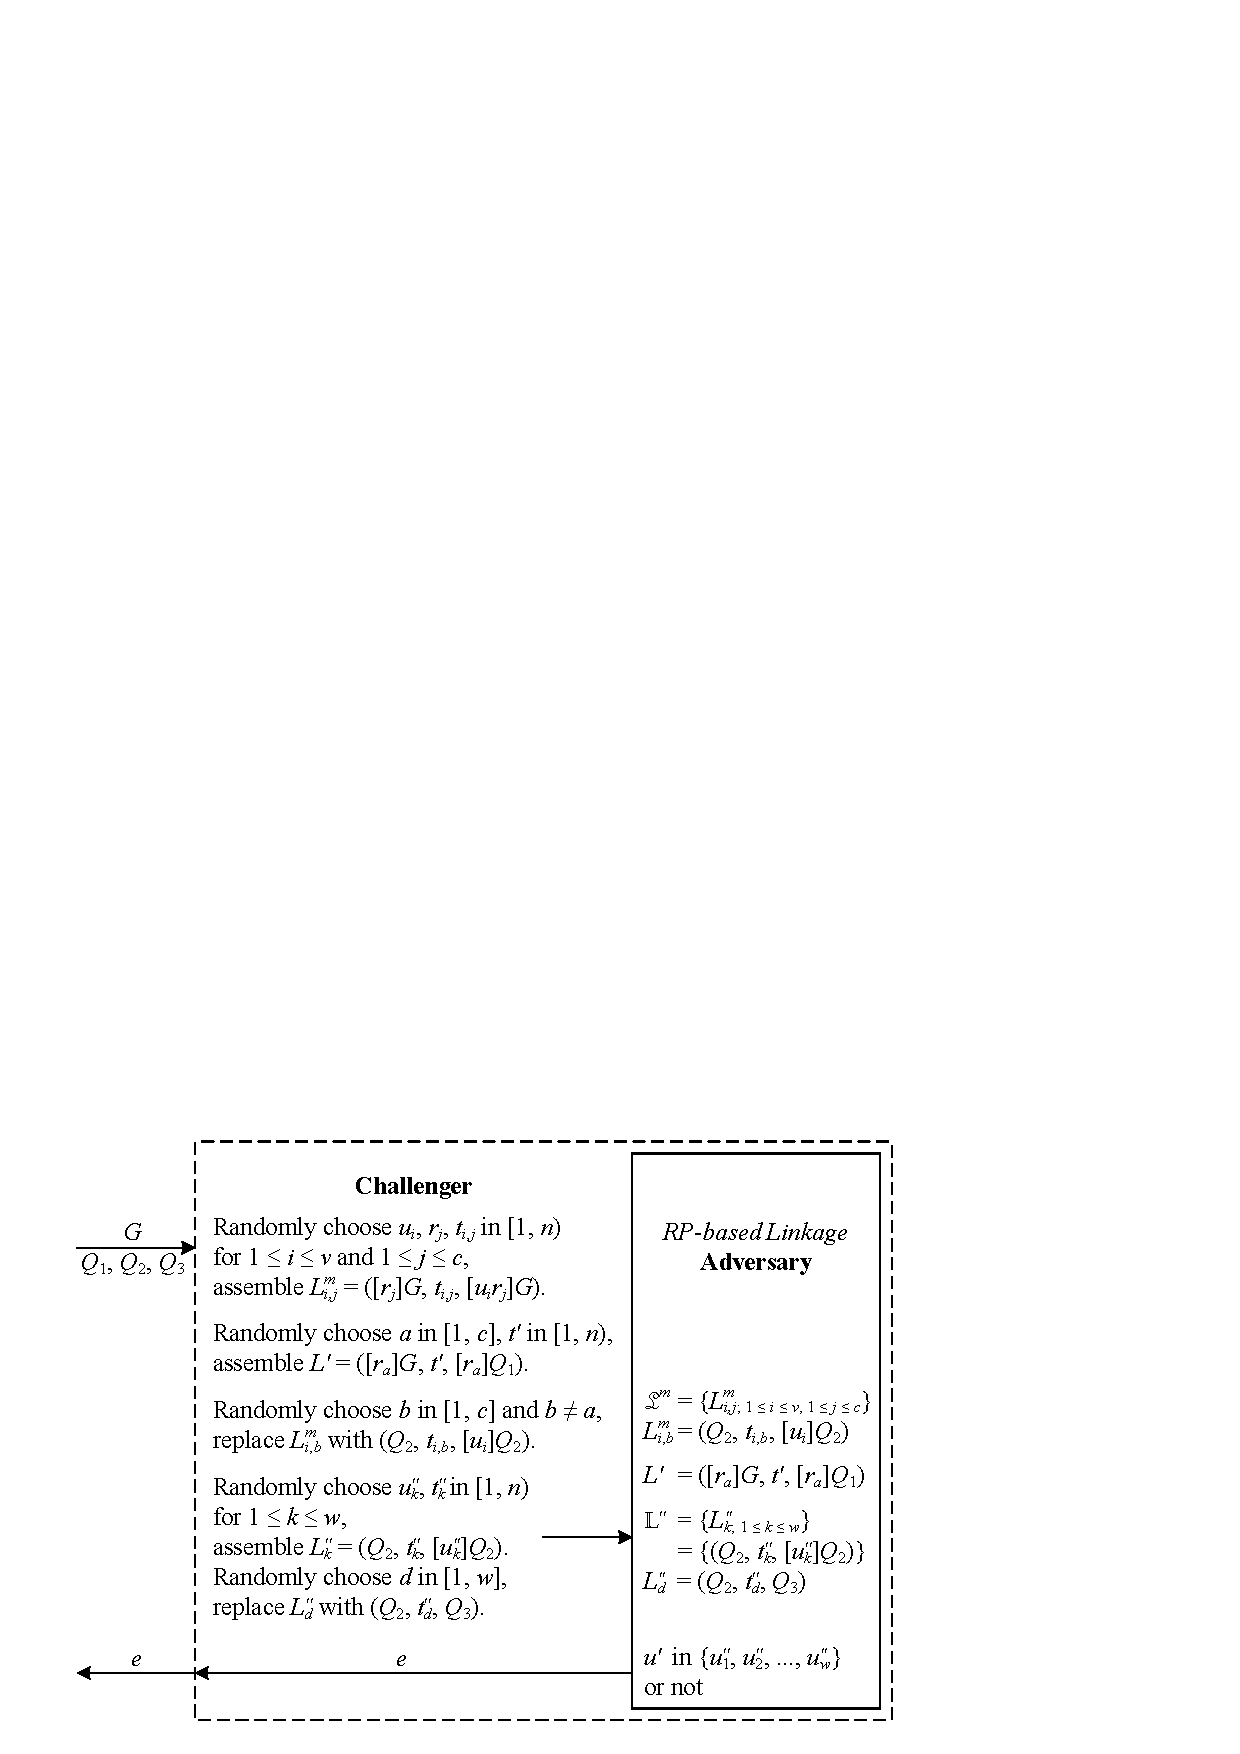
\includegraphics[width=1.0\linewidth]{fig/rp-linkage-game.pdf}
    \caption{The PPT algorithm $\mathcal{D}^*_r$ constructed based on the RP-based linkage game to solve the ECDDH problem.}
    \label{fig:dalgorithm}
  \end{figure}


  The algorithm $\mathcal{D}^*_r$ works as below. (1) Upon receiving an input $(G, Q_1=[x]G, Q_2=[y]G, Q_3=[z]G)$, %of $\mathcal{D}^*_r$
  the challenger
  chooses random numbers in $\mathbb{Z}_n$ to construct $\{u_i\}$, $\{r_j\}$, and $\{t_{i, j}\}$ for $1 \le i \le v$ and $1 \le j \le c$, with which it assembles $L^m_{i, j}=([r_j]G, t_{i,j}, [u_ir_j]G)$.
  In this process, it ensures $[r_{j}]G \neq Q_2$ so that $r_j \neq y$.  % 这个应该反过来讲;因为y是离散对数。
  (2) It randomly chooses $a \in [1, c]$ and $t' \in \mathbb{Z}_n$, to assemble $L' = ([r_{a}]G, t', [r_{a}]Q_1) = ([r_{a}]G, t', [xr_{a}]G)$.
  (3)
  % Here, $L'$ represents the knowledge of the login visiting $RP_{j'}$ by a user with $ID_U = x$.
  Next, the challenger randomly chooses $b \in [1, c]$ and $b \neq a$, and replaces $ID_{RP_b}$ with $Q_2 = [y]G$.
  Hence, for $1 \le i \le v$, the challenger replaces $L^m_{i, b}=([r_b]G, t_{i,b}, [u_ir_b]G)$ with $(Q_2, t_{i,b}, [u_i]Q_2) = ([y]G, t_{i,b}, [u_iy]G)$, and then constructs $\mathfrak{L}^m$.
  (4) the challenger chooses random numbers in $\mathbb{Z}_n$ to construct $\{u''_k\}$ and $\{t''_k\}$ for $1 \leq k \leq w$,
  with which it assembles $\mathbb{L}'' = \{L''_{k; 1\leq k \leq w}\} = \{(Q_2, t''_k, [u''_k]Q_2)\} = \{([y]G, t''_k, [u''_ky]G)\}$.
  In this process, it ensures that $[u''_k]G \neq Q_1$ (i.e., $u''_k \neq x$) and $u''_k \neq u_i$,
  for $1 \le i \le v$ and $1 \le k \le w$.
  Finally, it randomly chooses $d \in [1, w]$ and replaces $L''_{d}$ with $(Q_2, t''_d, Q_3) = ([y]G, t''_d, [z]G)$.
  Thus, $\mathbb{L}'' = \{L''_{k;1\leq k \leq w}\}$ represents the logins initiated by $w$ honest users, i.e., $\mathbf{u}_w=\{u''_1, u''_2, \cdots, u''_{d-1}, z/y, u''_{d+1}, \cdots, u''_w\}$.
  (5) When the adversary of $\mathcal{G}_r$ receives $\mathfrak{L}^m$, $L'$, and $\mathbb{L}''$ from the challenger, it returns $s$ as the output of $\mathcal{D}^*_r$.

  According to the above construction, % of $\mathfrak{L}$, $L'$ and $\mathbb{L}''$,
  $x$ is embedded as $ID_{U'}$ in the login $L'$ visiting the RP with $ID_{RP_{a}} = [r_{a}]G$,
  and $z/y$ is embedded as $ID_{U''_d}$ in $\mathbb{L}''$ visiting the RP with $ID_{RP_{b}}=[y]G$,
  together with $\{u''_1, \cdots, u''_{d-1}, u''_{d+1}, \cdots, u''_w\}$.
  Meanwhile, $[r_{a}]G$ and $[y]G$ are two malicious RPs' identities in $\mathfrak{L}^m$.
  Because $x \neq u''_{k; 1\leq k \leq w, k \neq d}$ and then $x$ is not in $\{u''_1, \cdots, u''_{d-1}, u''_{d+1}, \cdots, u''_w\}$, the adversary outputs $s=1$ and succeeds in the game \emph{only if} $x = z/y$.
  % 这里不是if and only if. "if, 就变成了the adversary必胜了;并不是,而是“有显著的概率”"
  % 当“the adversary outputs s=1 且 succeeds in the game”,=> "x = z/y"
  % 但是,"x = z/y"  => 不能推导得到“the adversary outputs s=1 且 succeeds in the game”。因为adversary有时候fail、不总是succeed
  Therefore, using $\mathcal{D}^*_r$ to solve the ECDDH problem, we have an advantage $\mathbf{Adv}^*=|{\rm Pr}^*_1 - {\rm Pr}^*_2|$, where
  \begin{align*}
  &{\rm Pr}^*_1 =  {\rm Pr}(\mathcal{D}^*_r(G, [x]G, [y]G, [xy]G)=1) \\
  =&{\rm Pr}(\mathcal{G}_r(\mathfrak{L}^m, L', \mathbb{L}'')=1 \; | \; u' \in \mathbf{u}_w) = {\rm Pr}_1 \\
  &{\rm Pr}^*_2= {\rm Pr}(\mathcal{D}^*_r(G, [x]G, [y]G, [z]G)=1) \\
  =&{\rm Pr}(\mathcal{G}_r(\mathfrak{L}^m, L', \mathbb{L}'')=1 \; | \; u' \in \mathbb{Z}_n) = {\rm Pr}_2 \\
  &\mathbf{Adv}^*=|{\rm Pr}^*_1-{\rm Pr}^*_2|=|{\rm Pr}_1-{\rm Pr}_2|={\mathbf{Adv}}
  \end{align*}

  If in $\mathcal{G}_r$ the adversary has a non-negligible advantage, then $\mathbf{Adv}^*={\mathbf{Adv}}$ is also non-negligible regardless of the security parameter $\lambda$. This violates the ECDDH assumption. Therefore, the adversary has no advantage in $\mathcal{G}_r$ and cannot decide whether $L'$ is initiated by some user with an identity in $\mathbf{u}_w$ or by a user in the universal user set.
  Moreover, because $RP_b$ is any malicious RP, this proof can be easily extended from $RP_b$ to more colluding malicious RPs.
  \end{proof}

  With Theorem~\ref{rp-privacy-proof}, %we can have that Lemma~\ref{lemma:statically-equivalent} still holds true for the much more complicated model we state above. 
  %Therefore, we can do the similar analysis to prove that $\mathcal{U\!W\!S}^{priv}$ is still RP-private even if we add more RPs, honest users and malicious users into the system.
  we can have that even if colluding RPs and users share 
  $PID_U$s and other information observed in all the logins, 
  the attackers still cannot link any login from an honest user 
  to any other logins from any other honest users to these RPs. 
  Next we want to prove that our web systems $\mathcal{U\!W\!S}^{priv}$ 
  with colluding RPs and users is indistinguishable. 

  Here, we make our proof by contradiction.
  Assuming that the attacker cannot link any login but can 
  distinguish in our web systems for privacy analysis, 
  the attacker should be able to tell the difference between 
  $\mathcal{U\!W\!S}^{priv}_1$ and $\mathcal{U\!W\!S}^{priv}_2$.
  However, the only difference between two web systems is that 
  the same honest user login in the same RP in one system but 
  different users in the other, so the attacker can actually 
  link the login by the distinguishability. Therefore, there is 
  a contradication to the assumption, where we assumed that the 
  attacker cannot link any login. This shows $\mathcal{U\!W\!S}^{priv}$ 
  with colluding RPs and users is indistinguishable.

  This proves Theorem~\ref{theorem:rp-privacy}.\QED
  
\end{document}
